% Motivation
    %% Coating Thermal Noise
	%%% Brownian Thermal Noise
	    %%%% Internal Friction in Materials and Loss Angle
    	    %%%% Coating Brownian Thermal Noise
    	    %%%% Silica Ti-Tantala coating parameters
    	    %%%% GaAs/AlGaAs coating parameters
    %% Anisotropic Media
	%%% The Dielectric Tensor
    	%%% Indicatrix
    	%%% Linear Electro-optic Effect (Pockel's Effect)
    	%%% Electro-optic coefficients r_ij for zincblende crystals
    	%%% New Principal (electro-optic) dielectric constants for zincblende structures
    	%%% The photoelastic effect
    	%%% The generalized indicatrix
    %% EO modulation
    %% Optical anisotropy of an HR GaAs / AlGaAs stack
    %% Miller indices for HR GaAs / AlGaAs coatings
        %%% Electro-optic coupling to the reflected phase of a HR mirror coating
    %% Numerical estimate
    %% Measured birefringence from HR \texorpdfstring{$\gaas$}{gaas}/\texorpdfstring{$\algaas$}{algaas} mirrors
    %% Initial projected DARM coupling

% Electro-optic measurement apparatus
    %% PDH servo
    %% Servo Parameters
	%%% Sensing S(f)
    	%%% Actuation A(f)
    	%%% Low Frequency Servo (Thermal Loop)
    	%%% OLG(f) 
    %% Longitudinal Pockels Cell mirror mount assembly
	%%% Modeling
    	%%% Voltage drive electronics
    %% Servo Overview
    %% Calibration

% Results
    %% Mounting Strategies
	%%% Assembly 1
    	%%% Assembly 2
    	%%% Assembly 3 (MACOR mount)
    	%%% Acousto-optical coupling

% Conclusion
\section{Motivation}
Contributions of categorized noises for gravitational wave detectors are organized in a ``noise budget" (i.e. \autoref{fig:aplusasharp} and \autoref{fig:high_freqnoise}): comprised of a collection of technical (noise imposed by the practical operation of the detector) and fundamental (inherent physical limitations of the DRFPMI design) noise that limit gravitational wave detection. Understanding how much differential phase noise is imparted on the interferometer carrier light passing through and reflecting from core optics is crucial.

\subsection{Coating Thermal Noise}
%% Contributions of categorized noises for gravitational wave detectors the ''noise budget" ((LHO and LLO O3?) or just GWINC?)}
One source of noise in high precision optical experiments operating at room temperature (and higher due to high power resonant beams), can be realized through Brownian thermal noise and the Fluctutaion dissapation theorem. 

\subsubsection*{Brownian Noise}
In 1827 the Scottish botanist Robert Brown observed a constant motion of pollen particulates on the surface of water; witnessing randomized collisions of the water molecules holding a kinetic energy proportional to the temperature ($k_BT$) \cite{brown:1828}. It is because of these documented observations we name the phenomena Brownian motion. And although the observations were on motion of particulates in liquids and gases, solids also exhibit similar fluctuations through their modes of dissipation. 

\subsubsection*{Fluctuation Dissipation Theorem}
Any movement / fluctuations at finite temperatures of the core optic components is especially important for GWDs and becomes more clear when reviewing the fluctuation dissipation theorem (FDT). Derived by H.B. Callen and T.A. Welton, the theorem states that for a randomly fluctuating linear force ($F_x^2(f)$) \cite{callen:1951}:

%% Further insight into Brownian motion was explored by Einstein where he was able to relate the mean-square displacement of a particle of radius $r_\mathrm{sph}$ on a fluid with viscosity $\eta$.
 %%\begin{equation}
 %%\overline{x^2} = k_B T  \frac{1}{3 \pi \eta  r_\mathrm{sph}}
 %%\end{equation}
 %%This relation has important implications about how the random motion or fluctuations of a particulate (the pollen) is influenced (dissipated) by the viscosity of the surrounding medium (water).

\begin{equation}
F_x^2(f) = 4 k_B T\; \Re[Z]
\end{equation}

\noindent Where $\Re[Z]$ is the real part of the impedance of the system. This impedance directly relates to equations of motion:

 \begin{equation}
 Z = \frac{F}{\dot{x}}
 \end{equation}

 \noindent Another useful form is the power spectrum of the fluctuating motion:

\begin{equation}\label{eq:fdtpsd}
x^2 (f)  = \frac{4k_B T}{(2 \pi f)^2}\; \Re[Y]
\end{equation}

\noindent Where $Y$ is the inverse impedance or admittance. The root mean square (RMS) displacement ($x^2(f)$) as informed by the FDT facilitates modelling and budgeting notable Brownian noise sources that fundamentally limit LIGO (i.e. by choice of materials used for highly reflective mirror coatings). Though adequate modelling of internal force couplings for the aforementioned components provides a more complete picture.

\subsubsection*{Internal friction in materials and loss angle}
Zener provides a model of the internal friction of materials incorporating anelasticity into the equations of motion \cite{zener:1948}:
\begin{equation}
F = k(1+i\phi)x + m\ddot{x}
\end{equation}

\noindent Where $m$ is mass attached to a spring with a spring constant $k(1+ i\phi)$ incorporating the degree of anelasticity $\phi$. From equations 3.5 and 3.3 we perform a Laplace transform and acquire the following form of admittance:
\begin{equation}
Y(s) = \frac{\dot{x}(s)}{F(s)} = \frac{-s}{k(1+i\phi) + ms^2}
\end{equation}

\noindent Or more transparently the Fourier representation since we assume a linear time invariant system:

\begin{equation}\label{eq:admitint}
Y(\omega) = \frac{\dot{x}(\omega)}{F(\omega)} = \frac{-i\omega}{k(1+i\phi) - m\omega^2} = \frac{k \omega \phi - i \omega (k - m \omega^2)}{(k-m\omega^2)^2 +k^2 \phi^2}
\end{equation}

\noindent Plugging equation \autoref{eq:admitint} back into \autoref{eq:fdtpsd}:

\begin{equation}
x^2 (f)  = \frac{2k_B T}{\pi}\frac{k\phi}{(k-4\pi^2 m f^2)^2 + k^2 \phi^2}
\end{equation}

Computing the admittance from a Gaussian beam impinging upon a HR mirror can require expansion of all individual mechanical degrees of freedom of the test mass system across a relevant frequency range, and with such an approach convergence is not guaranteed. Saulson and Gonzalez provide an alternative method to computing the admittance coined the ``direct approach" by Levin when computing the noise from a Gaussian beam on a LIGO HR test mass. The admittance can be acquired through:

\begin{equation}\label{eq:admitdirec}
\Re[Y] = \frac{W_\mathrm{diss}}{F_o^2}
\end{equation}

\noindent $W_\mathrm{diss}$ is the dissipated power from the system due to an oscillating force $F_o$. This form of the admittance reveals an important result of the fluctuation dissapation theorem where an undriven system with a dissapative actor, imparts motion to the degrees of freedom via a driving force by virtue of that same actor at finite temperatures. This direct approach also allows the surface pressure applied by the Gaussian beam to interrogate which mechanical modes of the test mass impose a significant energy when \autoref{eq:admitdirec} is plugged into \autoref{eq:fdtpsd}. In the case of the gaussian beam / uncoated test mass studied by Levin \cite{levin:1998}:

\begin{equation}
S_x(f) = \frac{4 k_B T}{f} \frac{1-\sigma^2}{\pi^3 E_o r_o} I\phi \bigg[1- O\bigg( \frac{r_o}{R} \bigg)\bigg]
\end{equation}

%this requires that the driving force used in a lab mimics that of a force from a centered Gaussian beam.

%%Refer to Levin appendix for more on how elasticity parameters are introduced?
\noindent Where $\sigma$ and $E_o$ are the Poisson ratio and Young's modulus respectively, and $O(\frac{r_o}{R})$ is a correction term as a function of the small beam radius ($r_o$) relative to the mirror radius ($R$).

\subsubsection*{Thermal noise of HR mirror coatings}
Further investigations into the beam/optic system utilizing this approach and elasticity theory led to a deeper understanding about Brownian thermal noise contributions from LIGO test masses (substrate, suspensions, HR coating). Levin mentions, with further detail from Harry, that the noise contributed by a lossy mirror coating is proven to be to be the most significant contributor of brownian thermal noise ~\cite{harry:2006}. Hong provides a power spectral density \cite{hong:2013}:

\begin{equation}
S_j^X = \frac{4k_B T \lambda \phi_x^j(1- \sigma_j - 2 \sigma_j^2)}{3 \pi^2 f Y_j (1-\sigma_j)^2 \omega_o^2}
\end{equation}

\noindent Where X represents bulk and shear with j = odd (material 1) and j = even (material 2) alternating layers representing high and low index materials j = odd (material 1) j = even (material 2) for an HR coating.

\begin{figure}[H]
    \begin{center}
    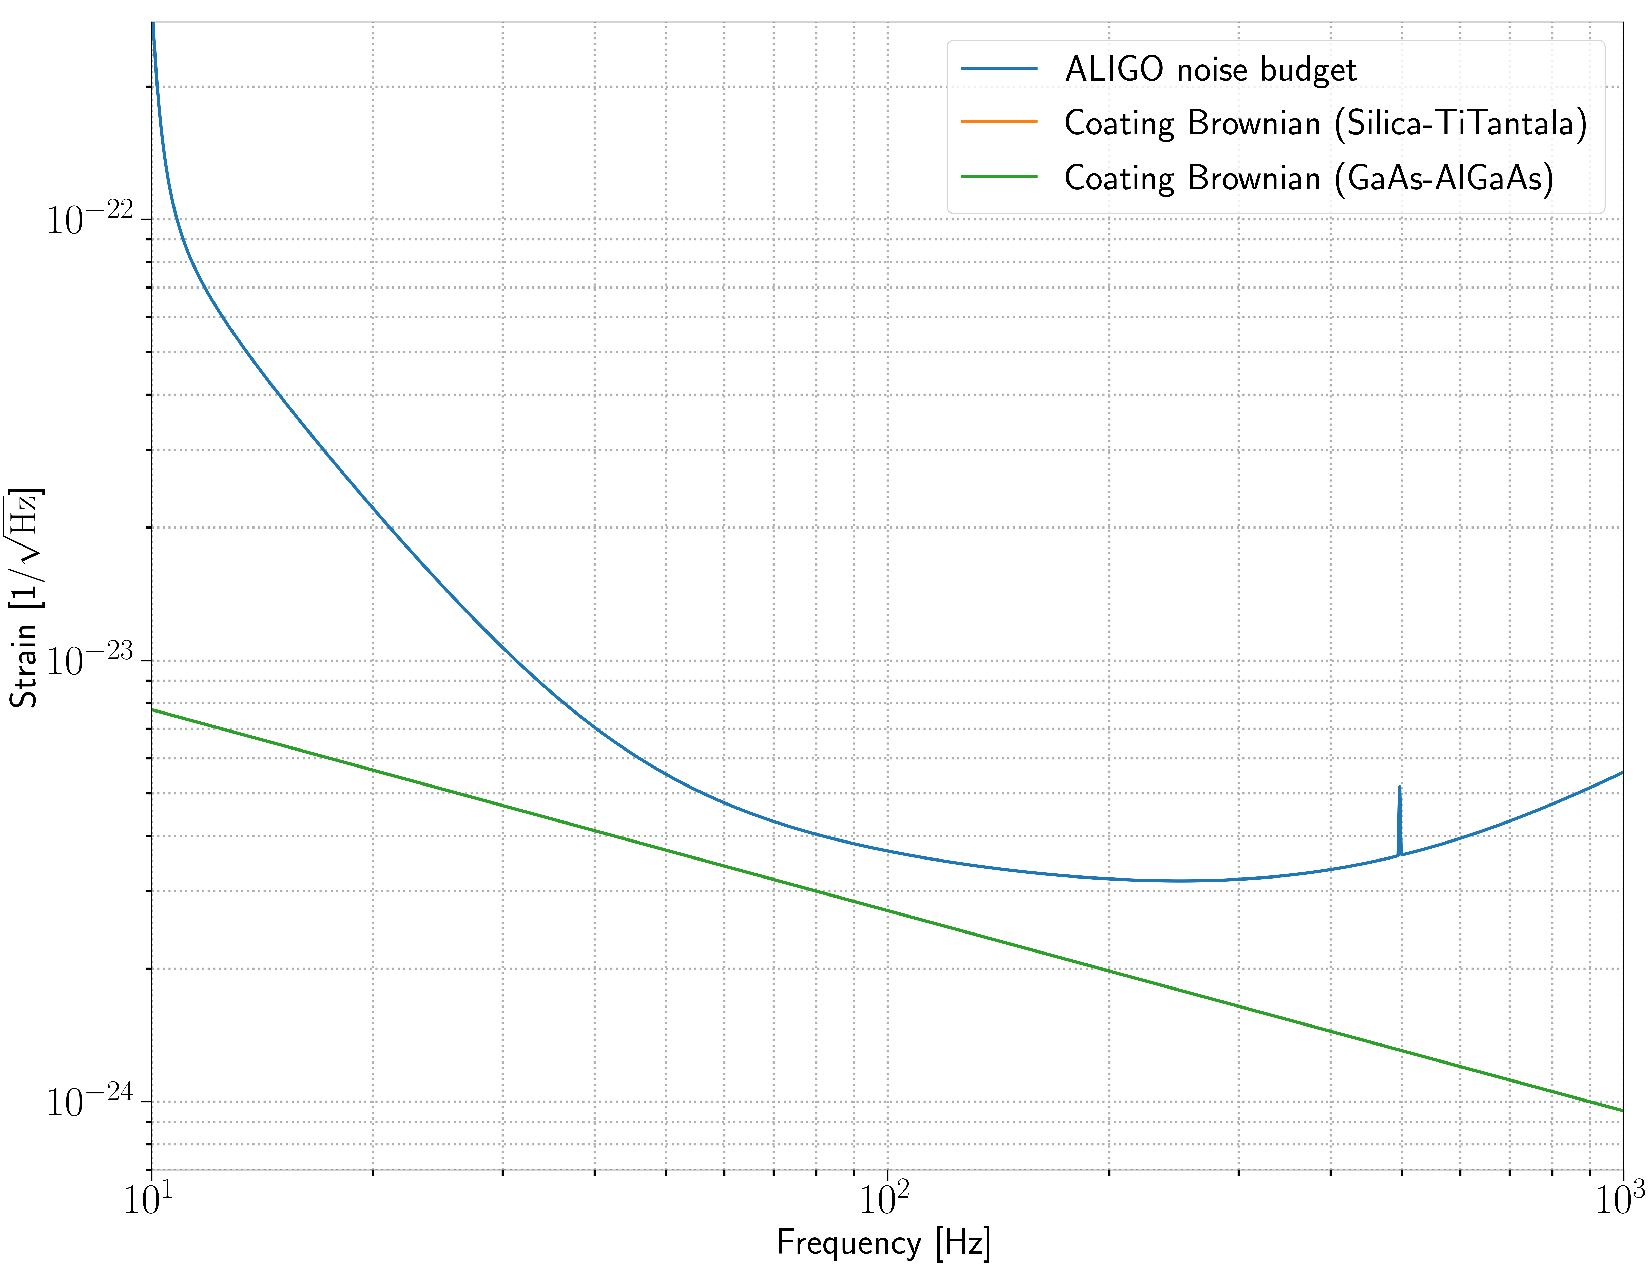
\includegraphics[width=.9\textwidth]{ALGAAS/aligo_nb_plus_cbn.pdf}
    \end{center}
    \caption{\textcolor{red}{ALIGO noise budget placeholder} for silica-tantala, and gaas-algaas brownian noise comparison}
\label{fig:aligotncomp}
\end{figure}

%% Coating params table?
%\paragraph{$\siotao$ coating parameters} 
%Currently the LIGO interferometers deposit $\lambda$/4 stacks of silica and titania doped tantala on fused silica test mass substrates. Effective loss angle measurements \cite{harry:2006}
%
%\textbf{Current $\siotao$ elasticity params, power spectra, and strain spectral density (order of magnitude estimate)}
%
%\paragraph{$\gaas$/$\algaas$ coating parameters}
%%%Specific coating parameters for most promising $\algaas$ candidates? Chat with Steve. Or just mention parameters that are listed in Cole 2013
%\cite{cole:2013}
%
%%% Insert computed curves of the most precise and recent (effective) loss angle measurements (Nick Demos measurements?). More instructive to plot strain spectral density or displacement power spectra
%
%\noindent Currently thermal noise from the $\siotao$ optical coatings is the largest contributor of Brownian noise in LIGO compared to estimated substrate and suspension thermal noise \cite{harry:2006}. As of the end of O3, Brownian thermal noise is estimated to be ? orders of magnitude below the current sensitivity and it will prove to be the limiting source of noise as that sensitivity is increased with various other upgrades mitigating fundamental and technical noise. 
%%% Already mentioned in intro prior to this thermal noise section. Need to re-iterate in more detail?



As aLIGO approaches designed sensitivity, the thermal noise limit set by $\siotao$ HR coatings becomes an immediate limit to further improvements. Though there are proposals for the usage of alternative mirror coating solutions to push down this thermal noise limit for increased detector sensitivity \cite{harry:aigwd2019}. $\gaas$/$\algaas$ is a crystalline coating candidate showing promise for next generation detectors with reduced coating Brownian noise by a factor of 10, cooresponding to a potential strain reduction by a factor of 5 ~\cite{cole:2013} when compared to the current aLIGO coating thermal noise limit. 

\subsection{Coating Electro-optic Noise}
Applying crystalline HR mirror coatings to the core optics indiscriminately may introduce notable side effects; one being linear electro-optic noise of $\gaas$/$\algaas$ (dn/dE), also known as the Pockels effect ~\cite{abernathy:poster}. Although estimated to be nearly two orders of magnitude below the A$^\sharp$ strain noise floor ($\approx 10^{-26}$), direct measurement is still merited and adequately motivates a thorough study of electro-optical properties of $\gaas$/$\algaas$ coatings. The rest of this chapter discusses such a study by detailing: 1) birefringence in zincblende materials, 2) a preliminary estimation of differential phase noise of light reflected from a $\gaas$/$\algaas$ coating stack caused by electric field noise are computed while considering potential impacts to the current generation gravitational wave detectors, and 3) a short experimental optical cavity designed to interrogate an estimate of dn/dE from a calibrated differential length PDH locked signal with a normal electric field driven across a HR $\gaas$/$\algaas$ coating ``witness" sample.

\section{Birefringence in zincblende materials}
\subsection{The Indicatrix}\label{sec:indicatrix}
The two index solutions for a uniaxial crystal given a general plane wave with unit wave vector $\vec{k}$ can be found via a conveniant geometrical construction known as the ``index ellipsoid". 

\begin{figure}[ht!]
\begin{center}
\includegraphics[width=.85\textwidth]{figs/ALGAAS/indicatrix_alph.pdf}
\end{center}
\caption{A surface of uniform energy density ($U_E$) forming an ellipsoid in D-space for a generalized uniaxial crystal with general wavefront propogation indicated by a plane normal $\hat{k'}$ where the major and minor axes of the ellipse cross section indicate slow and fast axes $n_\beta$ and $n_\alpha$ respectively.}
\label{fig:genindtrx}
\end{figure}

The construction begins when considering a constant electric energy density ($U_e$) surface in the $\vec{D}$ space; which forms an ellipsoid: 

\begin{equation}\label{eq:lagr1}
\frac{D_x}{\varepsilon_x} + \frac{D_y}{\varepsilon_y} + \frac{D_z}{\varepsilon_z} = 2 U_e \varepsilon_o
\end{equation}
With redefined coordinates $(\vec{D}/\sqrt{2 U_e \varepsilon_o}) \rightarrow \vec{r}$ and setting $\varepsilon_i = n^2_i$:
\begin{equation}
\frac{x^2}{n_x^2} + \frac{y^2}{n_y^2} + \frac{z^2}{n_z^2} = 1
\end{equation}

This equation for the ellipsoid is known as the indicatrix. Given the co-planar solution demonstrated in \autoref{appendix:Diel_tensor}, we can impose the normal of the plane $\vec{r} \cdot \vec{s} = 0$:

\begin{equation}\label{eq:lagr2}
\vec{r} \cdot \vec{s} = x s_x + y s_y + z s_z = 0
\end{equation}
\autoref{eq:lagr1} and \autoref{eq:lagr2} both contribute constraints to the method of finding extrema using Lagrange multipliers for the function:
\begin{equation}
r^2 = x^2 + y^2 + z^2
\end{equation}
The Lagrangian ($\mathcal{L}$) with the introduced multiplers ($\lambda_1$, $\lambda_2$) then becomes:
\begin{equation}
\mathcal{L}(\vec{r},\vec{s},\lambda_1, \lambda_2) =
x^2 + y^2 + z^2 + \lambda_1 (xs_x + ys_y + zs_z) + \lambda_2 \bigg( \frac{x^2}{\varepsilon_x} + \frac{y^2}{\varepsilon_y} + \frac{z^2}{\varepsilon_z} - 1 \bigg)
\end{equation}
With the generated system of equations from the Lagrange multipler method ($\partial F_i/ \partial x_i = 0$, and $\partial F_j/ \partial \lambda_j$) where index $i =x,y,z$ and $j = 1,2$ we obtain a system of 3 equations:
\begin{equation}
i \bigg(1-\frac{r^2}{\varepsilon_{i}} \bigg) + s_{i} \bigg(\frac{x s_x}{\varepsilon_x} + \frac{y s_y}{\varepsilon_y} + \frac{z s_z}{\varepsilon_z} \bigg) = 0
\end{equation}
The result is verified when substituting $r \rightarrow \frac{\vec{D}}{\sqrt{\vec{E} \cdot \vec{D} \varepsilon_o}}$ back which recovers \autoref{eq:modelec}.
\\
\subsection{\texorpdfstring{$\gaas$}{gaas} and \texorpdfstring{$\algaas$}{algaas} crystal classification}
$\gaas$ as well as $\algaasgen$ are both within the $F\bar{4}3m$ space group. Crystals of this space group are commonly known as zincblende crystals; a common crystal configuration named after zinc sulfide (ZnS). Also categorized as a cubic crystal, their crystallographic structure displays linear optical isotropy when stress free and no DC and/or slowly varying electric fields are present~\cite{boyd:2008}. 

\begin{figure}[!ht]
\begin{center}
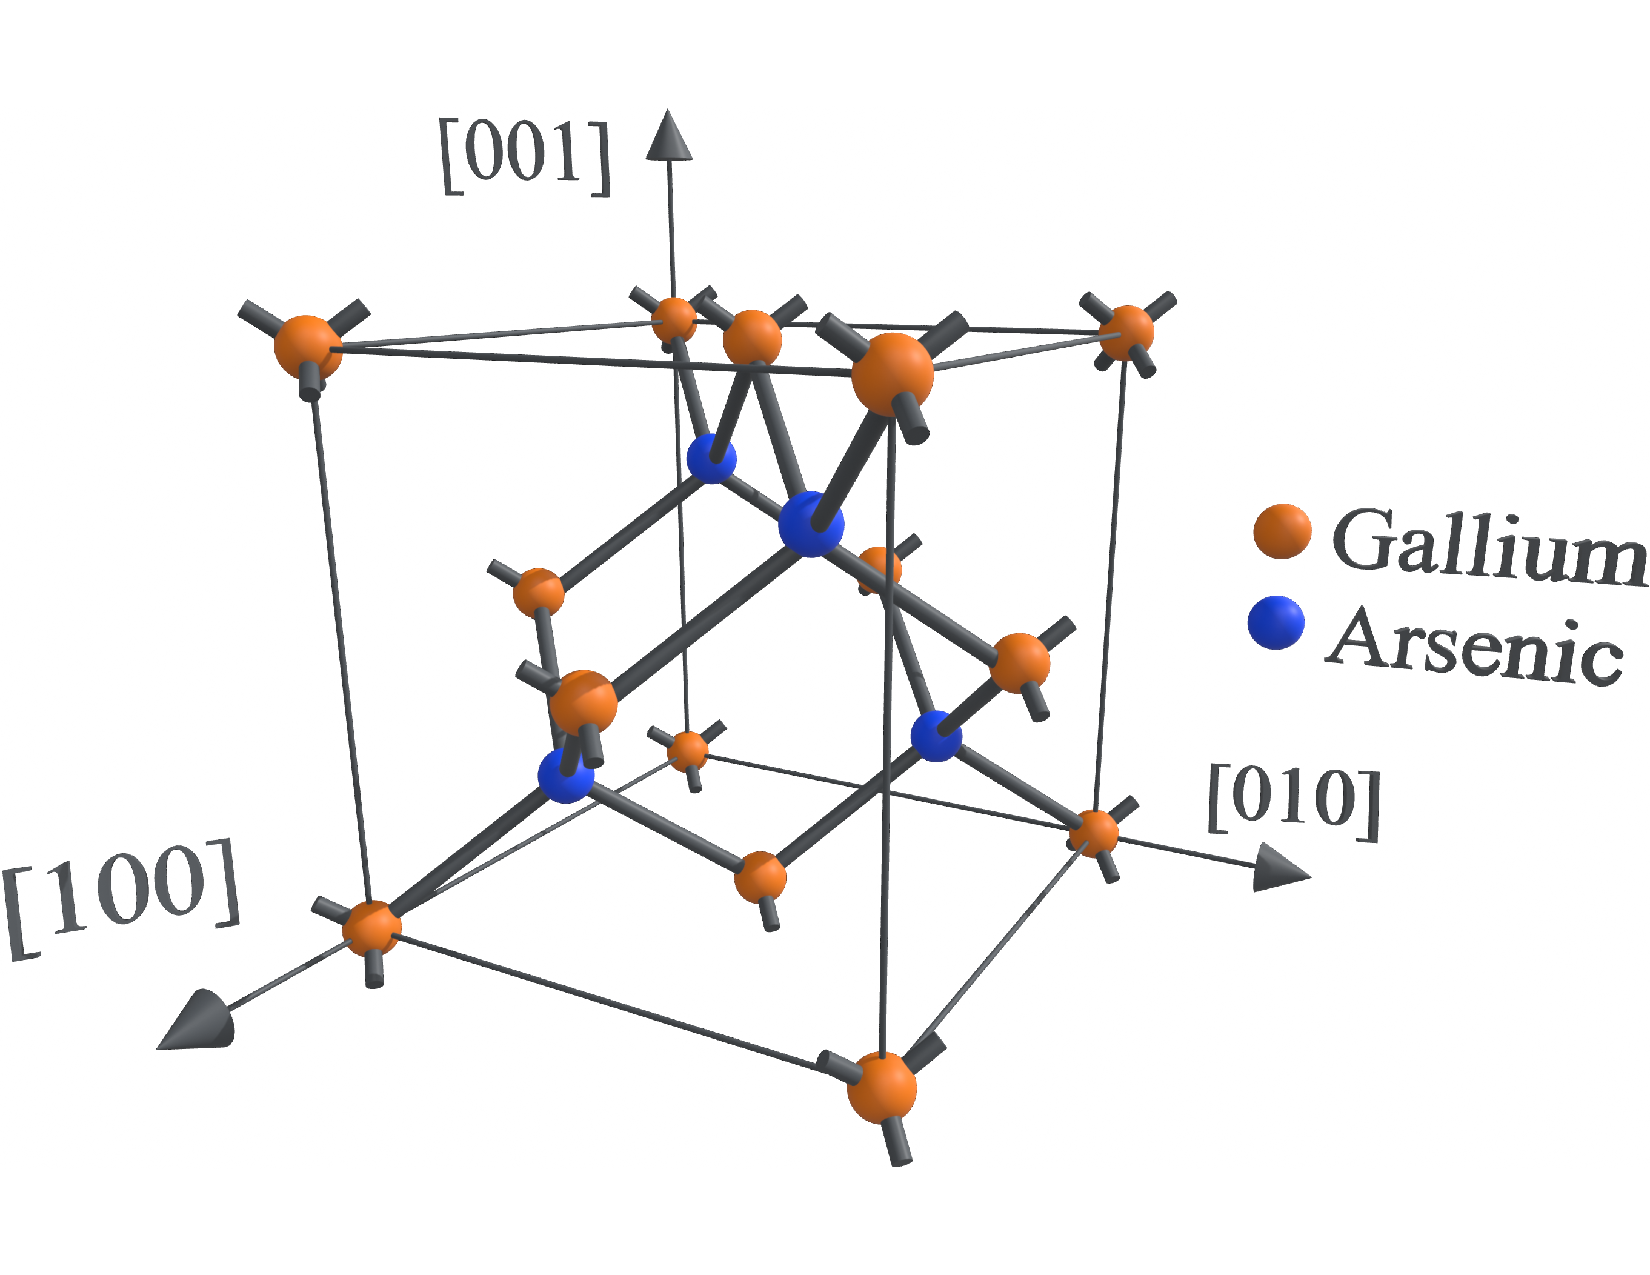
\includegraphics[width=.5\textwidth]{figs/ALGAAS/gaas_unit_cell_mi.pdf}
\caption{The unit cell of gallium arsenide (GaAs) with associated miller indices as coordinate axes}
\end{center}
\label{fig:gaasuc}
\end{figure}

Zincblende structures, like the crystalline materials in question can exhibit birefringent properties when under influence of mechanical stresses and static / low-frequency electric fields ($E_\mathrm{STLF}$); characterized by photoelastic and electro-optic effects respectively. For realistic mirror coatings, heteroepitaxial bonding between $\gaas$/$\algaas$ layers (potentially from a noticiable difference in lattice cell constant) may produce an intrinsic strain within the HR stack and can lead to the existence of a static non-negligible birefringence throughout the coating layers \cite{cole:2016, adachi:1985}.

\subsection{Linear electro-optic effect (Pockel's effect)}
For non-centrosymmetric crystalline media there exists a non-zero rank 2, $6 \times 3$ tensor ($r_{ij}$) connecting low-frequency \footnote{``low frequency'' meaning orders of magnitude smaller relative to an optical field} electric fields $\vec{E_{STLF}}(f) = [E_x(f), E_y(f), E_z(f)]$ directly to the \hyperref[sec:indicatrix]{indicatrix} ~\cite{yariv,nye}:
\begin{equation}
  \left[ {\begin{array}{c}
   \big( \frac{1}{\Delta n ^2 } \big)_1 \\
   \big( \frac{1}{\Delta n ^2 } \big)_2 \\
   \big( \frac{1}{\Delta n ^2 } \big)_3 \\
   \big( \frac{1}{\Delta n ^2 } \big)_4 \\
   \big( \frac{1}{\Delta n ^2 } \big)_5 \\
   \big( \frac{1}{\Delta n ^2 } \big)_6 \\
  \end{array} } \right]
  =
%
 \left[ {\begin{array}{ccc}
   r_{11} & r_{12} & r_{13}\\
   r_{21} & r_{22} & r_{23}\\
   r_{31} & r_{32} & r_{33}\\
   r_{41} & r_{42} & r_{43}\\
   r_{51} & r_{52} & r_{53}\\
   r_{61} & r_{62} & r_{63}\\
  \end{array}} \right]
 %
 \left[{\begin{array}{c}
   E_x (f)\\
   E_y (f)\\
   E_z (f)\\
 \end{array}} \right]
\end{equation}

\noindent The $i$ index runs over the terms in the indicatix equation:
\begin{equation}
\bigg(\frac{1}{\Delta n_x^2} \bigg) x^2\ + \bigg(\frac{1}{\Delta n_y^2} \bigg) y^2 + \bigg(\frac{1}{\Delta n_z^2} \bigg) z^2 + 2 \bigg(\frac{1}{\Delta n_{xz}} \bigg)xz + 2 \bigg(\frac{1}{\Delta n_{yz}} \bigg)yz + 2 \bigg(\frac{1}{\Delta n_{xy}} \bigg)xy = 1
\end{equation}

%%Detail on some prior knowledge of $f \leq f_\mathrm{max}$? (Pockels cell specs?)

\subsubsection{\texorpdfstring{$r_{ij}$}{rij} for zincblende crystals (\texorpdfstring{$r_{\bar{4}3m, ij}$}{r43})}

The form of the electro-optic tensor for zincblende crystals (including $\gaas$ and $\algaas$) reduces such that $r_{ij} = r_{41} = r_{52} = r_{62} \neq 0$ with all other terms being zero:

\begin{equation}
r_{\bar{4}3m,ij} =
 \left[ {\begin{array}{ccc}
  0 & 0 & 0\\
  0 & 0 & 0\\
  0 & 0 & 0\\
  r_{41} & 0 & 0\\
  0 & r_{52} & 0\\
  0 & 0 & r_{63}\\
 \end{array}} \right]
\end{equation}

\noindent Where $r_{41} = r_{52} = r_{63}$

\subsection{New principal (electro-optic) dielectric axis for zincblende structures}
In general the principle dielectric axes of the new ellipsoid do \textbf{not} coincide with the axes of the ellipsoid of the unperturbed crystal. The form of the index ellipsoid for a zincblende crystalline material accounting for the electro-optic tensor and some generalized DC electric field $\vec{E}$ expressed in terms of the crystallographic axes is given by:
\begin{equation}\label{eq:zindicatrix}
\bigg(\frac{1}{n_o^2} \bigg) x^2\ + \bigg(\frac{1}{n_o^2} \bigg) y^2 + \bigg(\frac{1}{n_o^2} \bigg) z^2  + 2r_{41} E_{x} yz + 2r_{41} E_{y} xz + 2r_{41}E_{z} xy= 1
\end{equation}

\noindent Where we have set $n_x = n_y = n_z = n_o$ for zincblende structures. Visualizing the above as a tensor:

\begin{equation}
\left[ {\begin{array}{ccc}
   \big( \frac{1}{n_o ^2} \big)& r_{41}E_{x} & r_{41} E_{y}\\
   r_{41}E_{x} & \big( \frac{1}{n_o ^2} \big) & r_{41} E_{z}\\
   r_{41} E_{y} & r_{41} E_{z} & \big( \frac{1}{n_o ^2} \big)\\
\end{array}} \right]
\end{equation}



\subsection{The photoelastic effect}

General stresses and strains of a material may also cause transformations to the indicatrix connected by the rank 4 elasto-optical tensor $p_{i j k l}$:

\begin{equation}
 \bigg( \frac{1}{\Delta n^2} \bigg)_{ij} = p_{ijkl} \epsilon_{kl}
\end{equation}

\noindent Where the strain ({\boldmath$\epsilon$}) relates to stress ({\boldmath$\sigma$}) using the generalized Hooke's law: 
%\begin{equation}\label{eq:indicgen_stress2strain}
%	\epsilon_{\alpha \beta} = r_{\gamma \alpha \beta}E_{\alpha} + s_{\alpha \beta \gamma \theta } \sigma_{\gamma \theta}
%\end{equation}
% elasto-optic ($p_{ij \alpha \beta}$) tensor to the stress tensor ($\epsilon_{\alpha \beta}$) via stress-strain / piezoelectric relations:
\begin{equation}\label{eq:genhookeslaw} 
 \begin{split}
	 \epsilon_{ij} = K_{ijkl} \sigma_{kl}
	 \\
	 \sigma_{ij} = C_{ijkl} \epsilon_{kl}
 \end{split}
\end{equation}
A connection is also formed between the elasto-optical tensor ({\boldmath$p$}) to the piezo-optical tensor ({\boldmath$\pi$}): 
\begin{equation}\label{eq:indicgenelastooptical}
 \begin{split}
	p_{ijkl} = \pi_{ijkl} C_{klrs}
	\\
	\pi_{ijrs} = p_{ijrs} K_{rskl}
 \end{split}
\end{equation}

\subsection{The generalized indicatrix}
Both forms of the induced birefringence (electro-optic and photo-elastic) can be incorportated into a condensed form \cite{nye}:

\begin{equation}\label{eq:indicgen}
	\bigg( \frac{1}{\Delta n^2} \bigg)_{ij} = r_{ijk}E_k + p_{ijkl} \epsilon_{kl}
\end{equation}


%%New principal dielectric axes for zincblende structures (zinblende photoelastic tensor, zincblende electro-optic tensor)

\subsection{EO Modulation (Application)}\label{sec:EOM}
Imparting phase modulations onto an optical carrier field is a common application of the electro-optic effect. Electro-optic modulators (EOMs) or Pockel cells are sold as a standard optical components usually composed of a monolithic crystalline material sandwiched between two capacitor plates connected to a single electrical input port (typically coaxial for RF) designed to take in a voltage input of frequency ($\Omega$) within a specified modulation amplitude and frequency bandwidth. When the field amplitude across the crystal is driven by a voltage controlled oscillation, the amplitudes of the electro-optic tensor vary linearly. 

\begin{figure}[H]
    \centering
    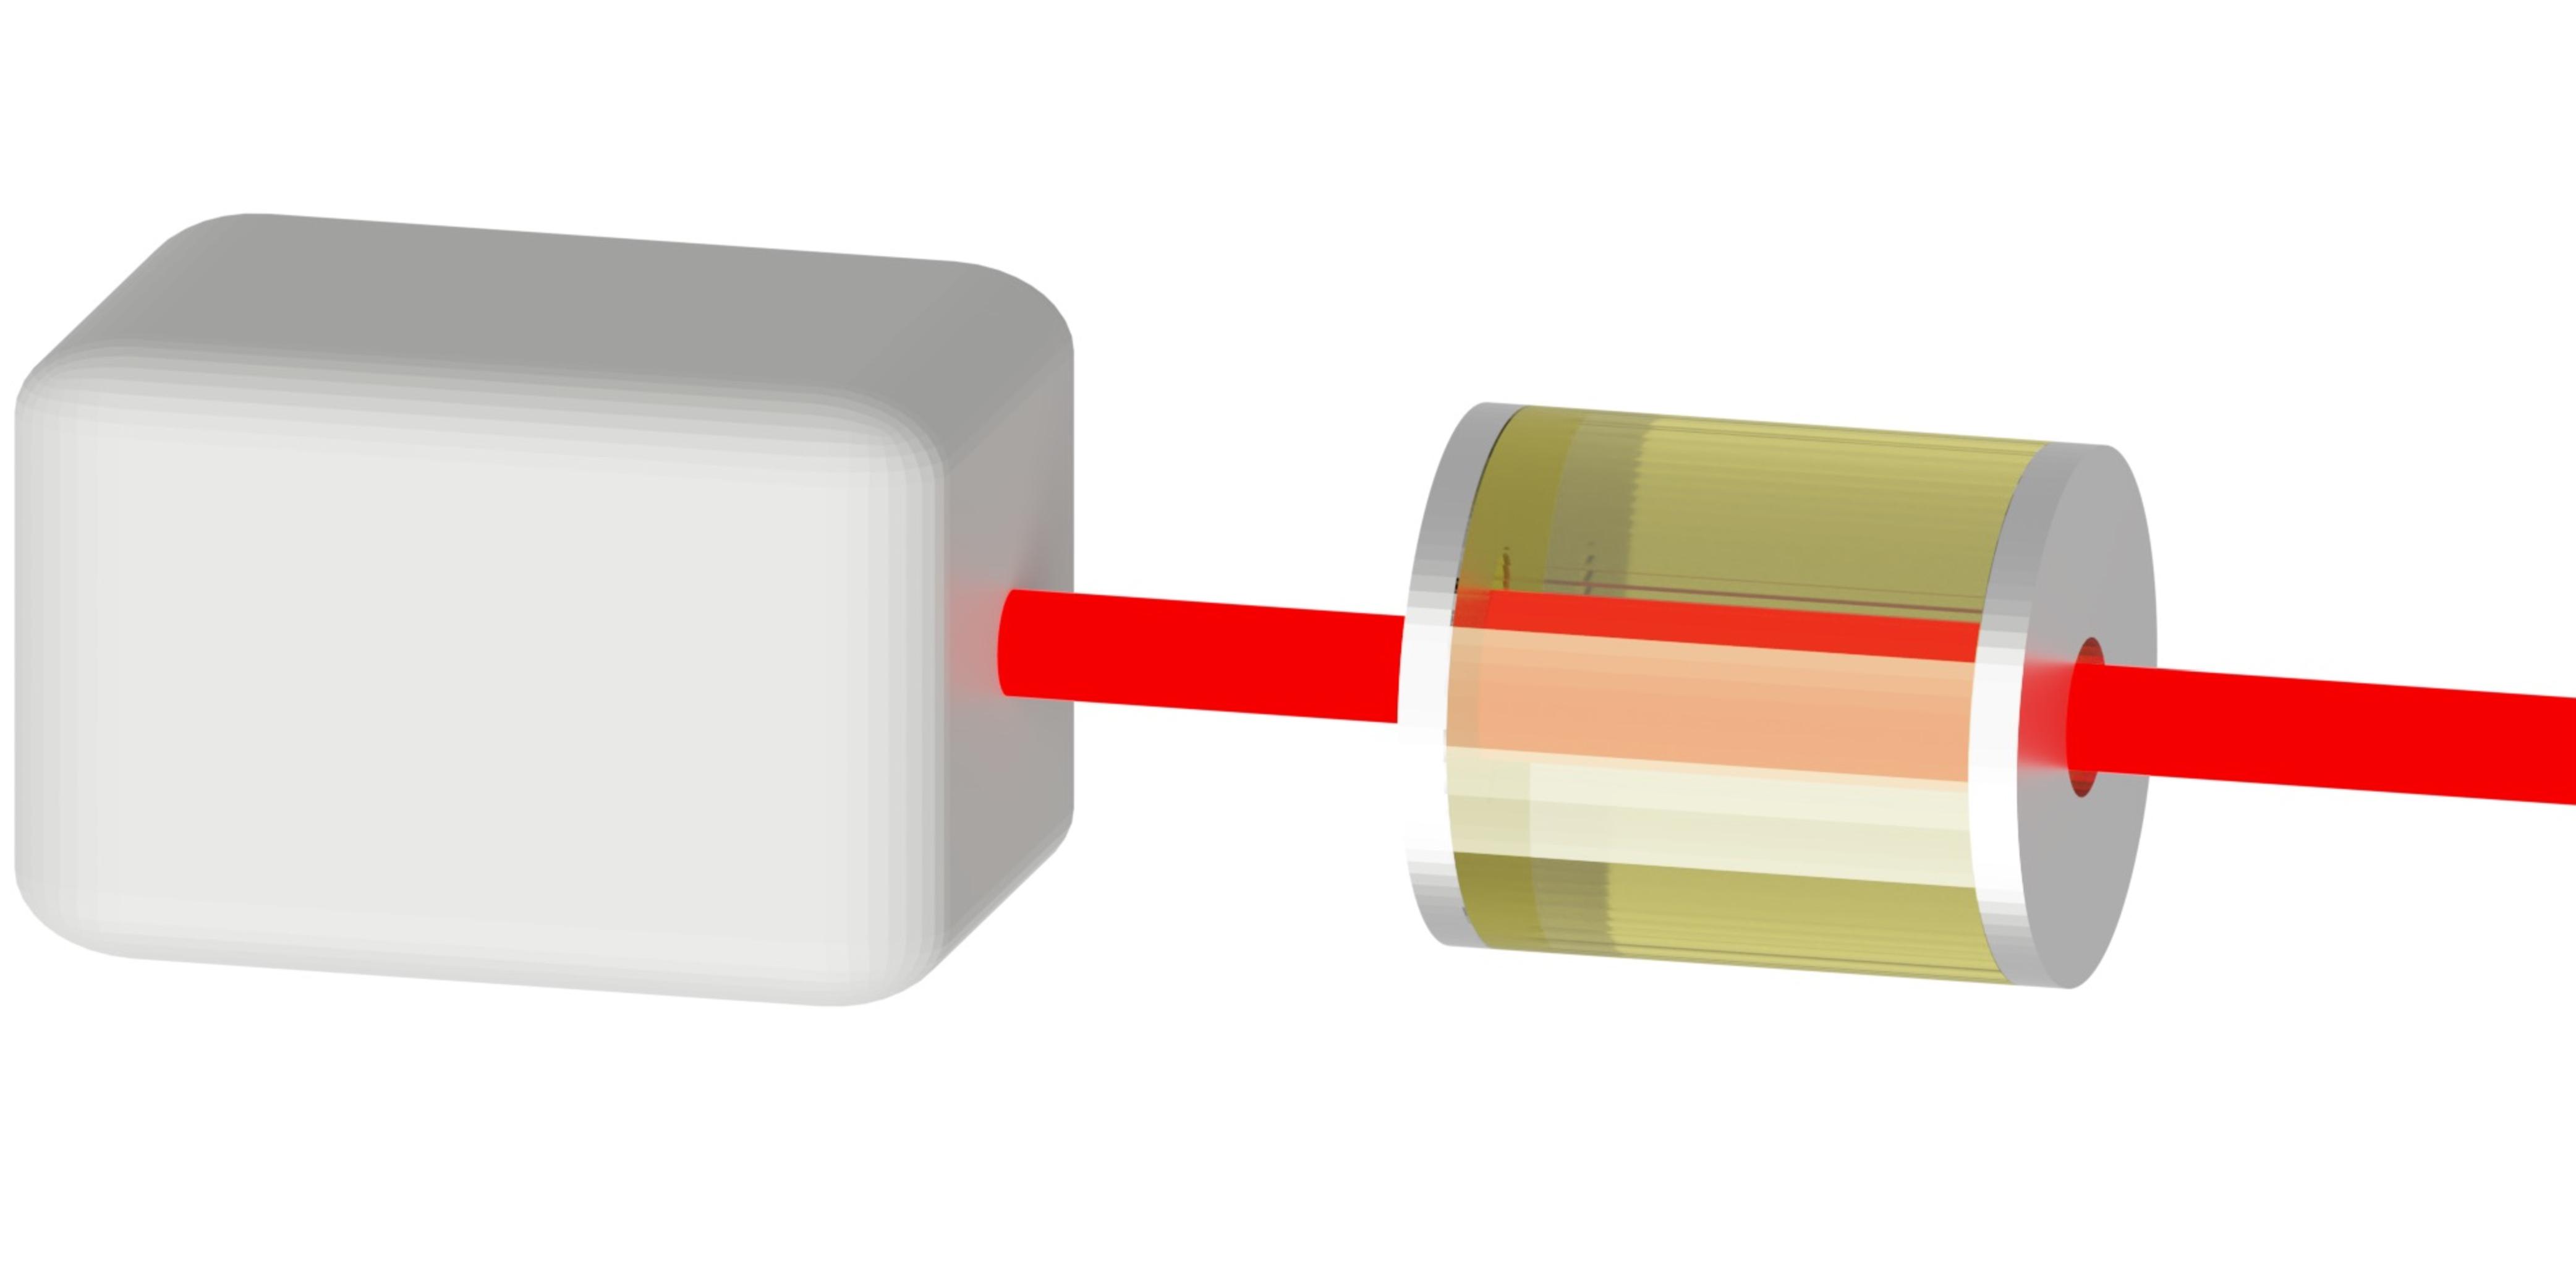
\includegraphics[width=.5\textwidth]{figs/ALGAAS/eom_l_assembly.pdf}
    \\
    \vspace{-9mm}
    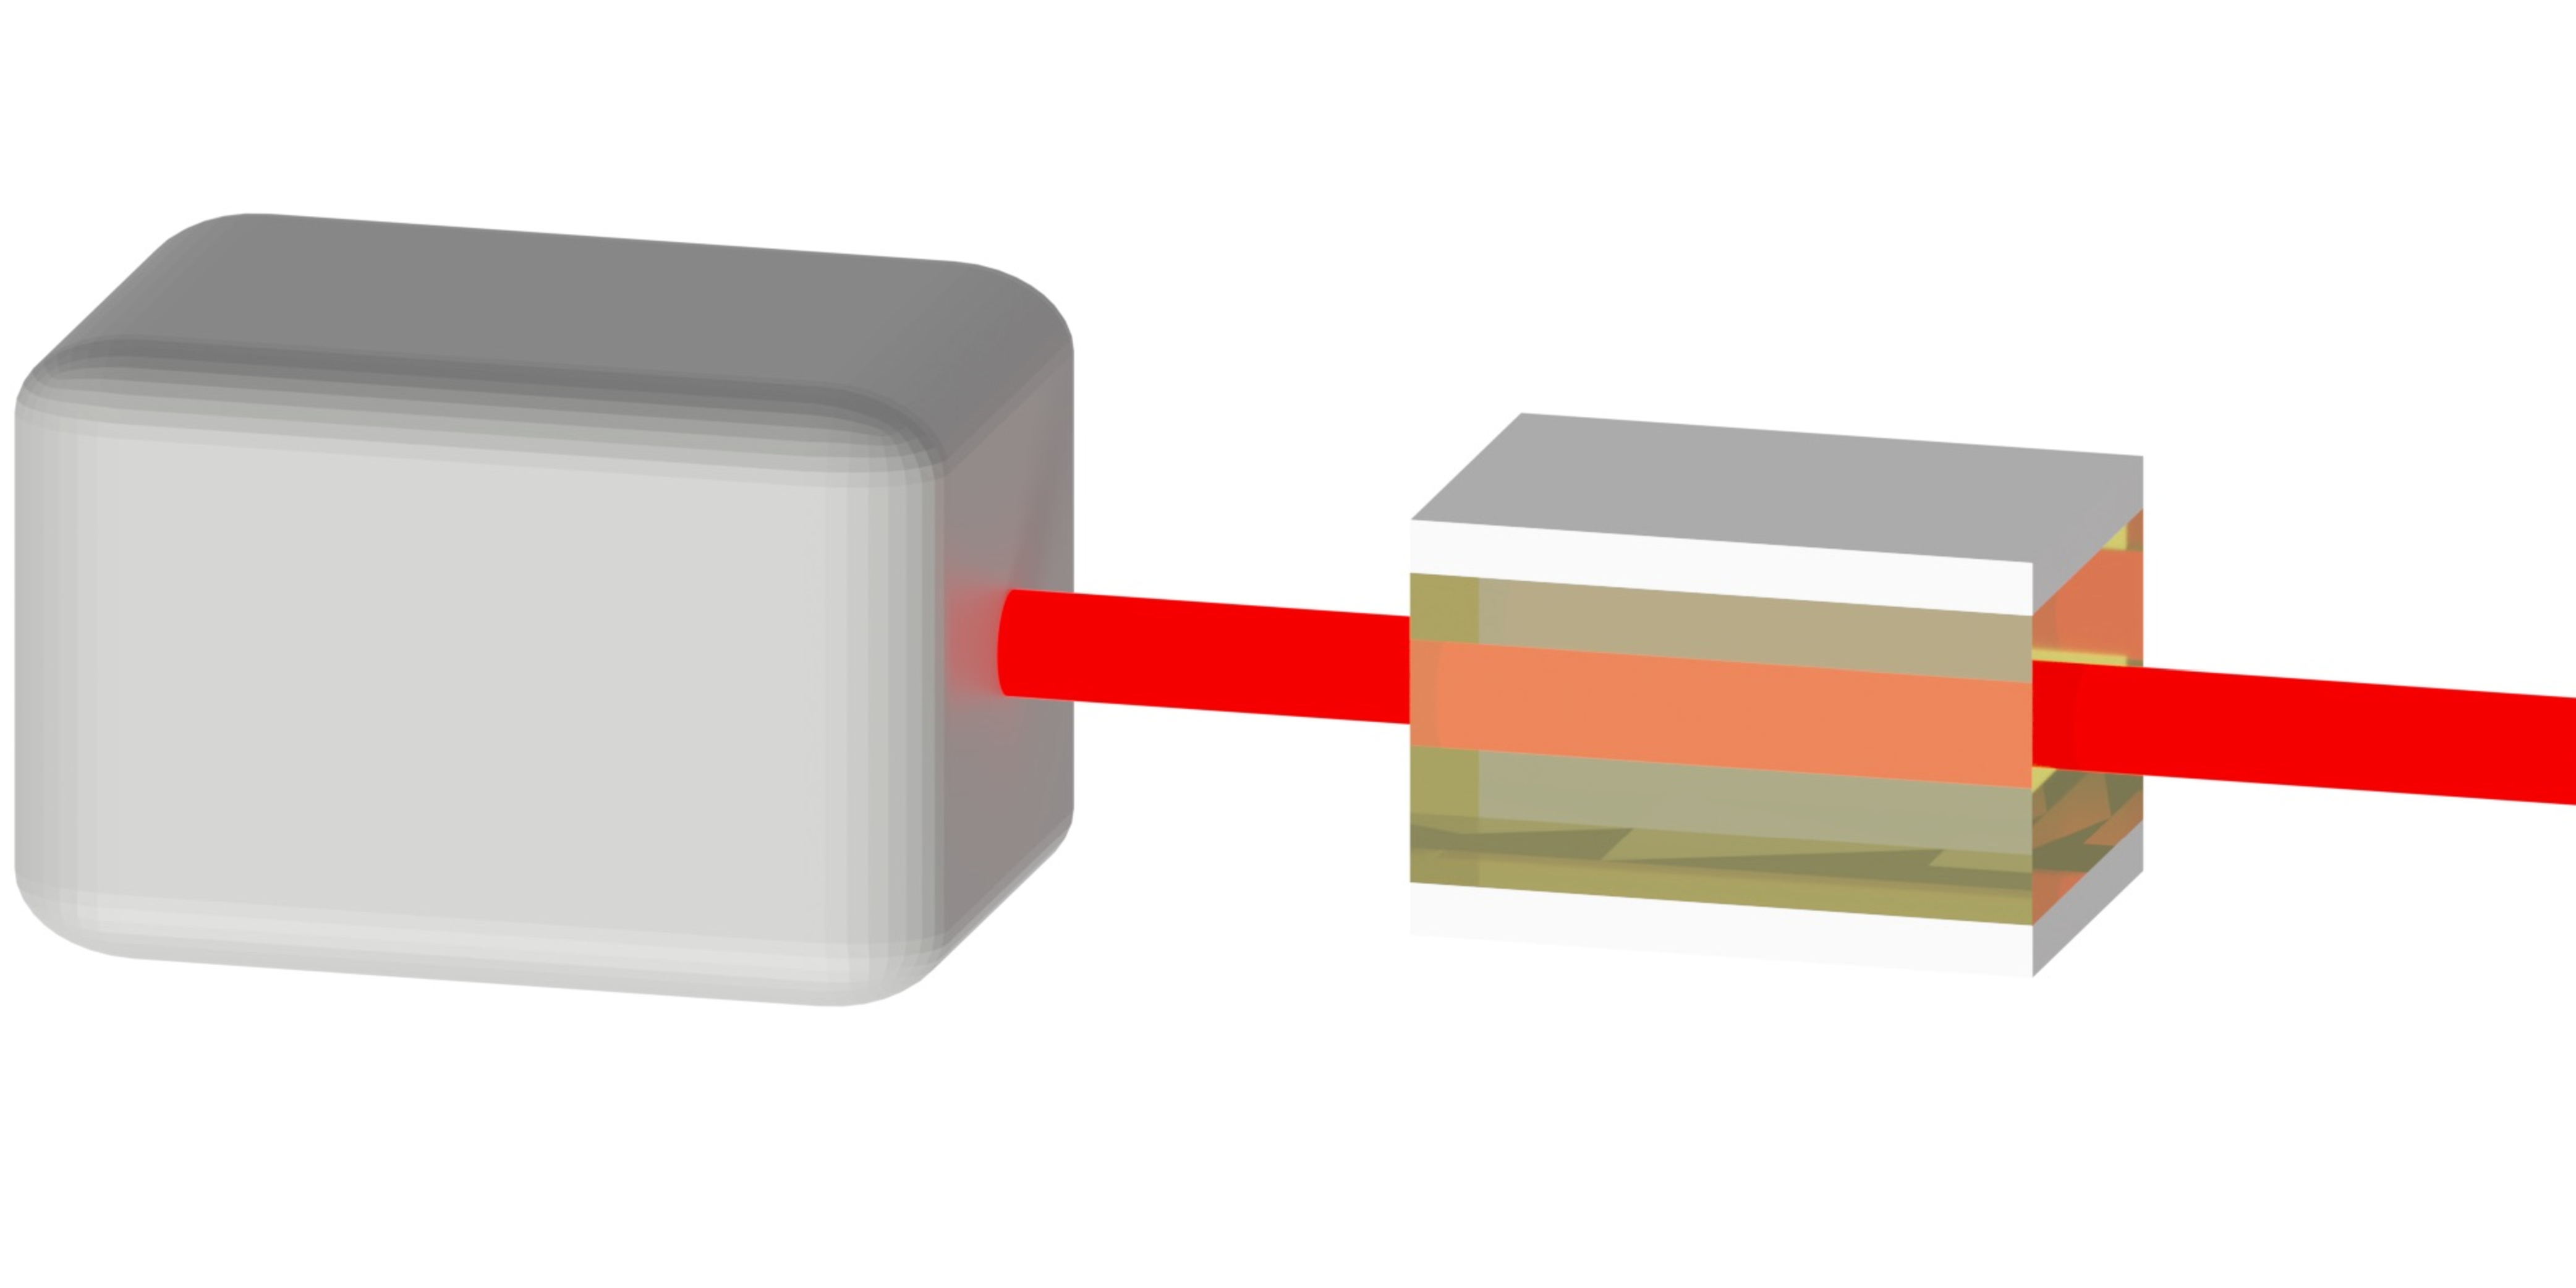
\includegraphics[width=.5\textwidth]{figs/ALGAAS/eom_t_assembly.pdf}
\caption{Longitudinal and transverse electro-optic modulators}
\label{fig:EOM_types}
\end{figure}

The voltage amplitude of the signal input is proportional to the strength of the modulated phase on the optical carrier frequency ($\omega$); commonly quantified in terms of a modulation index ($\beta$):

%%Consider a specific crystal that gives us our $\beta \mathrm{sin}(\Omega t)$

\begin{equation}\label{eq:inpEOM}
	E_\mathrm{out} = E_o e^{i \omega t + \beta \mathrm{sin}( \Omega t)} \approx E_o [J_o(\beta)e^{i \omega t} + J_1(\beta) e^{i(\omega + \Omega)t} - J_1(\beta) e^{i(\omega - \Omega)t}]  
\end{equation}

\noindent Where we have approximated with the Jacobi-Anger expansion utilizing Besssel functions of the first kind ($J_n(x)$) ~\cite{oliver:1972}:

\begin{equation}\label{eq:jacobianger}
	e^{iz \mathrm{sin}(\theta)} \approx J_0(z) + 2 \sum_{n=1}^{\infty} i^n J_n(z) \mathrm{sin} (n \theta)
\end{equation}

\ref{eq:inpEOM} sufficiently demonstrates that, to the first order, a carrier field that is phase modulated is also, in essence, imparting power to separate optical sideband fields separated in frequency by an integer multiple of the modulation $n \cdot \Omega$. Typically $\Omega$ is a chosen frequency used for optical heterodyne detection; while for a noise-driven modulation, the phase coupling is coorelated to the local directionally relevant E-field spectra alongside the propogation length of the beam propogation within the electro-optic media.

\section{Electro-optic noise of a \texorpdfstring{$\gaas$}{gaas} / \texorpdfstring{$\algaas$}{algaas} stack}
A comprehensive survey of relevant birefringent properties of a HR $\gaas$/$\algaas$ mirrorstack is due, and for this body of work includes: 1) crystal coordinate considerations when asserting an optical axis on a highly reflective crystalline stack manufactured by the Thorlabs crystalline coatings division, 2) citations of coating parameters and observed intrinsic birefringence from the highly reflective coating stack in question, 3) analysis of the differential electro-optic effect on the phase of a reflected beam, and 4) estimating the the differential phase noise in LIGO based on preliminary electric field measurements measured at LHO.

\subsection{Static Birefringence / Miller indices from a HR \texorpdfstring{$\gaas$}{gaas} / \texorpdfstring{$\algaas$}{algaas} coating}

\begin{figure}[!ht]
    \centering
	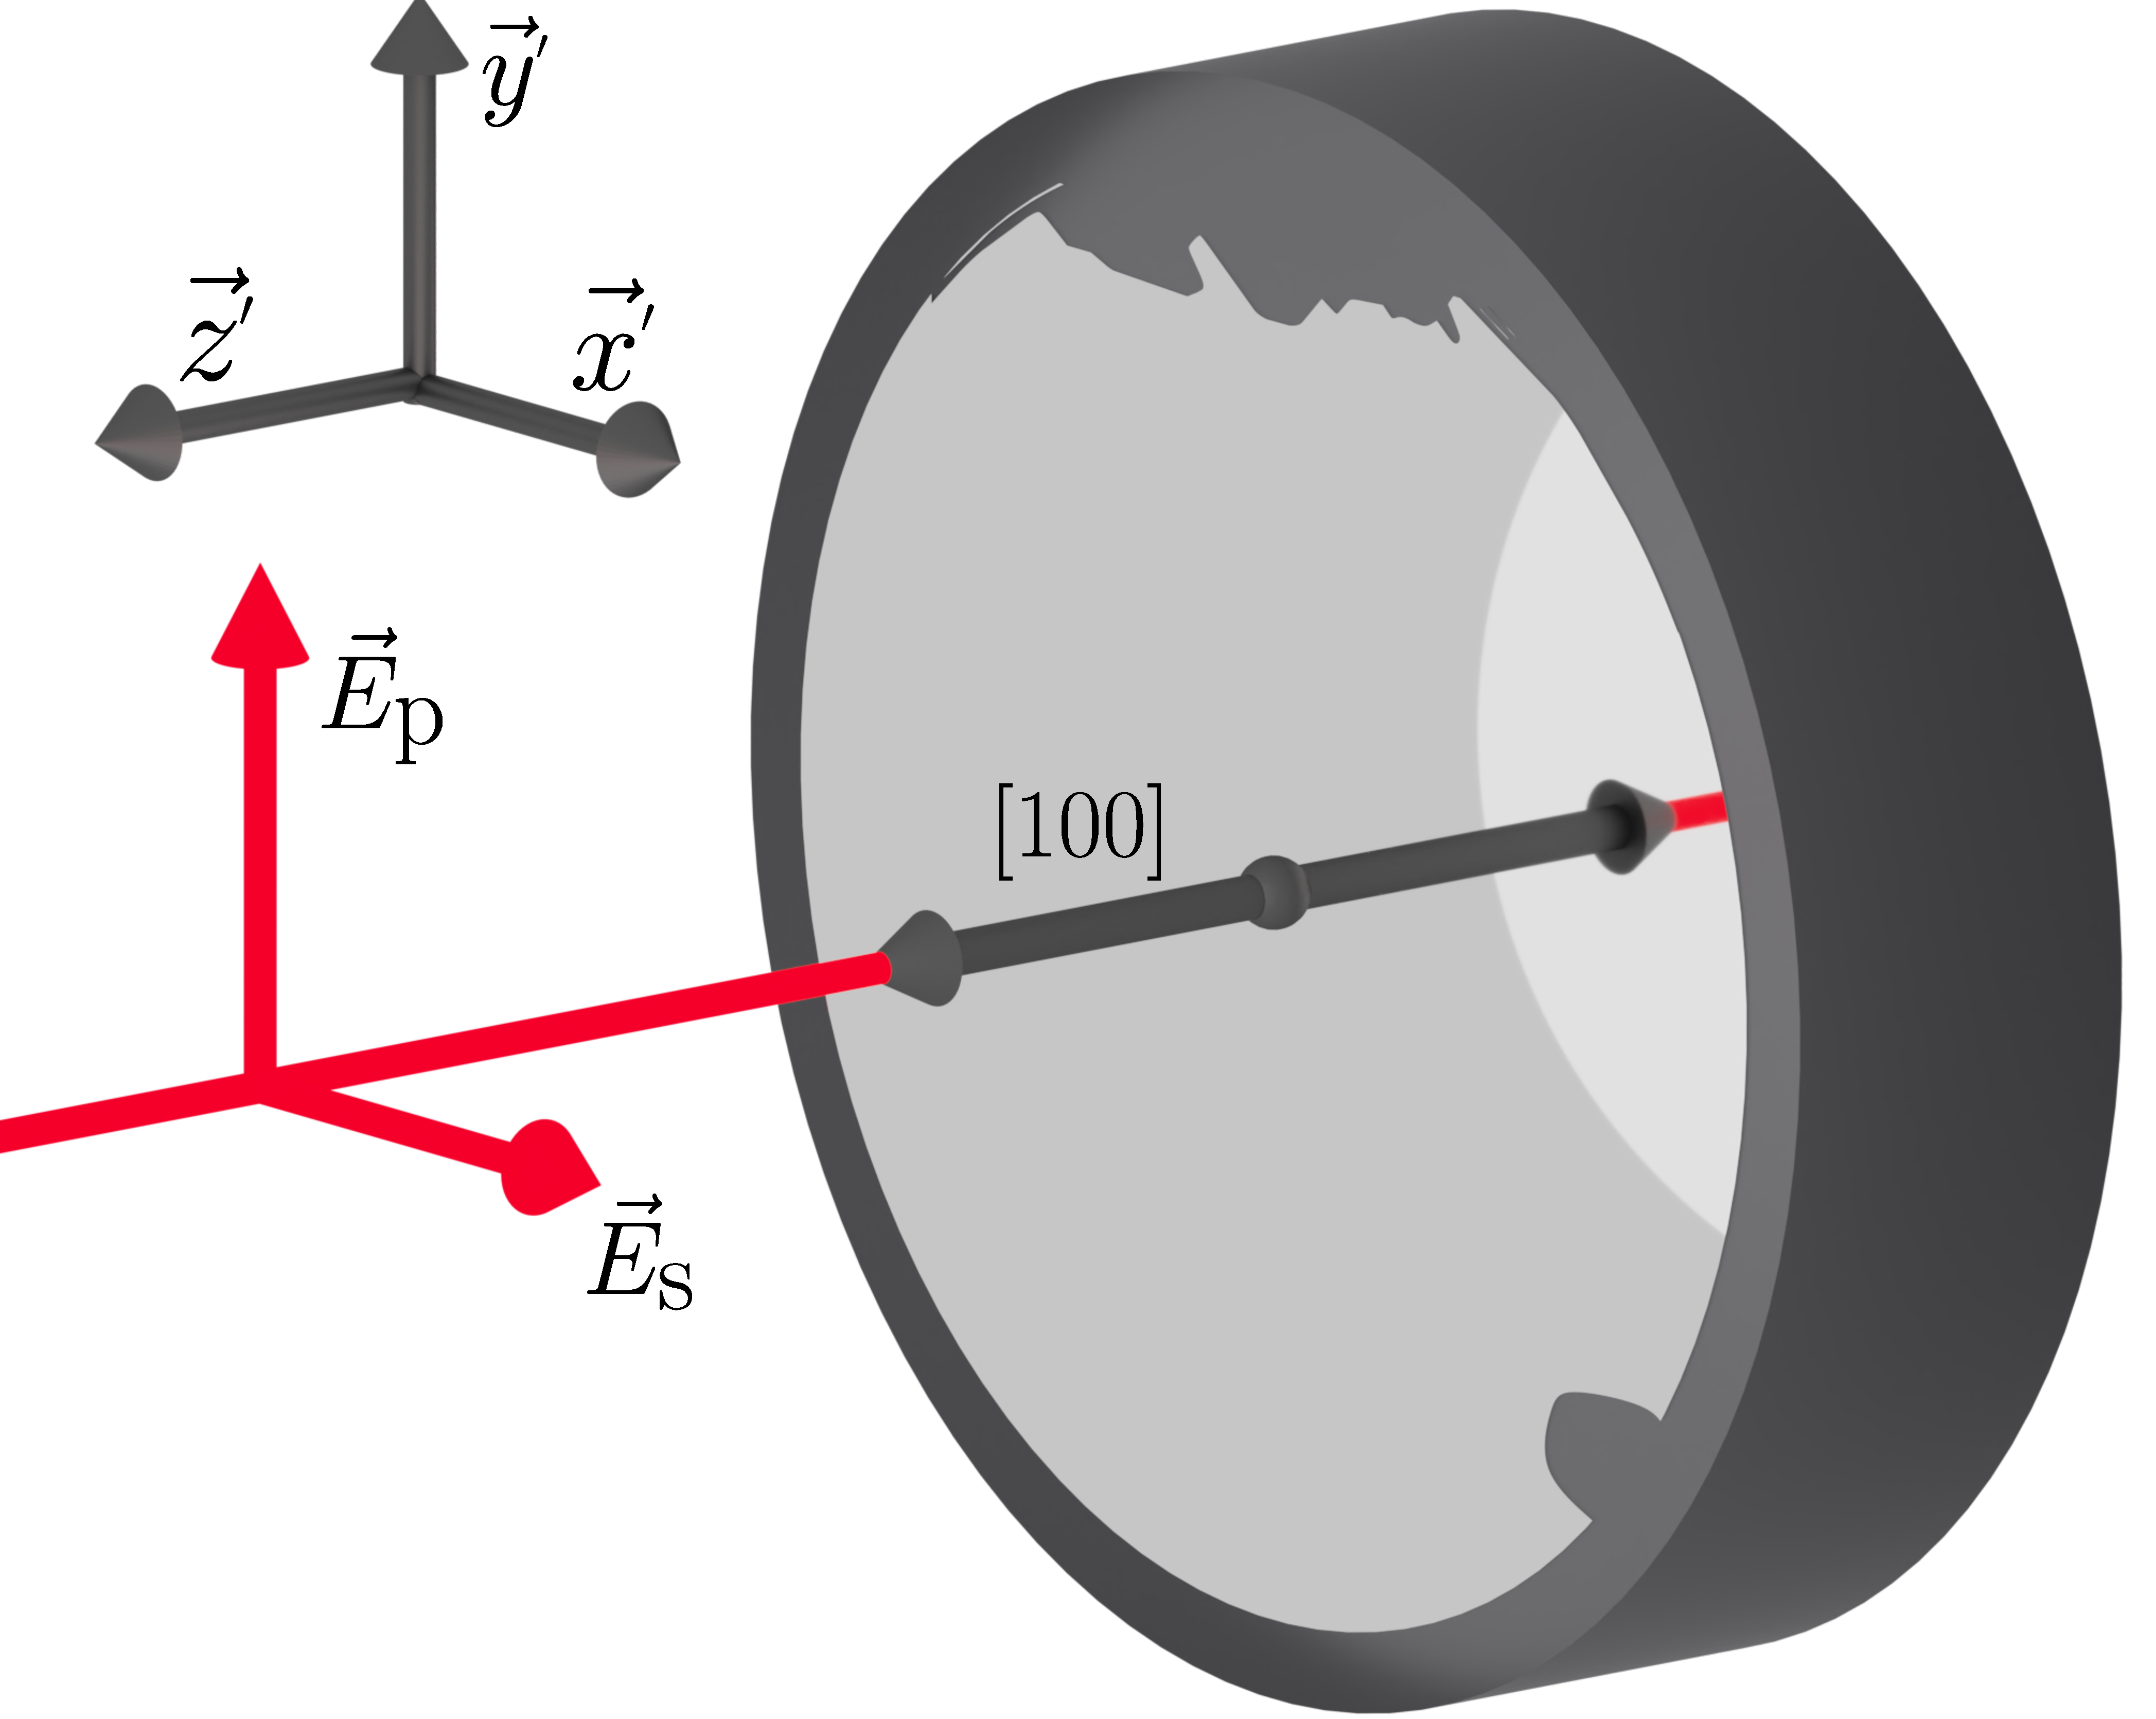
\includegraphics[width=.6\textwidth]{figs/ALGAAS/laser_mirror_algaas_coat_defect_coords.pdf}
	\caption{The beam propogation axis with respect to the $\gaas$/$\algaas$ crystal axis. The axis formed by the [100] plane normal is drawn parallel with the beam axis (z-axis) and the polarizations of incident and reflected beam oscillate along vectors within the plane formed by the normal of that axis. The topmost coordinate axis triad is drawn to depict world vectors that can help visualize the plane of computed eigenvectors. Depicted here are also defects at the top and bottom right of the coating due to overhandling but do not effect the results of this study.}
\label{fig:algaas_coord_defect}
\end{figure}



\noindent Thorlab's crystalline coatings division grows their HR crystalline optical coating such that the coating surface is drawn out in the $[100]$ plane, meaning that beam with a wavevector along the optical (z) axis draws a parallel line to the normal of said plane. Therefore since the beam's polarized E-field oscillates only within that plane, any differential splitting of the beam polarization occurs solely between rotated $[010]$ and $[001]$ axes. This allows us to restrict our interest to a field where $E_{z} \neq 0$ and $E_x = E_y =0$ and compute the eigenvalues ($\lambda^{*}_{x',y',z'}$ / eigenpolarizations ($\vec{x'}, \vec{y'}, \vec{z'}$) which lead us to the relevant eigenindices ($n_{x',y'})$ \footnote{There may appear to be an inconsistency between the miller indices and optical axes, but because of the isotropy of zincblende crystals prior to the field perturbation coordination of these axes is not quite relevant}:

\begin{equation}
    \begin{aligned}
    	\lambda_{x'} & = \big( \frac{1}{n_o ^2} - r_{41} E_z \big) \\
	\lambda_{y'} & = \big( \frac{1}{n_o ^2} + r_{41} E_z \big) \\
	\lambda_{z'} &  = \frac{1}{n_o ^2}
    \end{aligned}
\end{equation}

\noindent And the principal axes / eigenpolarizations are found when solving for the eigenvectors:

\begin{equation}
    \begin{aligned}
	\vec{x'} & = \frac{1}{\sqrt{2}}\;(0, -1, 1) \\ 
	\vec{y'} & = \frac{1}{\sqrt{2}}\;(0, 1, 1) \\
	\vec{z'} & = (1, 0, 0) \\
    \end{aligned}
\end{equation}

\begin{equation}
    \lambda_{x'}\; x'^2 + \lambda_{y'}\; y'^2 + \lambda_{z'}\; z'^2 =1
\end{equation}

\noindent The eigenindices ($n_\alpha = n_{x'}$, $n_\beta = n_{y'}$) are therefore:

\begin{equation}
    \begin{aligned}
	n_{x'} & = \sqrt{\lambda_{x'}} & = \sqrt{\frac{1}{n_o ^2} - r_{41} E_z} \\
	n_{y'} & = \sqrt{\lambda_{y'}} & =  \sqrt{\frac{1}{n_o ^2} + r_{41} E_z}
    \end{aligned}
\end{equation}



\noindent And with $n_o r_{41} E_z << 1$:

\begin{equation}
    \begin{aligned}
	n_{x'} & \approx  n_o + \frac{1}{2} n_o^3 r_{41} E_z \\
	n_{y'} & \approx n_o - \frac{1}{2} n_o^3 r_{41} E_z    
    \end{aligned}
\end{equation}

\subsection{Electro-optic coupling to the reflected phase of a HR mirror coating}
%With our chosen beam axis, the influence of an isotropic white noise field ($E_N = [E_{Nx},E_{Ny},E_{Nz}]$) is considered:

%\begin{equation}
% \left[ {\begin{array}{ccc}
%   \big( \frac{1}{n_o ^2} \big)& r_{41}E_{Ny} & r_{41} E_{Nx}\\
%   r_{41}E_{Ny} & \big( \frac{1}{n_o ^2} \big) & r_{41} E_{Nz}\\
%   r_{41} E_{Nx} & r_{41} E_{Ny} & \big( \frac{1}{n_o ^2} \big)\\
%  \end{array}} \right]
%\end{equation}

%\noindent Assuming $E_N$ is small, the indicatrix change of $E_{Nx}$ and $E_{Ny}$ relative to $E_{Nz}$ (as seen by the beam polarization) will be small ($r_{41}E_{N(x/y)} \ll r_{41}E_{Nz}$). After diagonalizing with relevant terms \footnote{Note that the form of the tensor is still in the crystal coordinates but the $E_n$ terms are placed in the tensor such that their directions align with beam axis coordinates.} in the tensor, we are left with the following eigenindices:
%
%\begin{equation}
%\begin{aligned}
%n_x' & = n_o - r_{41}E_{Nz} \\
%n_y' & = n_o + r_{41}E_{Nz}
%\end{aligned}
%\end{equation}

%How the modulation of the phase of the carrier field is dependent on the orientation of its wave vector with respect to the crystal structure, the modulating electric field direction and strength, (other items to discuss in terms of introducing the effect)
%% For GaAs @ $10.6\mu$ $r_{41} = 1.6 \times 10^{-12}$ [m/V]
%% Adachi estimate for $\mathrm{Al_{x}Ga_{1-x}As}$?
%% Relevant eigenpolarizations, non-optical field $E_y = E_z = 0$?}
%% FIGURE: SUB1 Transformed indicatrix (Before and after $E_x$)
%% FIGURE: SUB2 Ellipse cross section. New eigenpolarizations and corresponding indices and their influence on incident field (Marty's result)

\subsubsection*{Analytic estimate}
Fejer and Bonilla takes on an analytical approach to finding the impact of the electric field to the change in phase of the light through a crystalline anisotropic thin film ($\lambda/4$) stack. The construction builds off of a pre-defined defivation of thermo-optic noise calculations for the HR stack and assuming a large enough number of high-low index coating pairs~\cite{bonillafejer, fejer_estimate}:

\begin{equation}
    \bigg| \frac{\partial \phi}{\partial E} \bigg| = - \pi \frac{r_{41}}{2}(n_\mathrm{high} n_\mathrm{low} ^2 + n_\mathrm{low} n_\mathrm{high} ^2) \frac{n_\mathrm{high}}{n_\mathrm{low}}
\end{equation}

With $n_\mathrm{low} = n_\algaas = 2.9369$, $n_\mathrm{high} = n_\gaas = 3.4786$, and $r_{41} = -1.33 \times 10^{-12}$

The estimated differential phase from the electro-optic effect with a 1064nm E-field propogating along the [110] axis of the HR $\gaas / \algaas$ stack:

$$
\bigg| \frac{\partial \phi}{\partial E} \bigg| = 4.0253 \times 10^{-12} \; \frac{[\mathrm{rad}]}{[\mathrm{V}/\mathrm{m}]}
$$
%\begin{equation}
%\hat{\phi}' = \frac{\pi n_1 z}{1-z^2}(z^{2N} -1) \frac{z^{2N} \frac{(n_f)^2}{n_2 n_3}(n_2 \kappa_{\gamma 2} + n_3\kappa_{\gamma 3}) - (n_2 \kappa_{\gamma 3} + n_3\kappa_{\gamma 3})}{(n_1)^2 -(n_f)^2 z^{4N}}
%\end{equation}

%with $z = \frac{n_2}{n_3}$
%and
%$
%\kappa_{\gamma j} = \frac{d}{d \gamma} \mathrm{log}(n_j h_j)|_{\gamma =\gamma_{O}} \bigg(\frac{\hat{n}_j'}{\hat{n}_j} +\frac{\hat{h}_j'}{\hat{h}_j} \bigg)
%$

With $\kappa$ being a scalar parameter.
%%FIGURE: Cross sectional view of multilayer coating

\begin{figure}[!ht]
	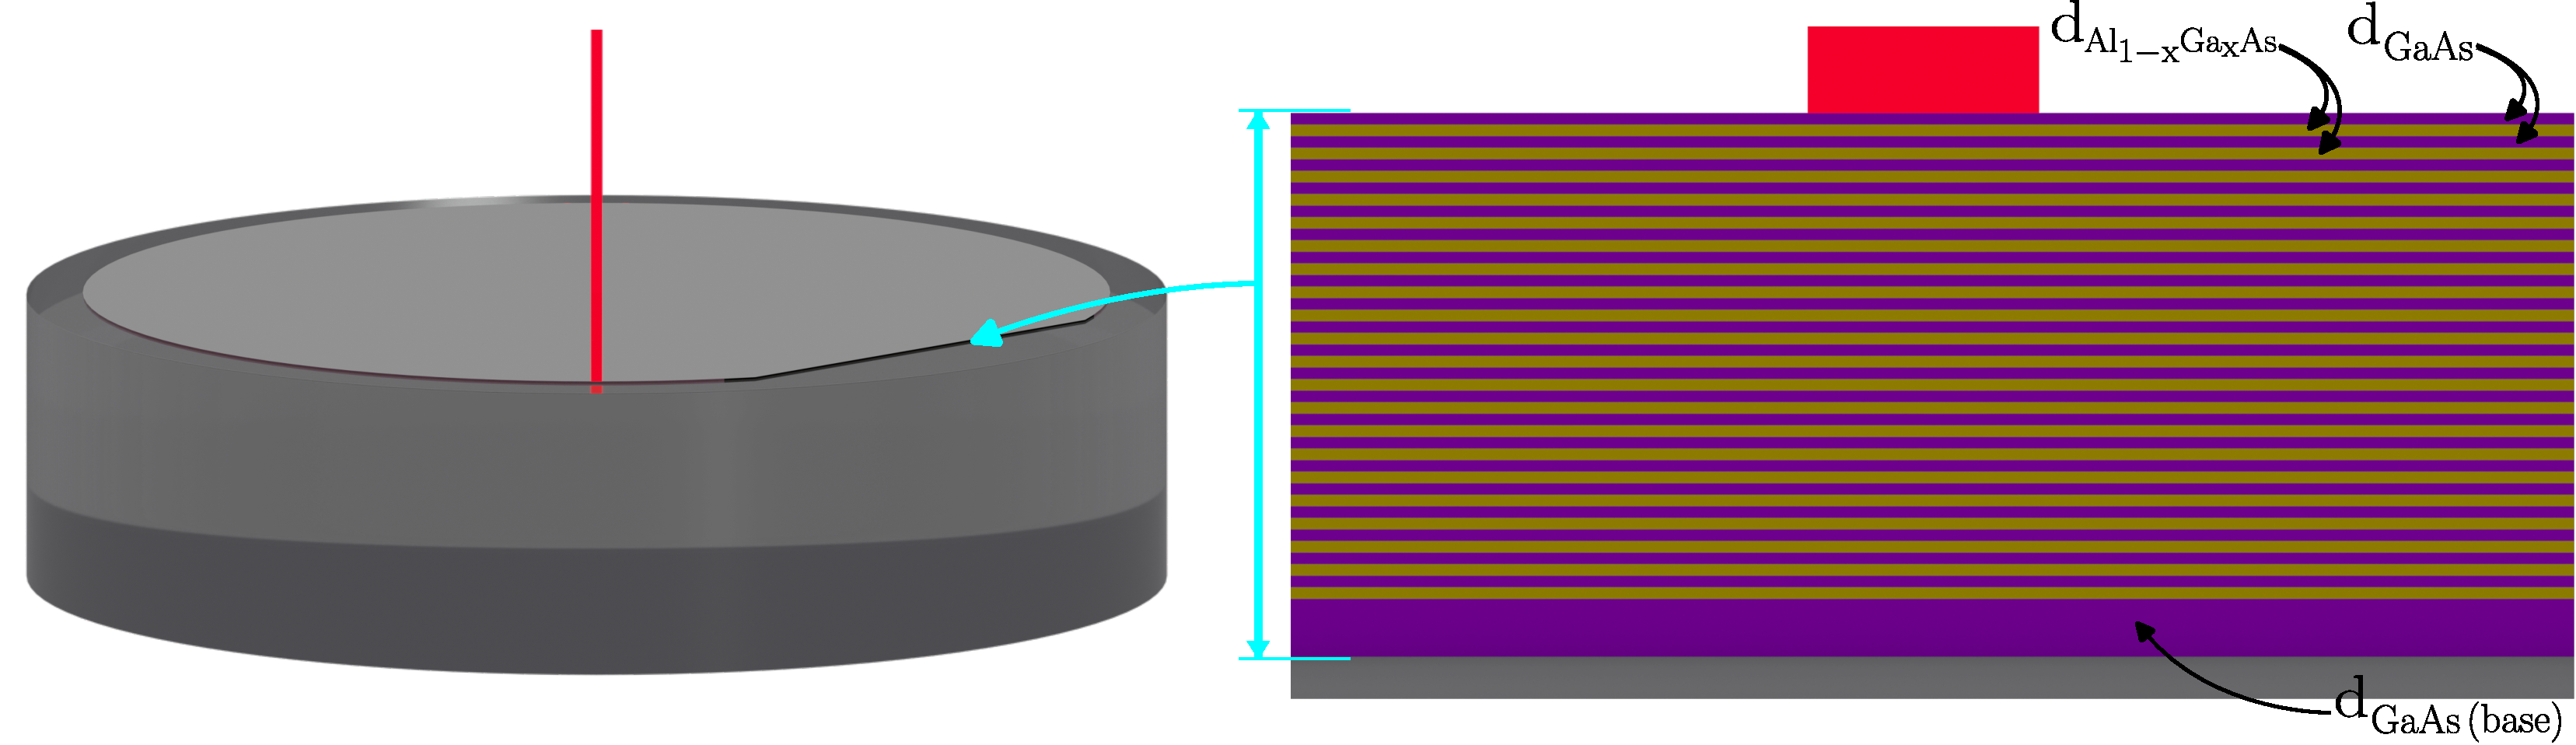
\includegraphics[width=\textwidth]{figs/ALGAAS/ALGAAS_HR_layers_ann.pdf}
\caption{The beam propogation axis ($\vec{S}$, $[-100]$) with respect to the $\gaas$/$\algaas$ crystal axes. The axis formed by the [100] plane normal is drawn parallel with the beam axis (z-axis) and the polarizations of incident and reflected beam oscillate along vectors within the plane formed by the normal of that axis. The coating is grown with a flat indicating a line within the [0-11] plane; where the plane normal points towards the sample center.}
\label{fig:HRlayers}
\end{figure}


\subsubsection*{Numerical estimate}

In the appendix of \cite{ballmer:2015} Ballmer constructs a coating layer transfer function for a given coating layer k with index $n_k$, and thickness $d_k$, defining right and left propogating modes $\psi^{R,L}$ repsectively:
$$
  \left[ {\begin{array}{c}
   \psi^\mathrm{R} \\
   \psi^\mathrm{L} \\
  \end{array} } \right]_{k+1}
  =
%
Q_k D_k
%
 \left[{\begin{array}{c}
   \psi^\mathrm{R} \\
   \psi^\mathrm{L} \\
 \end{array}} \right]
$$
\noindent $D_k$ applies the phase ($\phi_k = 4\pi n_k d_k /\lambda_0$) from a given coating layer, and $Q_k$ applies the transfer function between high-low/low-high index layers transition:

\begin{equation}
D_k =
\left[ {\begin{array}{cc}
  e^{-i \phi_k / 2}& 0\\
 0 & e^{i \phi_k / 2}\\
\end{array} } \right]
\end{equation}

\begin{equation}
Q_k = \frac{1}{2n_{k+1}}
\left[ {\begin{array}{cc}
  n_{k+1} + n_k & n_{k+1} - n_k\\
 n_{k+1} - n_k & n_{k+1} + n_k\\
\end{array} } \right]
\end{equation}
\noindent Defining a HR coating stack, the total transfer matrix from vaccum $Q_0$ to the $N$th coating layer is:
\begin{equation}
	M = Q_N D_N ...Q_k D_k...Q_1D_1Q_0
\end{equation}
\noindent And the partial derivative at the kth coating layer is:

\begin{equation}
	\label{eq:partialM}
	\frac{\partial M}{\partial \phi_k} = Q_N D_N ...Q_{k} \begin{bmatrix} e^{-i \phi_k /2} & 0 \\ 0 & e^{i \phi_k/2} \end{bmatrix} \begin{bmatrix} -i /2 & 0 \\ 0 & i/2 \end{bmatrix} Q_{k-1} D_{k-1}...Q_1D_1Q_0
\end{equation}

\noindent The above representing a collective differential phase manifesting as a sum of these phase components. This explicit perturbed phase at the kth layer for the electro-optic effect ($\partial n_k/\partial E$) is found when:
\begin{equation}\label{eq:EOphasekdiff}
	\frac{\partial \phi_k}{\partial E} = \frac{4 \pi d_k}{\lambda} \frac{\partial n_k}{\partial E} = \pm \frac{ 2 \pi}{\lambda} n_k^3 d_k r_{41,k}
\end{equation}
\noindent Where the electro-optic coefficients $r_{41}$ for $\gaas$ and $\algaasgen$ \cite{suzuki:1984, adachi:2012, adachi:1985}:
\begin{equation}
\begin{aligned}
	& r_{41, \gaas} =  -1.33 \times 10^{-12} & [\mathrm{m} / \mathrm{V}]
	\\ 
	& r_{41, \algaasgen}  = - (1.33 - 0.45x) \times 10^{-12} &  [\mathrm{m}/\mathrm{V}]
\end{aligned}
\end{equation}
\noindent Rather than tagging on the phases individually, an easier computation is found when relying on the relationship between the transmission ($t$) and reflectivity ($r$) to a general transfer matrix (in our case $M$):
$$
	\begin{bmatrix} 1 \\ r \end{bmatrix} \begin{bmatrix} M_{11} & M_{12} \\ M_{21} & M_{22} \end{bmatrix} = \begin{bmatrix} t \\ 0\end{bmatrix}
$$
\noindent And using this relation, differentiating the reflectivity with respect to $\phi_k$:
$$
	\frac{\partial r}{\partial \phi_k} = - \bigg( \frac{1}{M_{21}} \frac{\partial M_{21}}{\partial \phi_k} - \frac{1}{M_{22}}\frac{\partial M_{22}}{\partial \phi_k} \bigg) \frac{M_{21}}{M_{22}}
$$
\noindent The differential reflectivity is normalized by the total reflectivity and taking the imaginary component as noted in~\autoref{eq:partialM}: 

\begin{equation}
	\frac{\partial \phi_c}{\partial \phi_k}  = \mathrm{Im} \bigg(\frac{1}{r} \frac{\partial r}{\partial \phi_k} \bigg) =  \bigg( \frac{1}{M_{21}} \frac{\partial M_{21}}{\partial \phi_k} - \frac{1}{M_{22}}\frac{\partial M_{22}}{\partial \phi_k} \bigg) 
\end{equation}

\noindent The impact of a differential electric noise field ($E_\mathrm{STLF}$) on $M$ due to the electro-optic effect on the kth layer, we use the chain rule:

\begin{equation}
	\bigg| \frac{\partial \phi_c}{\partial  E_\mathrm{STLF}} \bigg| =  \bigg| \frac{\partial \phi_c}{\partial \phi_k}  \frac{\partial \phi_k}{\partial E} \bigg|
\end{equation}

The coating to be studied consists of 36 $\lambda$/4  thick layers of $\gaas$ interspersed with 35 layers of $\lambda$/4 thick $\algaas$. $\gaas$ forms the top and bottom layer to prevent oxygen absorption from the AlGaAs layer. The $\gaas$ layers have an index of $n_{\gaas} = 3.480$ and a thickness of $\Delta d_{\gaas} = 76.43$ nm while the low index $\algaas$ layers are $n_{\algaas} = 2.977$ with thickness $\Delta d_{\algaas} = 89.35$ nm. With the constructed matrices, we apply these parameters and compute a differential phase of:

\begin{equation}
    \bigg| \frac{\partial \phi_c}{\partial  E_\mathrm{STLF}} \bigg|  = 3.9 \times 10^{-11}\; \frac{[\mathrm{rad}]}{[\mathrm{V}/\mathrm{m}]}     
\end{equation}

%High Index:  GaAs, n=3.480, layer thickness is 76.43 nm
%Low Index:  $ \mathrm{Al}_{0.92} \mathrm{Ga}_{0.08} \mathrm{As} $, n=2.977, layer thickness is 89.35 nm
%Info from Steve. Written source

%% Marty's document about Birefringence in Crystalline mirror coatings V.8

\subsection{Initial projected DARM coupling}
Measured field spectra acquired from installed electric field meters located within LHO and LLO ETMX and ETMY vacuum chambers can help translate how much DARM coupling can occur from electro-optic coating noise. For O3 the EFMs were located next to the test mass mirrors and measured a consistent 3 $[\mu \mathrm{V} / \mathrm{m} / \sqrt{\mathrm{Hz}}]$ @ 100 Hz~\cite{buikema:2020}. This along with computed estimate allows us to create an upper limit for what this noise might be assuming incoherent fields between the end stations and a flat frequency response within LIGO's bandwidth. An initial differential phase noise estimate of $\approx 4.5\times 10^{-10}$ [rad/m/V], alongside measured LHO ambient field noise measured during O3 we compute an initial strain noise estimate ~\cite{fejer_estimate, buikema:2020}:

\begin{equation*}
    \frac{\partial L}{\partial E} = \frac{\lambda}{4 \pi} \bigg| \frac{\partial \theta_c}{\partial E} \bigg| = 3.81 \times 10^{-17} \; \frac{[\mathrm{m}]}{[\mathrm{V/m}]}
\end{equation*}

\begin{equation}
    h_\mathrm{EO\; noise} = 2\frac{\Delta L_\mathrm{EO \; noise}}{L} = 2\frac{\partial L}{\partial E} \times \bigg| \frac{E_\mathrm{noise}}{L_\mathrm{arm}} \bigg| = 5.715 \times 10^{-26} \; \mathrm{[Hz]}
\end{equation}



% Taking the upper and the lower EFM measurements from ~\cite{efmlog} $.3\; [\mathrm{V}/\mathrm{m}/\sqrt{\mathrm{Hz}]}$ @ 60 Hz and $4\times10^{-3}\; [\mathrm{V}/\mathrm{m}/\sqrt{\mathrm{Hz}]}$ @ 4kHz.
%% \satoshi{I don't think these values are calibrated. According to Martynov et al. 2016, the fluctuations in the electric filed is $\sim10^{-5}\,\mathrm{[(V/m)/\sqrt{Hz}]}$.}

\section{Electro-optic measurement apparatus}
In seeking a calibrated estimate of the electro-optic effect for the $\gaas$/$\algaas$ mirror coating stack, we sought to drive an electro-optic response of a mirror sample from Thorlab's crystalline mirror coatings division placed within a custom longitudinal Pockels cell mirror mount. The assembly, with the installed sample, assumed the end mirror position within a two mirror Fabry-Perot cavity, while resonance of a circulating Nd:YAG 1064nm carrier beam was held by a Pound-Drever-Hall servo. As seen in the prior section, the size of the imparted phase noise for currently existing gravitational wave detector configurations is estimated to be small but notable. Investigation through measurement of said effect requires detection methods with sufficient sensitivity for the differential phase noise imparted by the effect. Details and specifications of the detection schema are discussed along with relevant measurements and results. 

%% Driven acoustic modes of the longitudinal pockels cell mirror mounts lead to numerous mounting strategies that will be detailed below. 


\begin{figure}[H]
	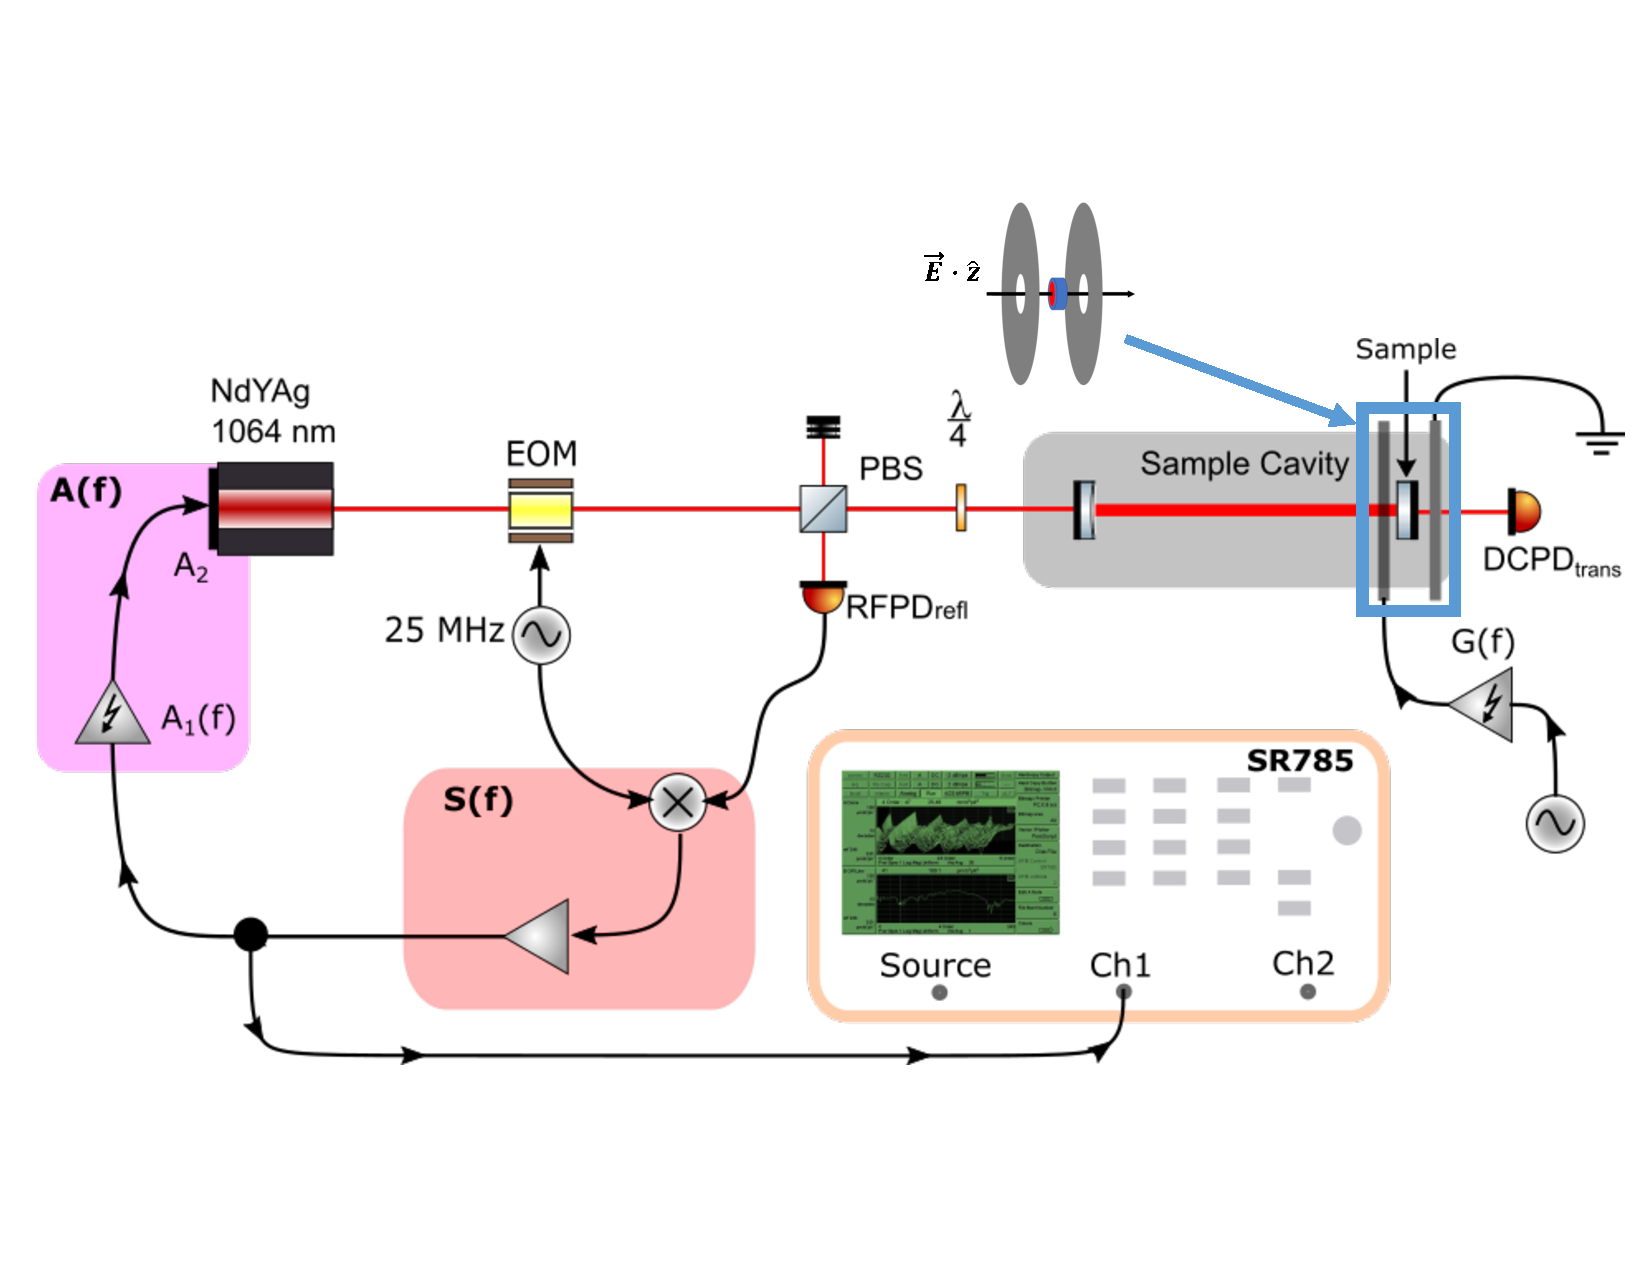
\includegraphics[width=\textwidth]{figs/ALGAAS/algaas_pockels_effect_measurement_schematic.pdf}
	\caption{A simplified and modular schematic of the PDH servo used along with an electrostatic drive mount design comprised of a disk capacitor sandwiching the HR AlGaAs sample, a high voltage amplifier, and a signal / network analyzer.}
\label{fig:simpschema}
\end{figure}
 Measurability of the electro-optic effect is contingent upon two initial design criteria: the sensitivity of the optical plant to be implemented in the PDH servo, and the maximum achievable electric field strength along the beam axis ($|E_z|_\mathrm{max}$).

\subsection{PDH servo}\label{subsubsec:pdh}
The Pound-Drever-Hall technique, originally and commonly used for laser frequency stabilization to an ultra-stable length reference, allows the tracking of the linear phase response of an input carrier field through cavity resonance. The servo fully realizes the ability of an optical cavity to act as a length / frequency discriminator:

\begin{equation}\label{eq:cavlf}
	\frac{\Delta f}{f} = \frac{\Delta L}{L}
\end{equation}

\noindent The alternative side-of-fringe lock provides a linear response in intensity, which is adequate for some applications but with reduced sensitivity due to the required power reduction by operating off resonance. Measurements of phase are extracted through an optical heterodyne; the co-propogation of a separate (but phase-locked) optical field with a known frequency separation to the carrier reflected from the cavity input. The PDH servo bypasses the need for a complicated phase-locked two laser configuration by imposing a phase modulation onto the carrier field via an electro-optic modulator (aka Pockels cell) mentioned in section \autoref{sec:EOM}. Setting a photodiode of area ($A_\mathrm{PD}$) in reflection of the cavity with a coefficient of $r_\mathrm{cav}(\omega,L)$, we measure the reflected power of the input field given by \autoref{eq:inpEOM}\;:

%If the modulation depth given by \ref{eq:inpEOM} is set such that $\beta < 1$ then the input field may be approximated in terms of the first two Bessel functions $J_0$, $J_1$:

%\begin{equation} \label{eq:EOM_trans_field}
%E_\mathrm{inp} \approx E_0 [J_0(\beta)e^{i \omega t} + J_1(\beta)e^{i (\omega + \Omega) t} - J_1(\beta)e^{i(\omega -\Omega)t}]
%\end{equation}
%
%With a high enough modulation frequency the terms given above can be far enough from the carrier frequency, so that the phase modulation onto the carrier field is mathematically and physically equivalent to imposing separate optical fields (sidebands) which in most cases do not resonate in the optical cavity of interest. 



\begin{equation}
 \begin{alignedat}{3}
    &P_\mathrm{refl} && \approx \frac{|E_\mathrm{refl}|^2}{A_\mathrm{PD}} && \\
    & &&\approx \frac{E_0^2}{A_\mathrm{PD}} && \bigg\{J_0^2 |r_\mathrm{cav}(\omega,L)|^2 + J_1^2(\beta)|r_\mathrm{cav}(\omega+\Omega,L)|^2 - J_1^2(\beta)|r_\mathrm{cav}(\omega-\Omega,L)|^2 +  \\
    & && && J_0J_1(\beta)\big[r_\mathrm{cav}\omega,L) r_\mathrm{cav}^*(\omega+\Omega,L)\big] - J_ 0J_1(\beta)\big[r_\mathrm{cav}(\omega,L)r_\mathrm{cav}^*(\omega-\Omega,L)\big]\bigg\}
  \end{alignedat}
\end{equation}

The two trailing terms in the above equation for $P_\mathrm{refl}$ generate a beat frequency term between the carrier and lower and upper sidebands. The magnitude and sign of these beat terms directly relate to the phase of the reflected carrier field and can be measured and transformed to the error signal seen in \autoref{fig:pdherr} using resonant electronics (tuned to a chosen sideband frequency) for amplification and a mixer for demodulation.

\begin{figure}[H]
	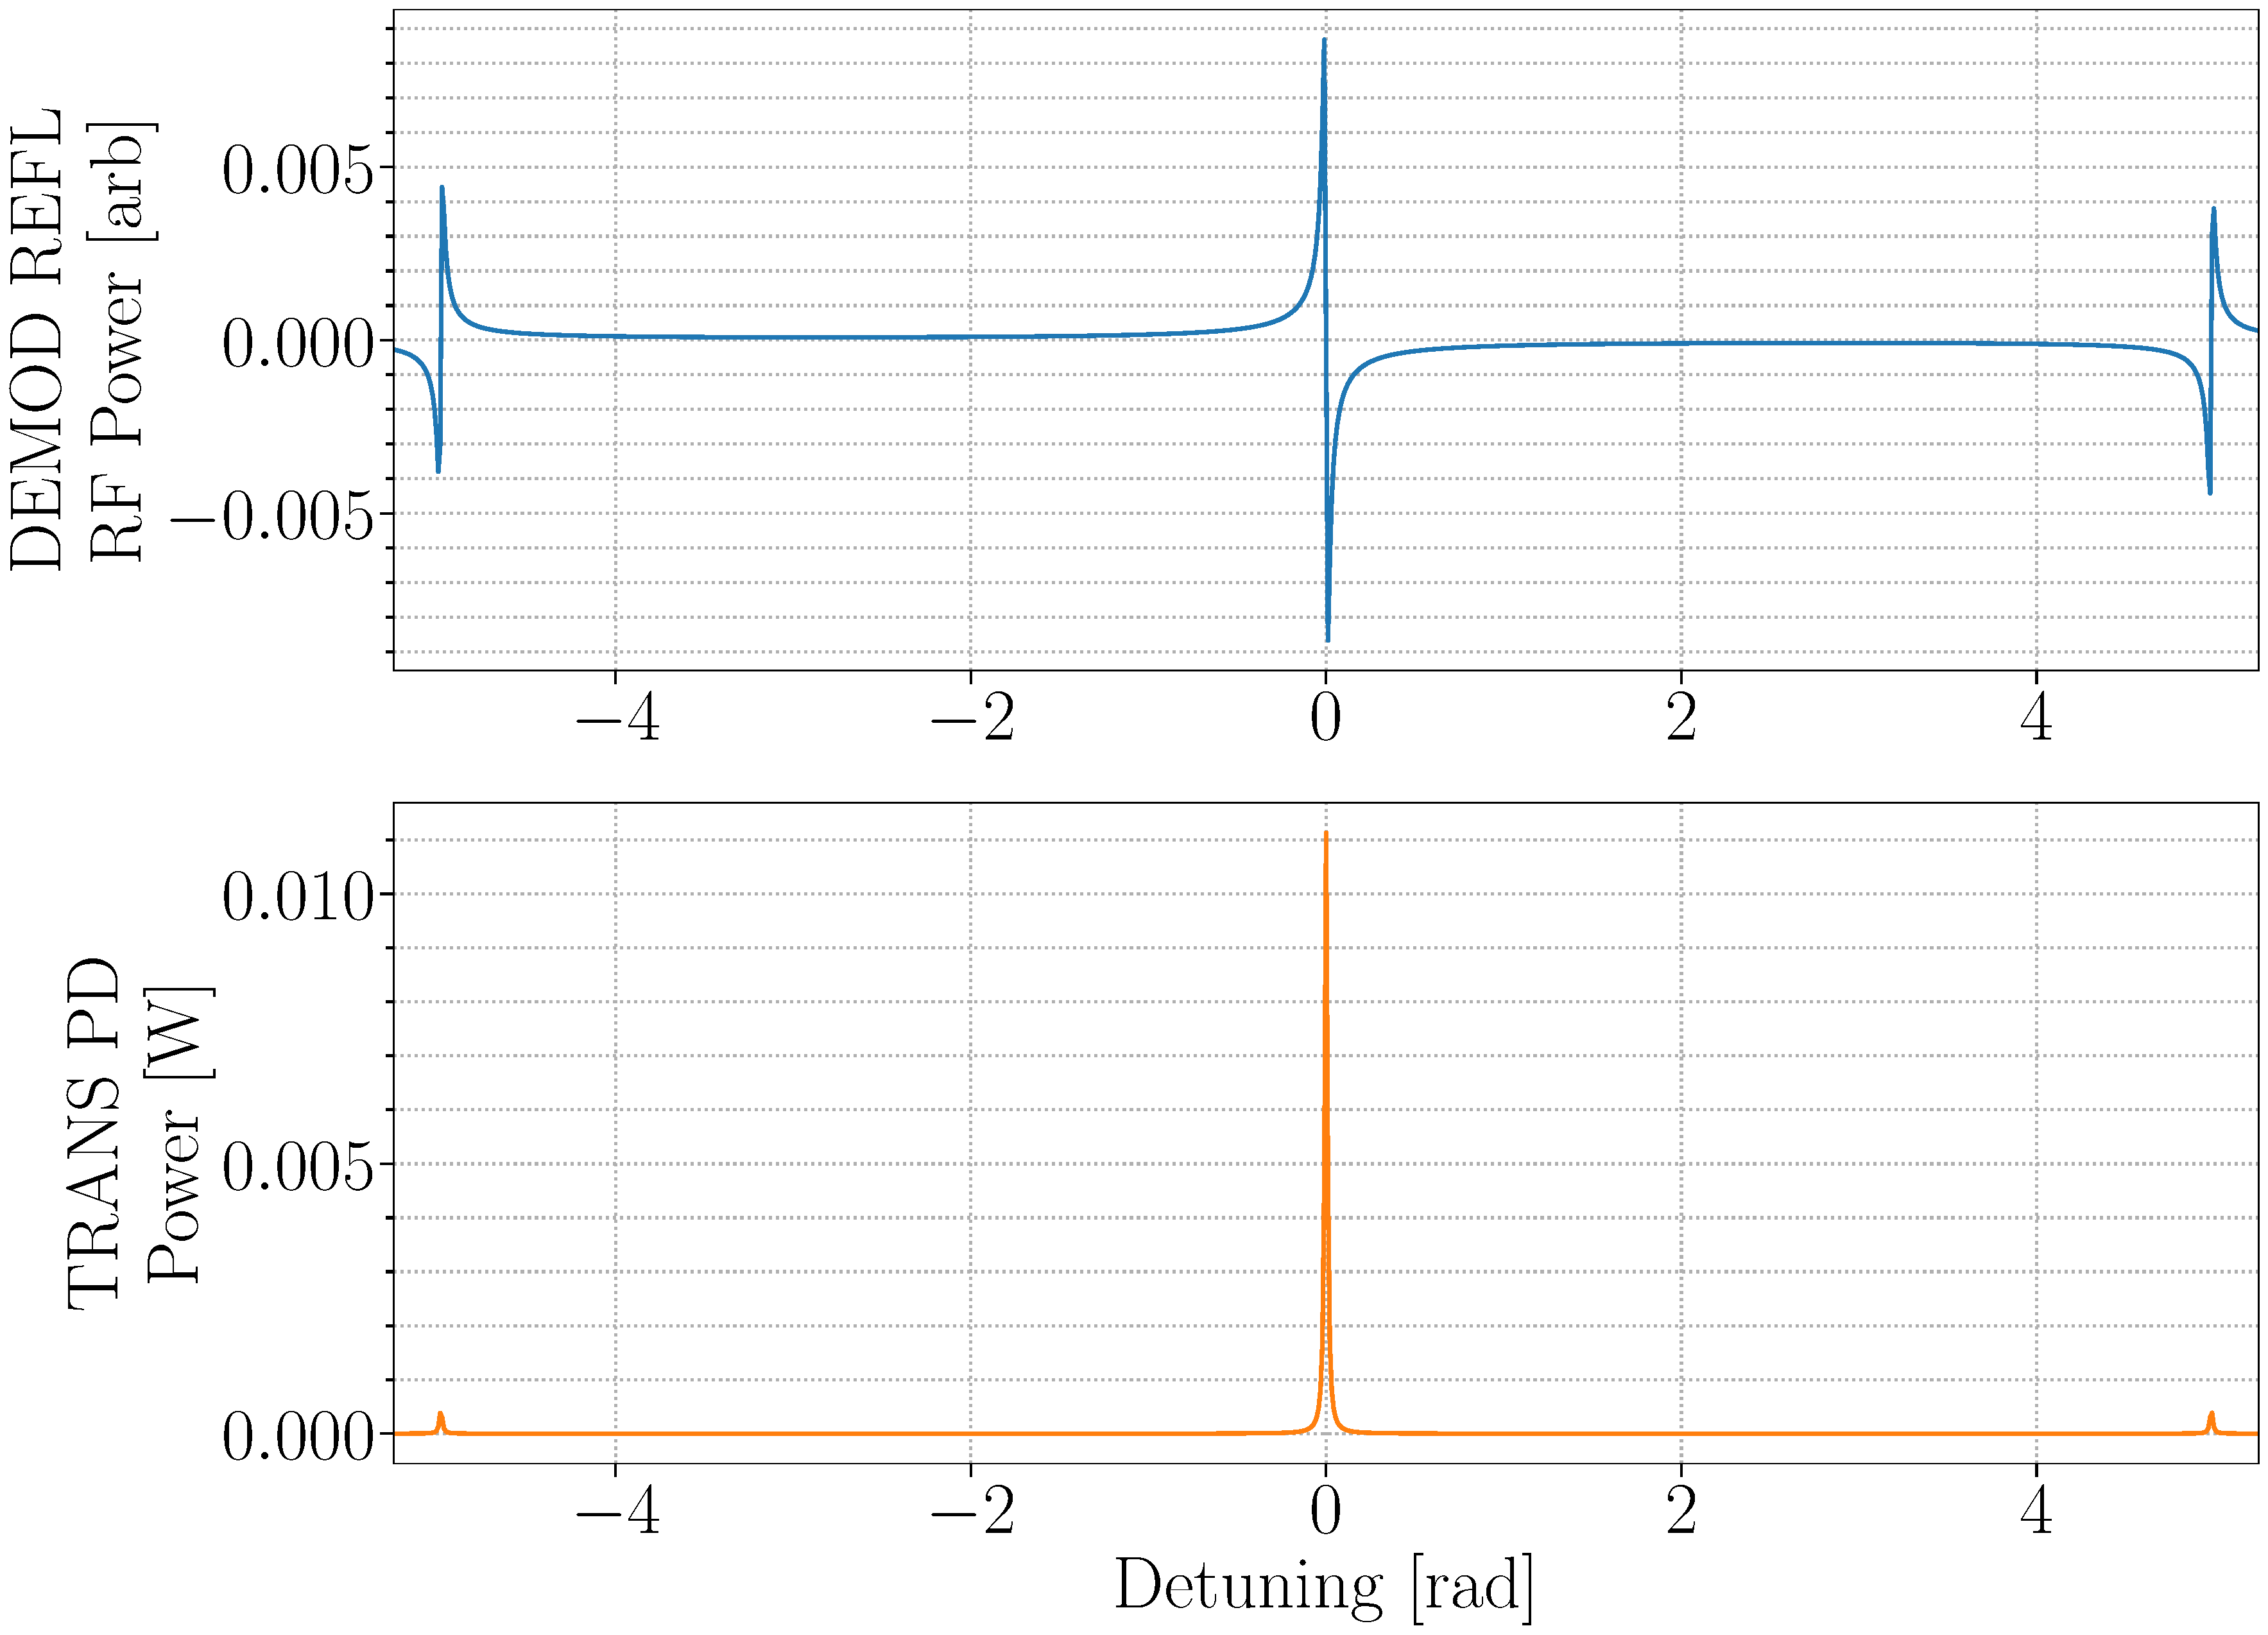
\includegraphics[width=\textwidth]{figs/ALGAAS/pdh_error.pdf}
	\caption{By imposing 25 MHz RF sidebands, a pair of reflected reference fields near carrier resonance are off cavity resonance while beating with the carrier and provide a linear response after demodulating the sideband power. With the introduction of high and low frequency sideband fields, their presence is also detected through the DCPDs and PDH error signal. Their separations from carrier resonance are equal in phase (length, and frequency).}
\label{fig:pdherr}
\end{figure}

With this linearity and sensitivity at cavity resonance, implementation into PID feedback is the next task as any small detuning of the cavity can be registered as a drift from the loop's zero point and fed back to an actuator with an estimated calibration gain factor. When implemented into a low-noise design, this servo can also be used for a high sensitivity lock-in measurement; and with well characterized instrumentation, calibration of the induced differential phase of the light within the stable reference cavity into differential length (or frequency).


\subsection{Servo Parameters}
The actuation portion of the loop begins post the
The quantity we are attempting to measure is a differential length on the order of $3.3 \times 10^{-18}$ [m/(V/m)], motivating a short cavity design as the relative differential length (phase) change scales with the sensitivity \autoref{eq:cavlf}. Considerations of the lab mirror inventory and mode matching critera lead us to two candidate plano-concave (ROC = 0.333m) HR IBS coated sample input couplers; one from CVI Melles-Griot and another from ATFilms. When paired with the plano-plano $\gaas$/$\algaas$  mirror from the Crystalline Mirror Solutions (CMS) division of Thorlabs we create a 0.1665 m long cavity.

%\begin{figure}[H]
%\begin{center}
%\includegraphics[width=.80\textwidth]{ALGAAS/opt_layout_b.pdf}
%\end{center}
%\caption{\textcolor{red}{Final figure still pending} Detailed optical schema of the experiment. Components highlighted in magenta indicate laser back-reflection protection and output power control. All optics highlighted in PURPLE indicate their function as alignment and mode matching for locking to a triangular ALIGO PMC \textbf{Multiple citations (DCC doc / Fabian's experiment / Erik's experiment)}. Optics highlighted in YELLOW indicate function for alignment and mode matching to the experimental cavity utilizing the HR $\gaas$/$\algaas$ coated mirror sample. Beam profiling to the sample cavity is indicated. For the sake of the numerous mounting strategies tried, the longitudinal pockels cell mirror mount is kept general with the pictured mirror between two disk capacitors}
%\label{fig:expoptical_layout}
%\end{figure}
%%FIGURE: Servo diagram
%%CAPTION: A simplified diagram of the servo used. The highlighted regions of the schematic are intended to provide a modular view; highlighting the components required for the PDH servo to operate.}

The implemented servo design uses a light source from a Mephisto 2000 NE Nd:YAG (1064nm) laser with a 25 MHz phase modulation from a New Focus Model 4003 IR resonant phase modulator. As indicated in the figure above, the electronics chain can be decomposed into various filter components: $S(f)$, $A(f)$, and $A_\mathrm{thermal}(f)$

\subsubsection{Sensing S(f)}
Sensing electronics are composed of a single element photodiode mounted to a tranimpedance amplifier PCB that redirects photocurrent to DC and RF outputs. The RF path is constructed so the RF signal is boosted before being passed to a mixer within a frequency stabilization servo (FSS) where it is demodulated by mixing the 25 MHz oscillator phased with variable cable length. Once demodulated, the measured beat signal while sweeping through resonance generates the PDH error signal profile \autoref{fig:pdherr}.

\subsubsection{Actuation A(f)}
The actuation portion of the loop amplifies the FSS output with a single I/O channel of the SVR 350-3 BIP High Voltage Amplifier from Piezomechanik GmbH with a custom pomona box (elog 412) feeding back the output to the input to attentuate ringing. The Mephisto 2220 laser cavity PZT actuator follows immediately after which has a documented linear calibration of 2.0 [MHz] / [V].

\subsubsection{OLG(f)}
Isn't quite $\mathrm{A}(f)*\mathrm{S}(f)$ as stated. Doesn't entirely account for the optical plant.
How the measurement is taken (important to take between installations to account for the changes in the optical plant) (elog 831)

\begin{figure}[H]
\begin{center}
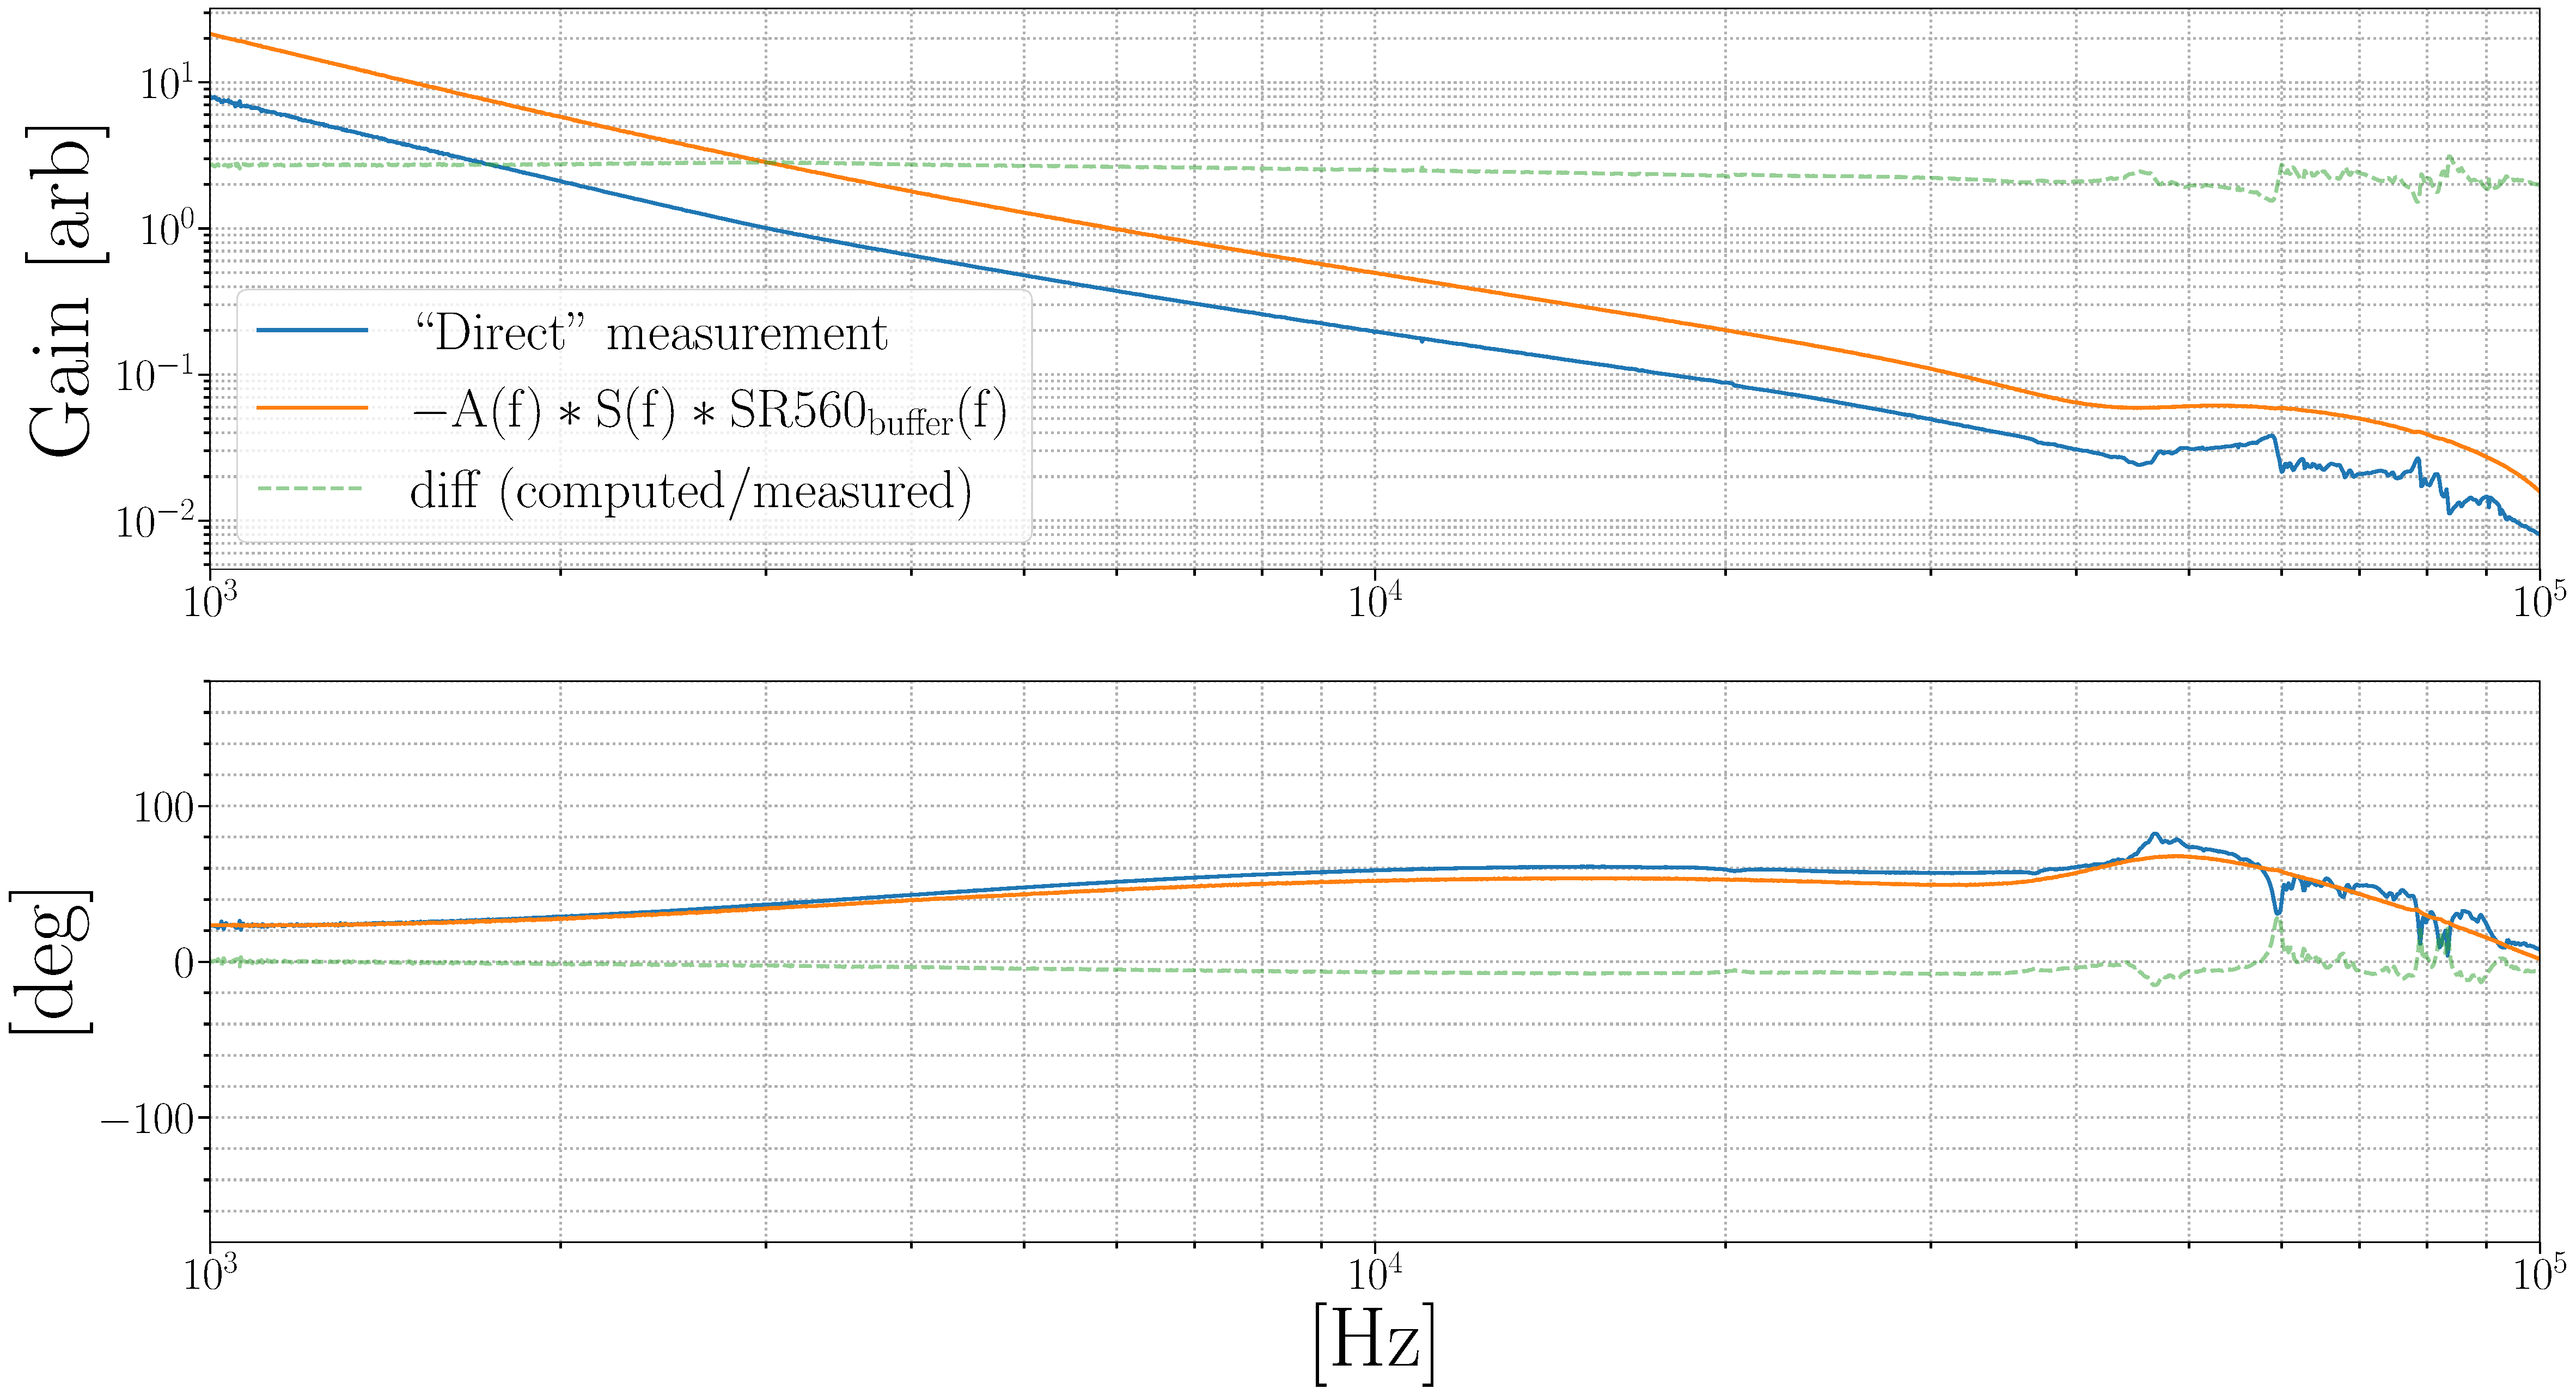
\includegraphics[width=\textwidth]{ALGAAS/olg_compare.pdf}
\end{center}
\caption{Comparison of the open loop gain measurement against the multiplied servo electronics measurements. The maximum gain difference is about a factor of 2.8 which is low passed to a difference of 2.0.}
\label{fig:OLGcompare}
\end{figure}

\subsection{Longitudinal Pockels Cell mirror mount assembly}
Maximizing a controlled and well defined electric field ($|E_z|$) within the coating while requiring a through beam to and through the HR coating lead us to a design very similar to that of a longitudinal pockels cell. The most common assembly in for this study is comprised of two electrodes with a 3mm central aperture which is chosen to be at least 5 times larger than the beam size at the plate locations; to avoid significant beam clipping while maximizing field strength at the coating region of interest. There is also a required separation of at least 1/4" accounting for the thickness of the optical sample. Considering these constraints, modelling the system and computing the estimated field strength screened by the coating is the next step to the construction of the assembly.

\begin{figure}[H]
\begin{center}
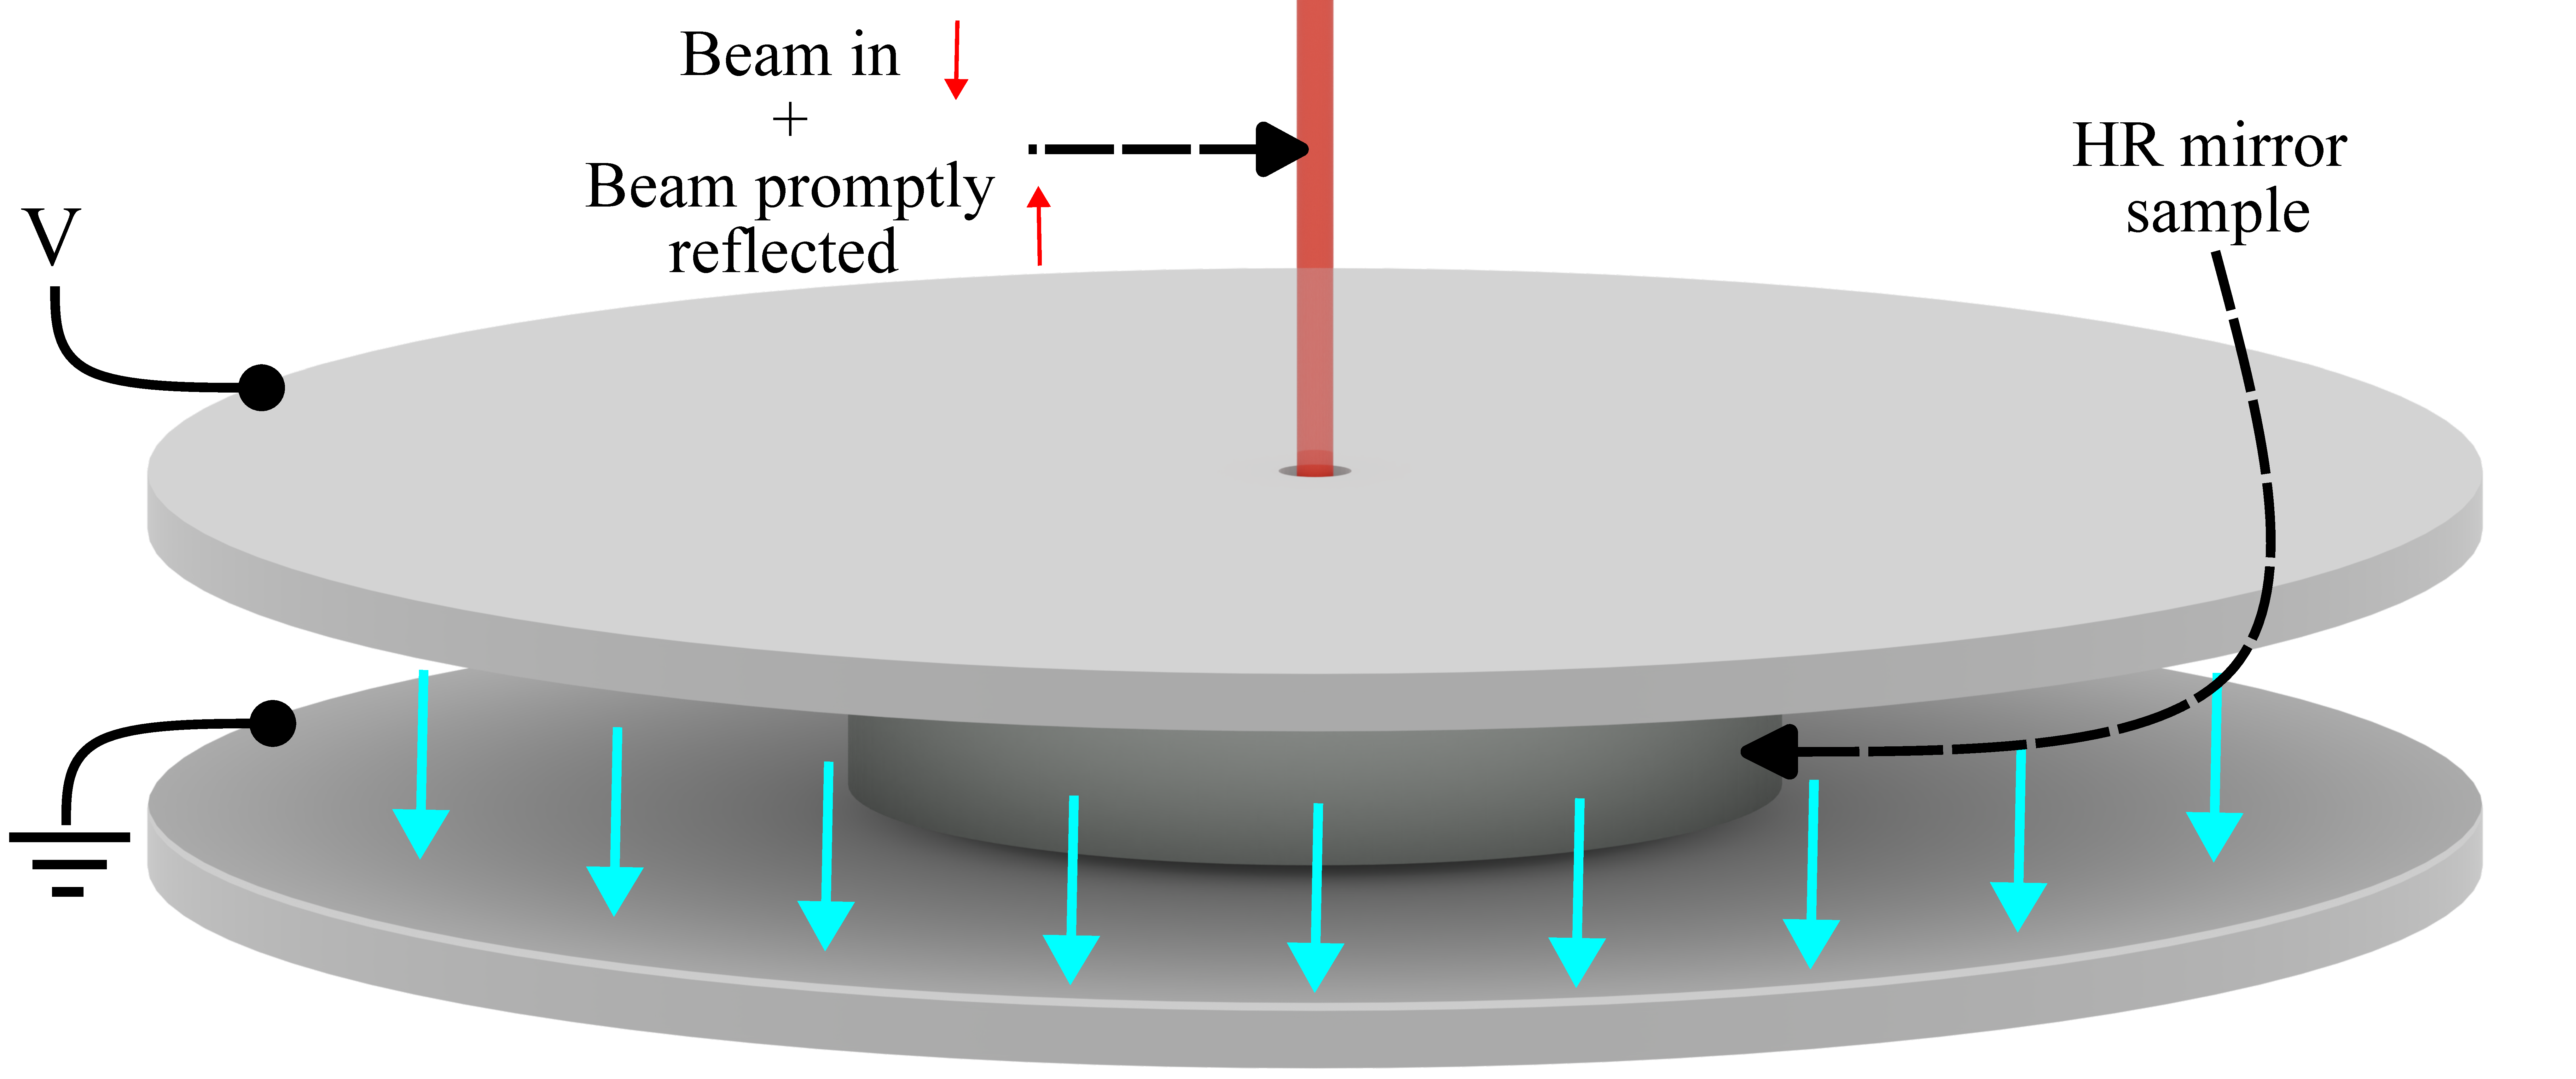
\includegraphics[width=\textwidth]{ALGAAS/longitudinal_pockels_cell_raw_isometric.pdf}
\end{center}
\caption{Concept image of the longitudinal Pockels cell assembly}
\label{fig:pckcellconcept}
\end{figure}

\subsubsection{Modeling}
The field screened by the coating can be computed from Gauss' Law:
\begin{equation}
\nabla \cdot D = \rho_\mathrm{free}
\end{equation}

\noindent There is no free charge within the region of interest ($\rho_\mathrm{free}=0$), though the optic sample fused silica substrate with the AlGaAs coating imposes dielectric material between the plates. Boundary conditions are expressed in terms of the differential plate potential $V$, so it is natural to first solve the potential ($V$) for all relevant system coordinate points.  

\begin{equation}\label{eq:cyllap}
\nabla^2 V = 0
\end{equation}

\paragraph*{Boundary Conditions}

\begin{figure}[H]
  \centering
  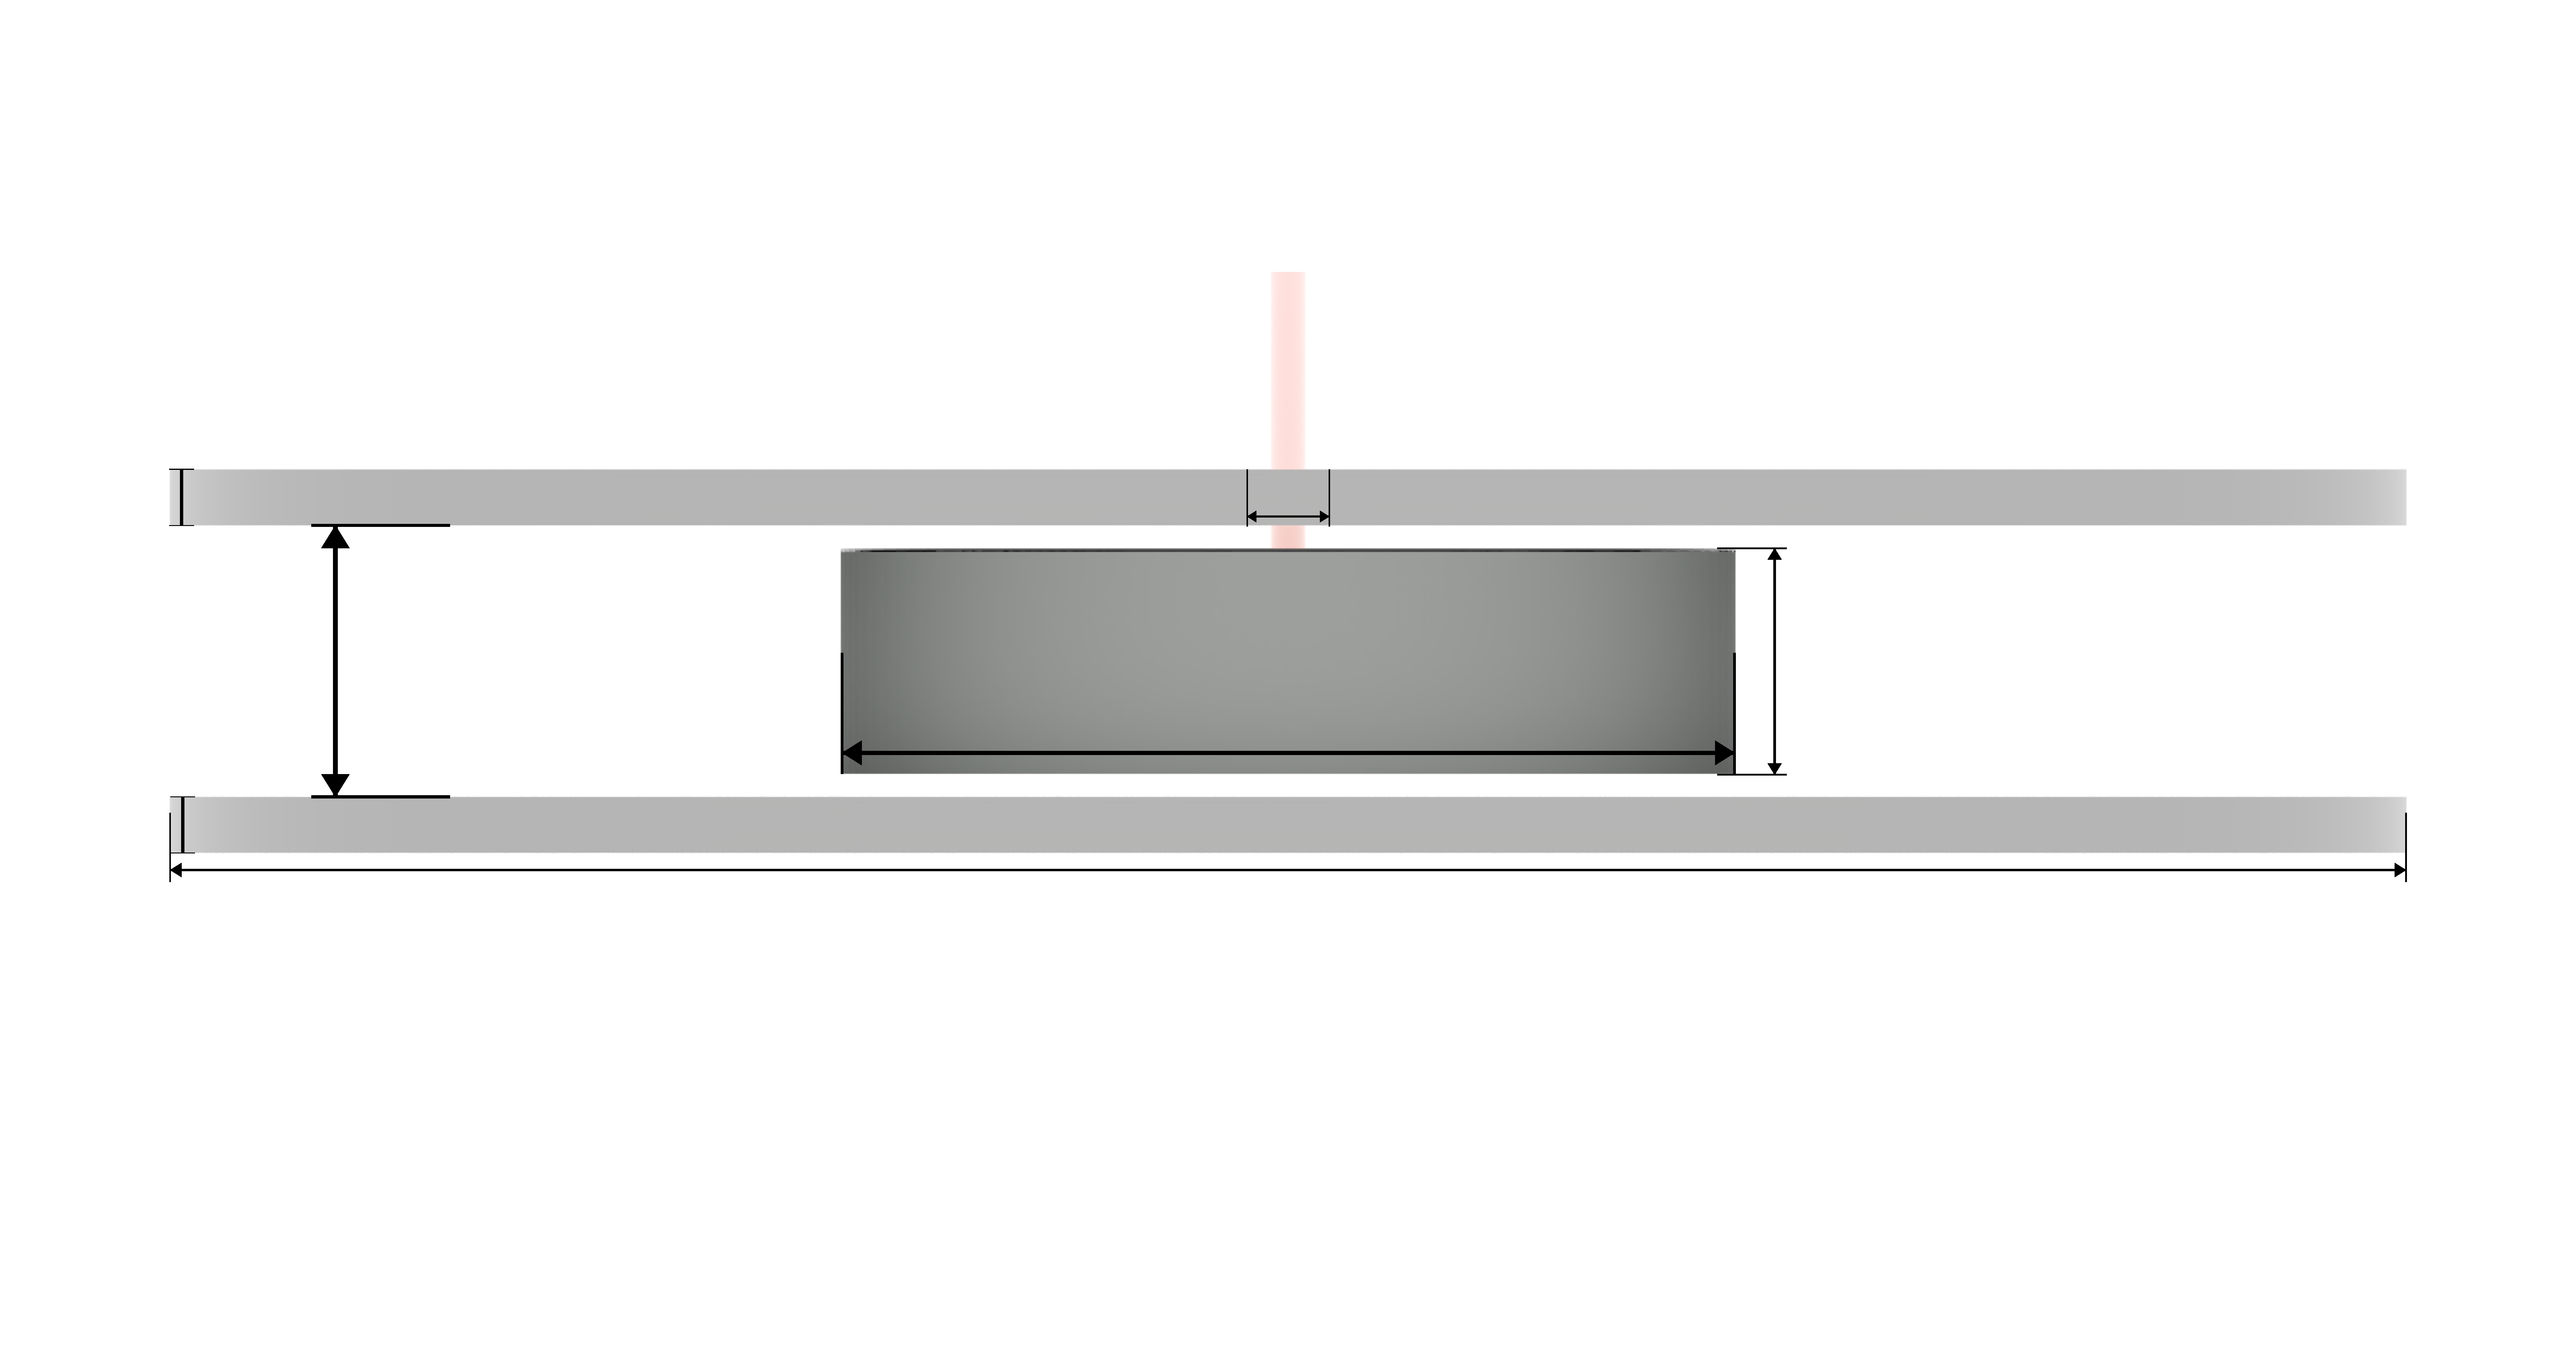
\includegraphics[width=\textwidth]{ALGAAS/longitudinal_pockels_cell_bc.pdf}
\caption{Side view of the longitudinal pockels cell mount. The figure is annotated with relevant parameters to build the numerical model: the finite thicknesses of the electrode plates ($t_{el}$) , radius of the aperture at the center of the disk ($r_{ap}$), radius of the disk ($r_d$),thickness of the optic ($t_{opt}$),and radius of the optic substrate ($r_{opt}$)}
  %%Use relevant cross sectional figure to establish coordinates for $\gaas$/$\algaas$, as well as the fused silica substrate so the computation is transparent.} Cross sectional diagram indicating relevant axes and boundary conditions utilized in the numerical computation
  \label{fig:laplacecoords}
\end{figure}


\subparagraph*{Substrate:}
$ -t_{opt} \; \textless \; z \; \textless \;\mathrm{t}_{opt} $ and $\mathrm{r} \; \textless \;\mathrm{r}_{opt}$
\subparagraph*{Coating}
$\mathrm{t}_{opt} \; \textless \; z \; \textless \;\mathrm{t}_{opt} +\mathrm{t}_{coat} $ and $\mathrm{r} \; \textless \;\mathrm{r}_{opt} $

\subparagraph*{Driven Electrode (V):}
$\mathrm{t}_{cap} \; \textless \; z \; \textless \;\mathrm{t}_{cap} + 2t_{el} $ and $\mathrm{r}_{ap} \; \textless \;\mathrm{r} \; \textless \;\mathrm{r}_{d} $

\subparagraph*{Grounded Electrode (GND):}
$ -t_{cap} -2t_{el} \; \textless \; z \; \textless \; -t_{cap} $ and $\mathrm{r}_{ap} \; \textless \;\mathrm{r} \; \textless \;\mathrm{r}_{d} $

\paragraph*{Numerical Recipe (Finite Differencing)}

We exploit the chosen optic / disk symmetry about the polar angle ($\partial V / \partial \theta = 0$) and compute for the longitudinal ($z$) and radial ($r$) coordinates with the use of the appropriate Laplacian:

\begin{equation} 
\bigg[\frac{1}{r}\frac{\partial}{\partial r} \bigg( r \frac{\partial}{\partial r}\bigg) + \frac{\partial^2}{\partial z^2} \bigg](\varepsilon V) = 0
\end{equation}

Where $\varepsilon$ is the dielectric

Observing equation \autoref{eq:cyllap} we parse the non-zero expression into it's individual parts:

\begin{equation} \label{eq:cyllap_xpand}
    \bigg[\underbrace{\frac{\partial^2}{\partial z^2}}_\text{(c)} + \underbrace{\frac{\partial^2}{\partial r^2}}_\text{(b)}  + \underbrace{\frac{1}{r} \frac{\partial}{\partial r}}_\text{(a)}\bigg] (\varepsilon V) = 0
\end{equation}

\subparagraph*{Term (a)}

Starting with the first derivative, we use the central difference approximation:

\begin{equation}
    \frac{\partial}{\partial r} \rightarrow \frac{f(r + h, z) - f(r - h, z )}{2h} \rightarrow \bigg[-\frac{1}{2} \quad  0  \quad \frac{1}{2} \bigg]
\end{equation}

\subparagraph*{Term (b)}

Second derivative approximation, we use the standard 2d laplace stencil

\begin{equation}
    \frac{\partial}{\partial r^2} \rightarrow \frac{f(r+h, z) - 2 f(r, z) + f(r-h, z)}{h^2} \rightarrow \big[ 1 \quad -2 \quad 1 \big]
\end{equation}

\subparagraph*{Term (c)}
Equivalent to the second derivative approximation used above:

\begin{equation}
    \frac{\partial}{\partial z^2} \rightarrow  \frac{f(r, z+h) - 2 f(r, z) + f(r, z-h)}{h^2} \rightarrow \big[ 1\quad -2 \quad 1 \big]
\end{equation}

To build the stencil terms at the boundaries, we look at the specialized finite difference condition @ $ r = 0 $, with the symmetry about $r=0$ allowing the application of a ghost point V(-h,z) as V(h,z) :

\begin{equation}\label{eq:first_deriv_V}
	\frac{\partial V}{\partial r} = 0 \rightarrow V(h, z) = V(-h,z)
\end{equation}

\begin{equation}\label{eq:second_deriv_V}
	\frac{\partial^2 V}{\partial r^2} = \frac{2}{h}\bigg(\frac{V(h,z) -  V(0, z) }{h}\bigg) 
\end{equation}

\autoref{eq:first_deriv_V} alone does not define V(0,z), to establish the form of this point, we proceed to (Taylor) expand the function about it:

\begin{equation}\label{eq:taylor_V}
 V \approx V_0  + C_1 r +  C_2 r^{2} + \mathcal{O}(r^4) 
\end{equation}

Symmetry about the origin imposes an even function of $V$:  
$$ \frac{\partial V}{\partial r} \approx C_1 +  2 C_2 r  + \mathcal{O}(r^3) $$

\begin{equation}\label{eq:taylor_terma}
	\frac{1}{r} \frac{\partial V}{\partial r} \approx  2 C_2  + \mathcal{O}(r^2)
\end{equation}

Where $C_1 = 0$ to avoid a singular point.

\begin{equation}\label{eq:taylor_termb}
	\frac{\partial^2 V}{\partial r^2} \approx 2 C_2 + \mathcal{O}(r^2) 
\end{equation}

Substituting \autoref{eq:taylor_terma} and \autoref{eq:taylor_termb} back into equation \autoref{eq:cyllap_xpand} :
\begin{equation}
    \nabla^2 (\varepsilon V)= \frac{\partial^2}{\partial z^2} + 4 C_2 
\end{equation}

The radial portion of the operator $\nabla^2 V$ given \autoref{eq:taylor_V} and \autoref{eq:second_deriv_V}:

\begin{equation}
\bigg(\frac{r_0}{h} - \frac{2}{h^2} \bigg) C_1 + \bigg(\frac{r_h}{h} + \frac{2}{h^2} \bigg) C_2 h^2 = 4 C_2
\end{equation}

Where again, we found $C_1 = 0$:

$$
(r_h * h + 2) C_2 = 4 C_2
$$

\begin{equation}
    \begin{aligned}
	r_h = 2 / h  \; , \\
	r_0 = -2 / h
    \end{aligned}
\end{equation}

Now meshgrid coordinates are set:

%% Meshgrid indexing

\[
z_\mathrm{indexing} \rightarrow 
\begin{bmatrix*}[c] \,
z_0 & z_0 & z_0 & z_0 & z_0 & z_0 & z_0 & z_0 & z_0 & \cdots & \cdots\\
z_1 & z_1 & z_1 & z_1 & z_1 & z_1 & z_1 & z_1 & z_1 & \cdots & \cdots\\
z_2 & z_2 & z_2 & z_2 & z_2 & z_2 & z_2 & z_2 & z_2 & \cdots & \cdots\\
z_3 & z_3 & z_3 & z_3 & z_3 & z_3 & z_3 & z_3 & z_3 & \cdots & \cdots\\
z_4 & z_4 & z_4 & z_4 & z_4 & z_4 & z_4 & z_4 & z_4 & \cdots & \cdots\\
z_5 & z_5 & z_5 & z_5 & z_5 & z_5 & z_5 & z_5 & z_5 & \cdots & \cdots\\
z_6 & z_6 & z_6 & z_6 & z_6 & z_6 & z_6 & z_6 & z_6 & \cdots & \cdots\\
z_7 & z_7 & z_7 & z_7 & z_7 & z_7 & z_7 & z_7 & z_7 & \cdots & \cdots\\
z_8 & z_8 & z_8 & z_8 & z_8 & z_8 & z_8 & z_8 & z_8 & \cdots & \cdots\\
\vdots & \vdots & \vdots & \vdots & \vdots & \vdots & \vdots & \vdots & \vdots & \ddots & \cdots\\
z_n & z_n & z_n & z_n & z_n & z_n & z_n & z_n & z_n & \cdots & \ddots\\
\end{bmatrix*}
\]

\[
\rho_\mathrm{indexing} \rightarrow 
\begin{bmatrix*}[c] \,
\rho_0 & \rho_1 & \rho_2 & \rho_3 & \rho_4 & \rho_5 & \rho_6 & \rho_7 & \rho_8 & \cdots & \rho_n\\
\rho_0 & \rho_1 & \rho_2 & \rho_3 & \rho_4 & \rho_5 & \rho_6 & \rho_7 & \rho_8 & \cdots & \rho_n\\
\rho_0 & \rho_1 & \rho_2 & \rho_3 & \rho_4 & \rho_5 & \rho_6 & \rho_7 & \rho_8 & \cdots & \rho_n\\
\rho_0 & \rho_1 & \rho_2 & \rho_3 & \rho_4 & \rho_5 & \rho_6 & \rho_7 & \rho_8 & \cdots & \rho_n\\
\rho_0 & \rho_1 & \rho_2 & \rho_3 & \rho_4 & \rho_5 & \rho_6 & \rho_7 & \rho_8 & \cdots & \rho_n\\
\rho_0 & \rho_1 & \rho_2 & \rho_3 & \rho_4 & \rho_5 & \rho_6 & \rho_7 & \rho_8 & \cdots & \rho_n\\
\rho_0 & \rho_1 & \rho_2 & \rho_3 & \rho_4 & \rho_5 & \rho_6 & \rho_7 & \rho_8 & \cdots & \rho_n\\
\rho_0 & \rho_1 & \rho_2 & \rho_3 & \rho_4 & \rho_5 & \rho_6 & \rho_7 & \rho_8 & \cdots & \rho_n\\
\rho_0 & \rho_1 & \rho_2 & \rho_3 & \rho_4 & \rho_5 & \rho_6 & \rho_7 & \rho_8 & \cdots & \rho_n\\
\rho_0 & \rho_1 & \rho_2 & \rho_3 & \rho_4 & \rho_5 & \rho_6 & \rho_7 & \rho_8 & \cdots & \rho_n\\
\vdots & \vdots & \vdots & \vdots & \vdots & \vdots & \vdots & \vdots & \vdots & \ddots & \vdots \\
\vdots & \vdots & \vdots & \vdots & \vdots & \vdots & \vdots & \vdots & \vdots & \vdots & \ddots \\
\end{bmatrix*}
\]


\newpage

Parallel computation of the potential over the entire meshgrid is done by vectorizing the potential:

\[ 
 \begin{aligned}
    V &= \begin{bmatrix}
           V(\rho_0, z_0) \\
           V(\rho_1, z_0) \\
           \vdots \\
	   V(\rho_n, z_0) \\
	   ---------- \\
	   V(\rho_0, z_1) \\
           V(\rho_1, z_1) \\
           \vdots \\
	   V(\rho_n, z_1) \\
	   ---------- \\
	   \vdots \\
	   ---------- \\
	   V(\rho_0, z_{n-1}) \\
           V(\rho_1, z_{n-1}) \\
           \vdots \\
           V(\rho_n, z_{n-1}) \\
           ---------- \\
           V(\rho_0, z_n) \\
	   V(\rho_1, z_n) \\
	   \vdots \\
	   V(\rho_n, z_n) 
         \end{bmatrix}
  \end{aligned}
\]

\newpage
\noindent Inspired by the second-order elliptic equation, operators are modified to incorporate the aforementioned boundary conditions~\cite{Press:2007}:

\[ 
\mathcal{L}_{cyl} = 
\begin{bmatrix} \,
O_{n} & O_{n} & O_{n} & O_{n} & O_{n} & \cdots & \cdots & \cdots & \cdots & \cdots & O_{n}\\
\mathcal{I}_{n} & \mathcal{K}_{n}^{*} & \mathcal{I}_{n} & O_{n} & O_{n} & O_{n} & O_{n} & O_{n} & O_{n} & O_{n} & \vdots\\
O_{n} & \mathcal{I}_{n} & \mathcal{K}_{n}^{*} & \mathcal{I}_{n} & O_{n} & O_{n} & O_{n} & O_{n} & O_{n} & O_{n} & \vdots\\
O_{n} & O_{n}  & \mathcal{I}_{n} & \mathcal{K}_{n}^{*} & \mathcal{I}_{n} & O_{n} & O_{n} & O_{n} & O_{n} & O_{n} & \vdots\\
\vdots & O_{n}  & O_{n}  & \ddots & \ddots & \ddots & O_{n} & O_{n} & O_{n} & O_{n}  & \vdots \\
\vdots & O_{n}  & O_{n}  & O_{n}  & \ddots & \ddots & \ddots & O_{n} & O_{n} & O_{n} & \vdots \\
\vdots & O_{n}  & O_{n}  & O_{n} & O_{n} & \ddots & \ddots & \ddots & O_{n} & O_{n}  & \vdots \\
\vdots & O_{n}  & O_{n}  & O_{n} & O_{n} & O_{n} & \mathcal{I}_{n} & \mathcal{K}_{n}^{*} & \mathcal{I}_{n} & O_{n}  & \vdots\\
\vdots & O_{n}  & O_{n}  & O_{n} & O_{n} & O_{n} & O_{n} & \mathcal{I}_{n} & \mathcal{K}_{n}^{*}  & \mathcal{I}_{n} & O_{n}\\
\vdots & O_{n} & O_{n} & O_{n} & O_{n} & O_{n} & O_{n} & O_{n} & \mathcal{I}_{n} & \mathcal{K}_{n}^{*} & \mathcal{I}_{n}\\
O_{n}      & \cdots & \cdots & \cdots & \cdots & \cdots & O_{n} & O_{n} & O_{n} & O_{n} & {O}_{n}
\end{bmatrix} 
\]

\[
    \mathcal{K}_n^{(1)} = 
\frac{1}{h}
\begin{bmatrix*}[c] \,
0 & 0 & 0 & 0& 0 & \cdots & \cdots & \cdots & \cdots & \cdots & 0 \\
\frac{1}{2} & 0 & \frac{1}{2} & 0 & 0 & 0 & 0 & 0 & 0 & 0 & \vdots \\
0 & \frac{1}{4} & 0 & \frac{1}{4} & 0 & 0 & 0 & 0 & 0 & 0 & \vdots \\
0 & 0 & \frac{1}{6} & 0 & \frac{1}{6} & 0 & 0 & 0 & 0 & 0 & \vdots \\
\vdots & 0  & 0  & \ddots & \ddots & \ddots & 0 & 0 & 0 & 0  & \vdots \\
\vdots & 0  & 0  & 0  & \ddots & \ddots & \ddots & 0 & 0 & 0 & \vdots \\
\vdots & 0  & 0  & 0 & 0 & \ddots & \ddots & \ddots & 0 & 0  & \vdots \\
\vdots & 0  & 0  & 0 & 0 & 0 & \ddots & 0 & \frac{1}{2^{(n-4)}} & 0  & \vdots\\
\vdots & 0  & 0  & 0 & 0 & 0 & 0 & \frac{1}{2^{(n-3)}} & 0  & \frac{1}{2^{(n-3)}} & 0\\
\vdots & 0 & 0 & 0 & 0 & 0 & 0 & 0 & \frac{1}{2^{(n-2)}} & 0 & \frac{1}{2^{(n-2)}}\\
0      & \cdots & \cdots & \cdots & \cdots & \cdots & 0 & 0 & 0 & 0 & 0 
\end{bmatrix*}
\]

\[
    \mathcal{K}_n^{(2)}  = 
\frac{1}{h^2}
\begin{bmatrix} \,
-6 & 4 & 0 & 0& 0 & \cdots & \cdots & \cdots & \cdots & \cdots & 0 \\
1 & -4 & 1 & 0 & 0 & 0 & 0 & 0 & 0 & 0 & \vdots \\
0 & 1 & -4 & 1 & 0 & 0 & 0 & 0 & 0 & 0 & \vdots \\
0 & 0 & \ddots & \ddots & \ddots & 0 & 0 & 0 & 0 & 0 & 0 \\
\vdots & 0  & 0  & \ddots & \ddots & \ddots & 0 & 0 & 0 & 0  & \vdots \\
\vdots & 0  & 0  & 0  & \ddots & \ddots & \ddots & 0 & 0 & 0 & \vdots \\
\vdots & 0  & 0  & 0 & 0 & \ddots & \ddots & \ddots & 0 & 0  & \vdots \\
\vdots & 0  & 0  & 0 & 0 & 0 & \ddots & -4 & 1 & 0  & \vdots\\
\vdots & 0  & 0  & 0 & 0 & 0 & 0 & 1 & -4  & 1 & 0\\
\vdots & 0 & 0 & 0 & 0 & 0 & 0 & 0 & 1 & -4 & 1\\
0      & \cdots & \cdots & \cdots & \cdots & \cdots & 0 & 0 & 0 & 0 & 0 
\end{bmatrix}
\]

\[
	\mathcal{K}_n^{*} = \mathcal{K}_n^{(1)} + \mathcal{K}_n^{(2)} 
\]

\[
    \mathcal{I}_n = \frac{1}{h^2} \bigg( \mathrm{eye}(n) - (\mathrm{zeros}(n)[n,n] + 1) \bigg)
\]

\[ 
	O_{n} = \mathrm{zeros}(n)
\]	
Where the above matrix is a tri-diagonal block sparse matrix with square embedded diagonal identity ($\mathcal{I}_n$) matrices with n non-zero diagonal elements, and sparse tridiagonal kernel ($\mathcal{K}_n$) matrices. $O_n$ presents zero matrices with $n\times n$ sharing the dimensions of $\mathcal{K}_n$ and $\mathcal{I}_n$. \footnote{Not completely clear to the author at first, the motivation behind the structural choice of sparse block diagonals is a symptom of continuously vectorizing the computation. Some standard computing libraries may be proactive about this vectorization and apply it when recognized in for-loops. Even so, the explicit structuring of the boundary conditions listed here is intended to inform of the reasoning behind the modified numerical recipe to establish a compartmentalization between the scientific motivation alongside computing tools and methods.}

\newpage

\noindent Computing Potential:

\begin{equation}
    V_{n + 1} = (\mathcal{I}_{N^2}  + \mathcal{L}_{cyl}) V_{n}
\end{equation}

\begin{figure}[H]
  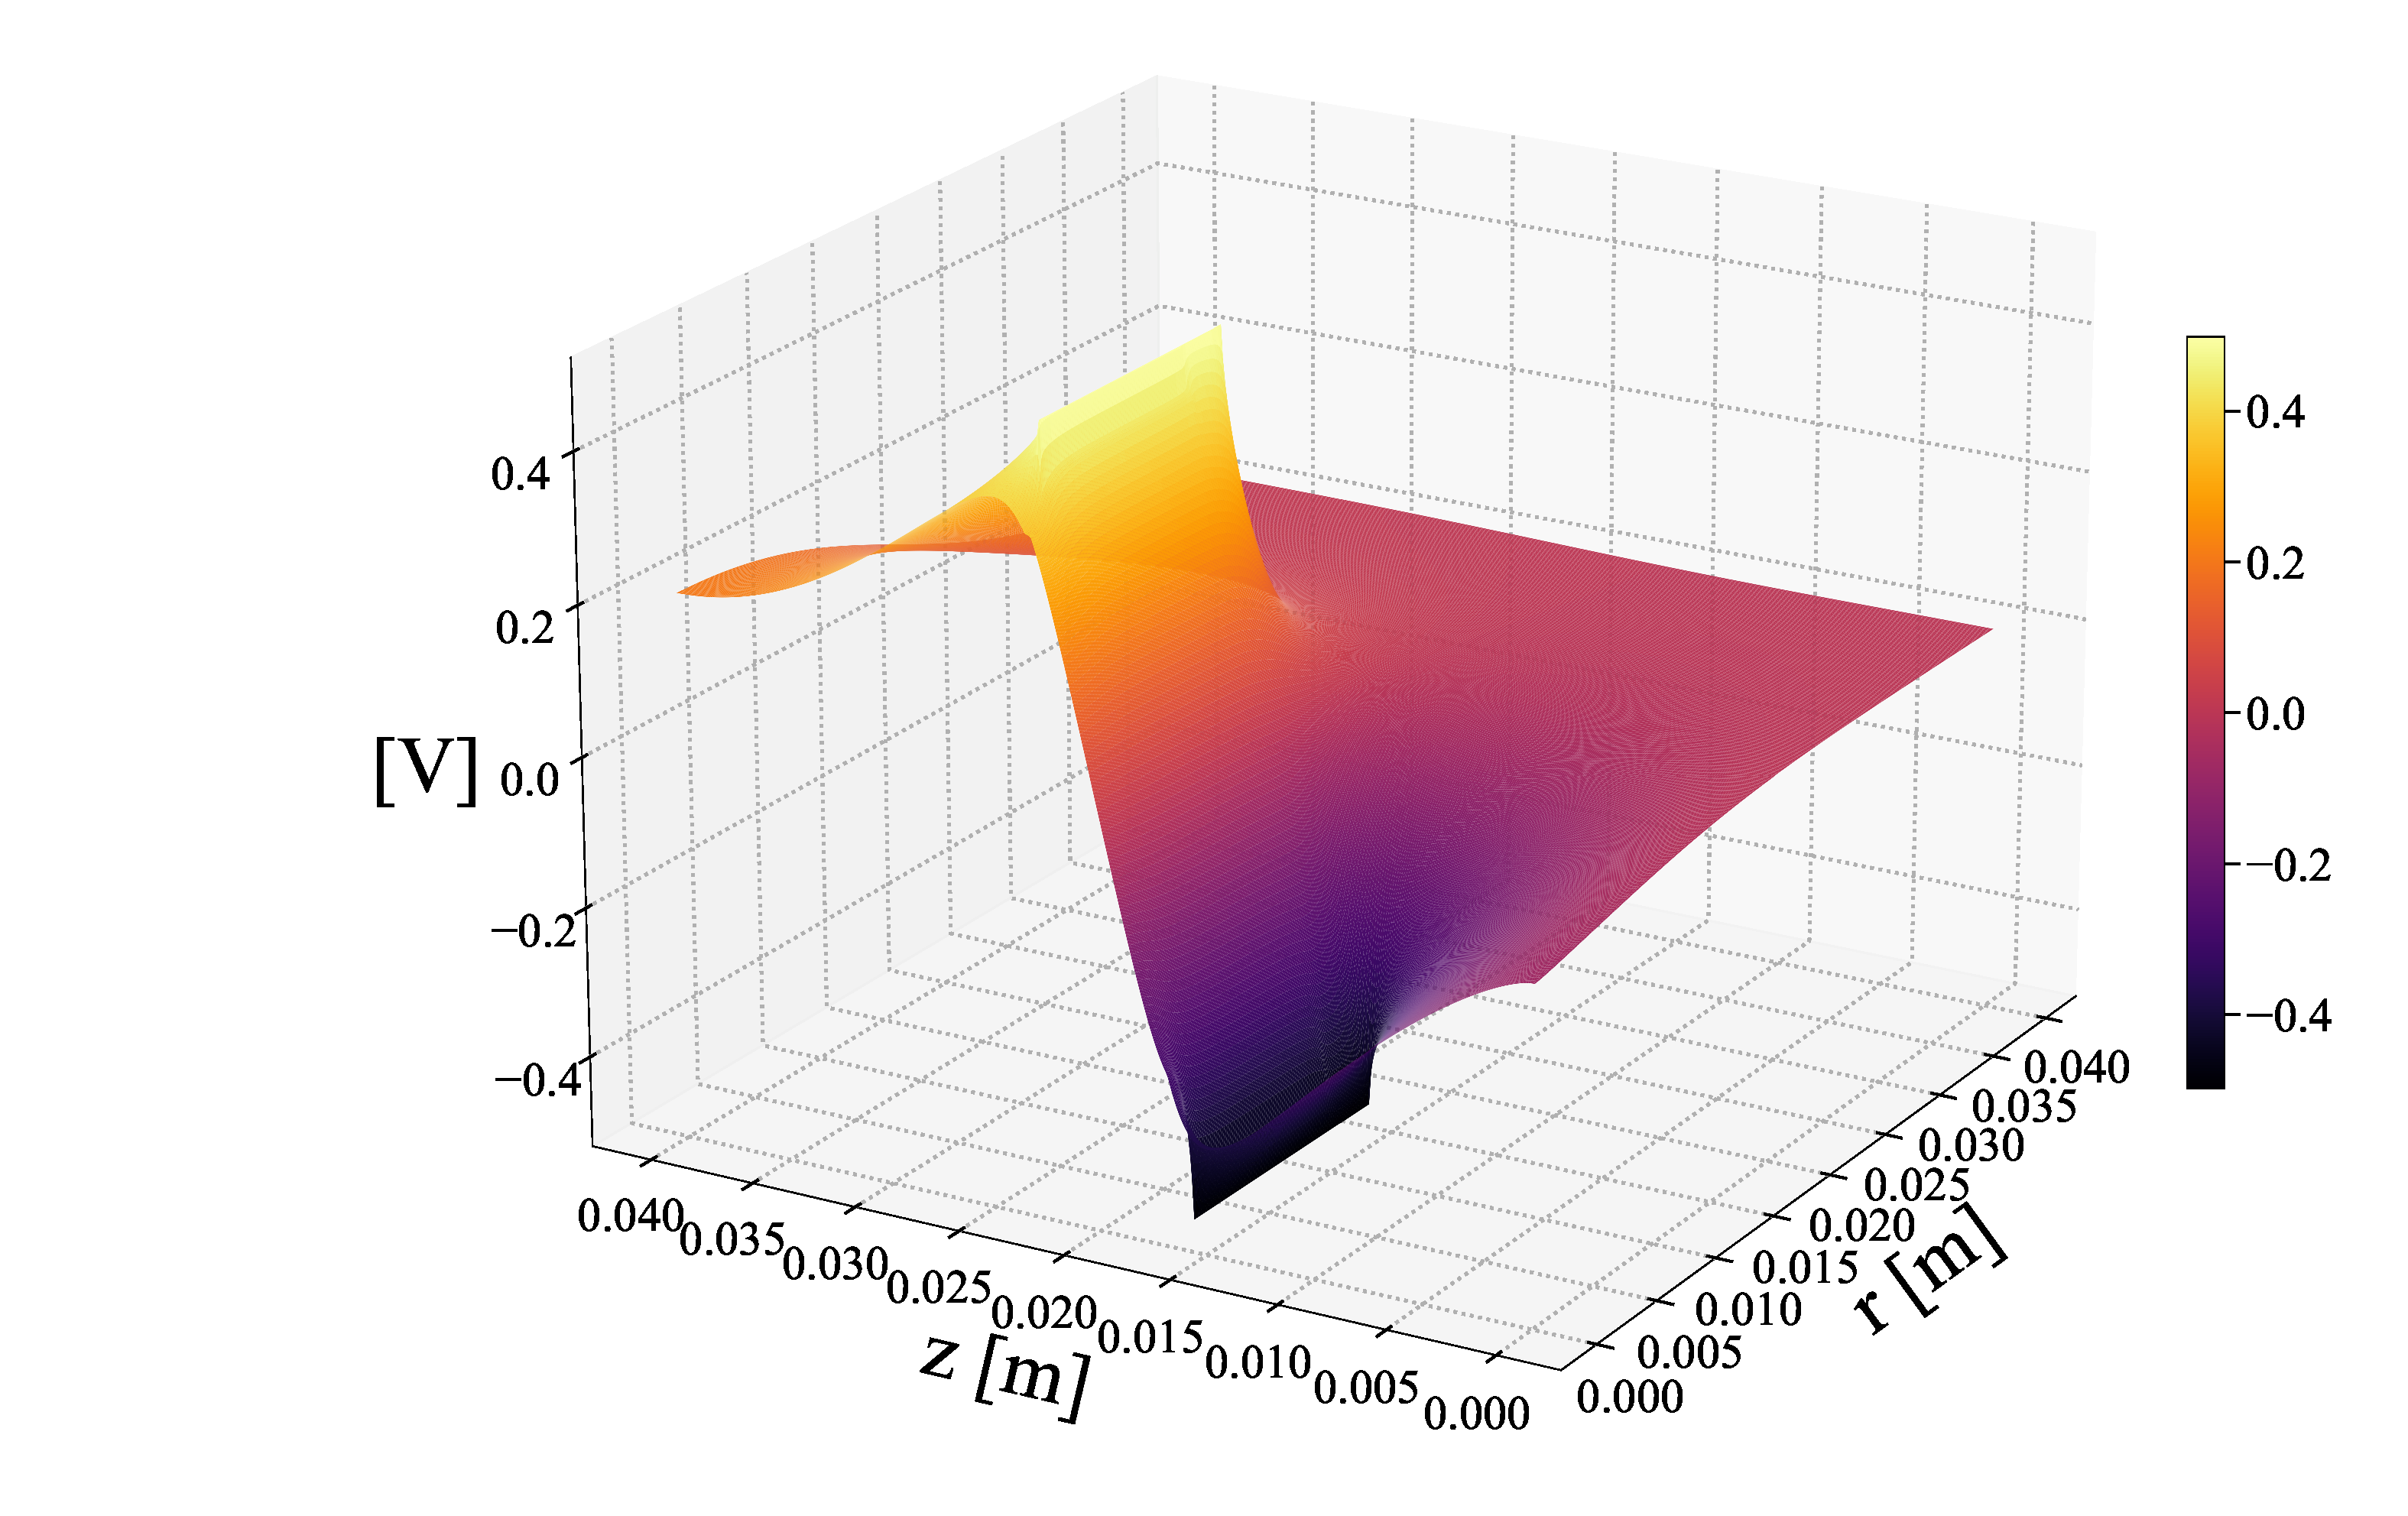
\includegraphics[width=\textwidth]{ALGAAS/assembly4_sim.pdf}
  \caption{Numerically computed potential map estimate ($V(z,r)$ in cylindrical coordinates)}
  \label{fig:poissoncalcoutput}
\end{figure}

The computed $E_z$ screened by the coating at $r = 0$ for $V = 1$ is estimated to be 13.3 $[\mathrm{V}/\mathrm{m}]$ and will be included in the calibration as a pockels cell conversion efficiency of 13.3 $[(\mathrm{V} / \mathrm{m}) / \mathrm{V}]$  

\begin{figure}[H]
    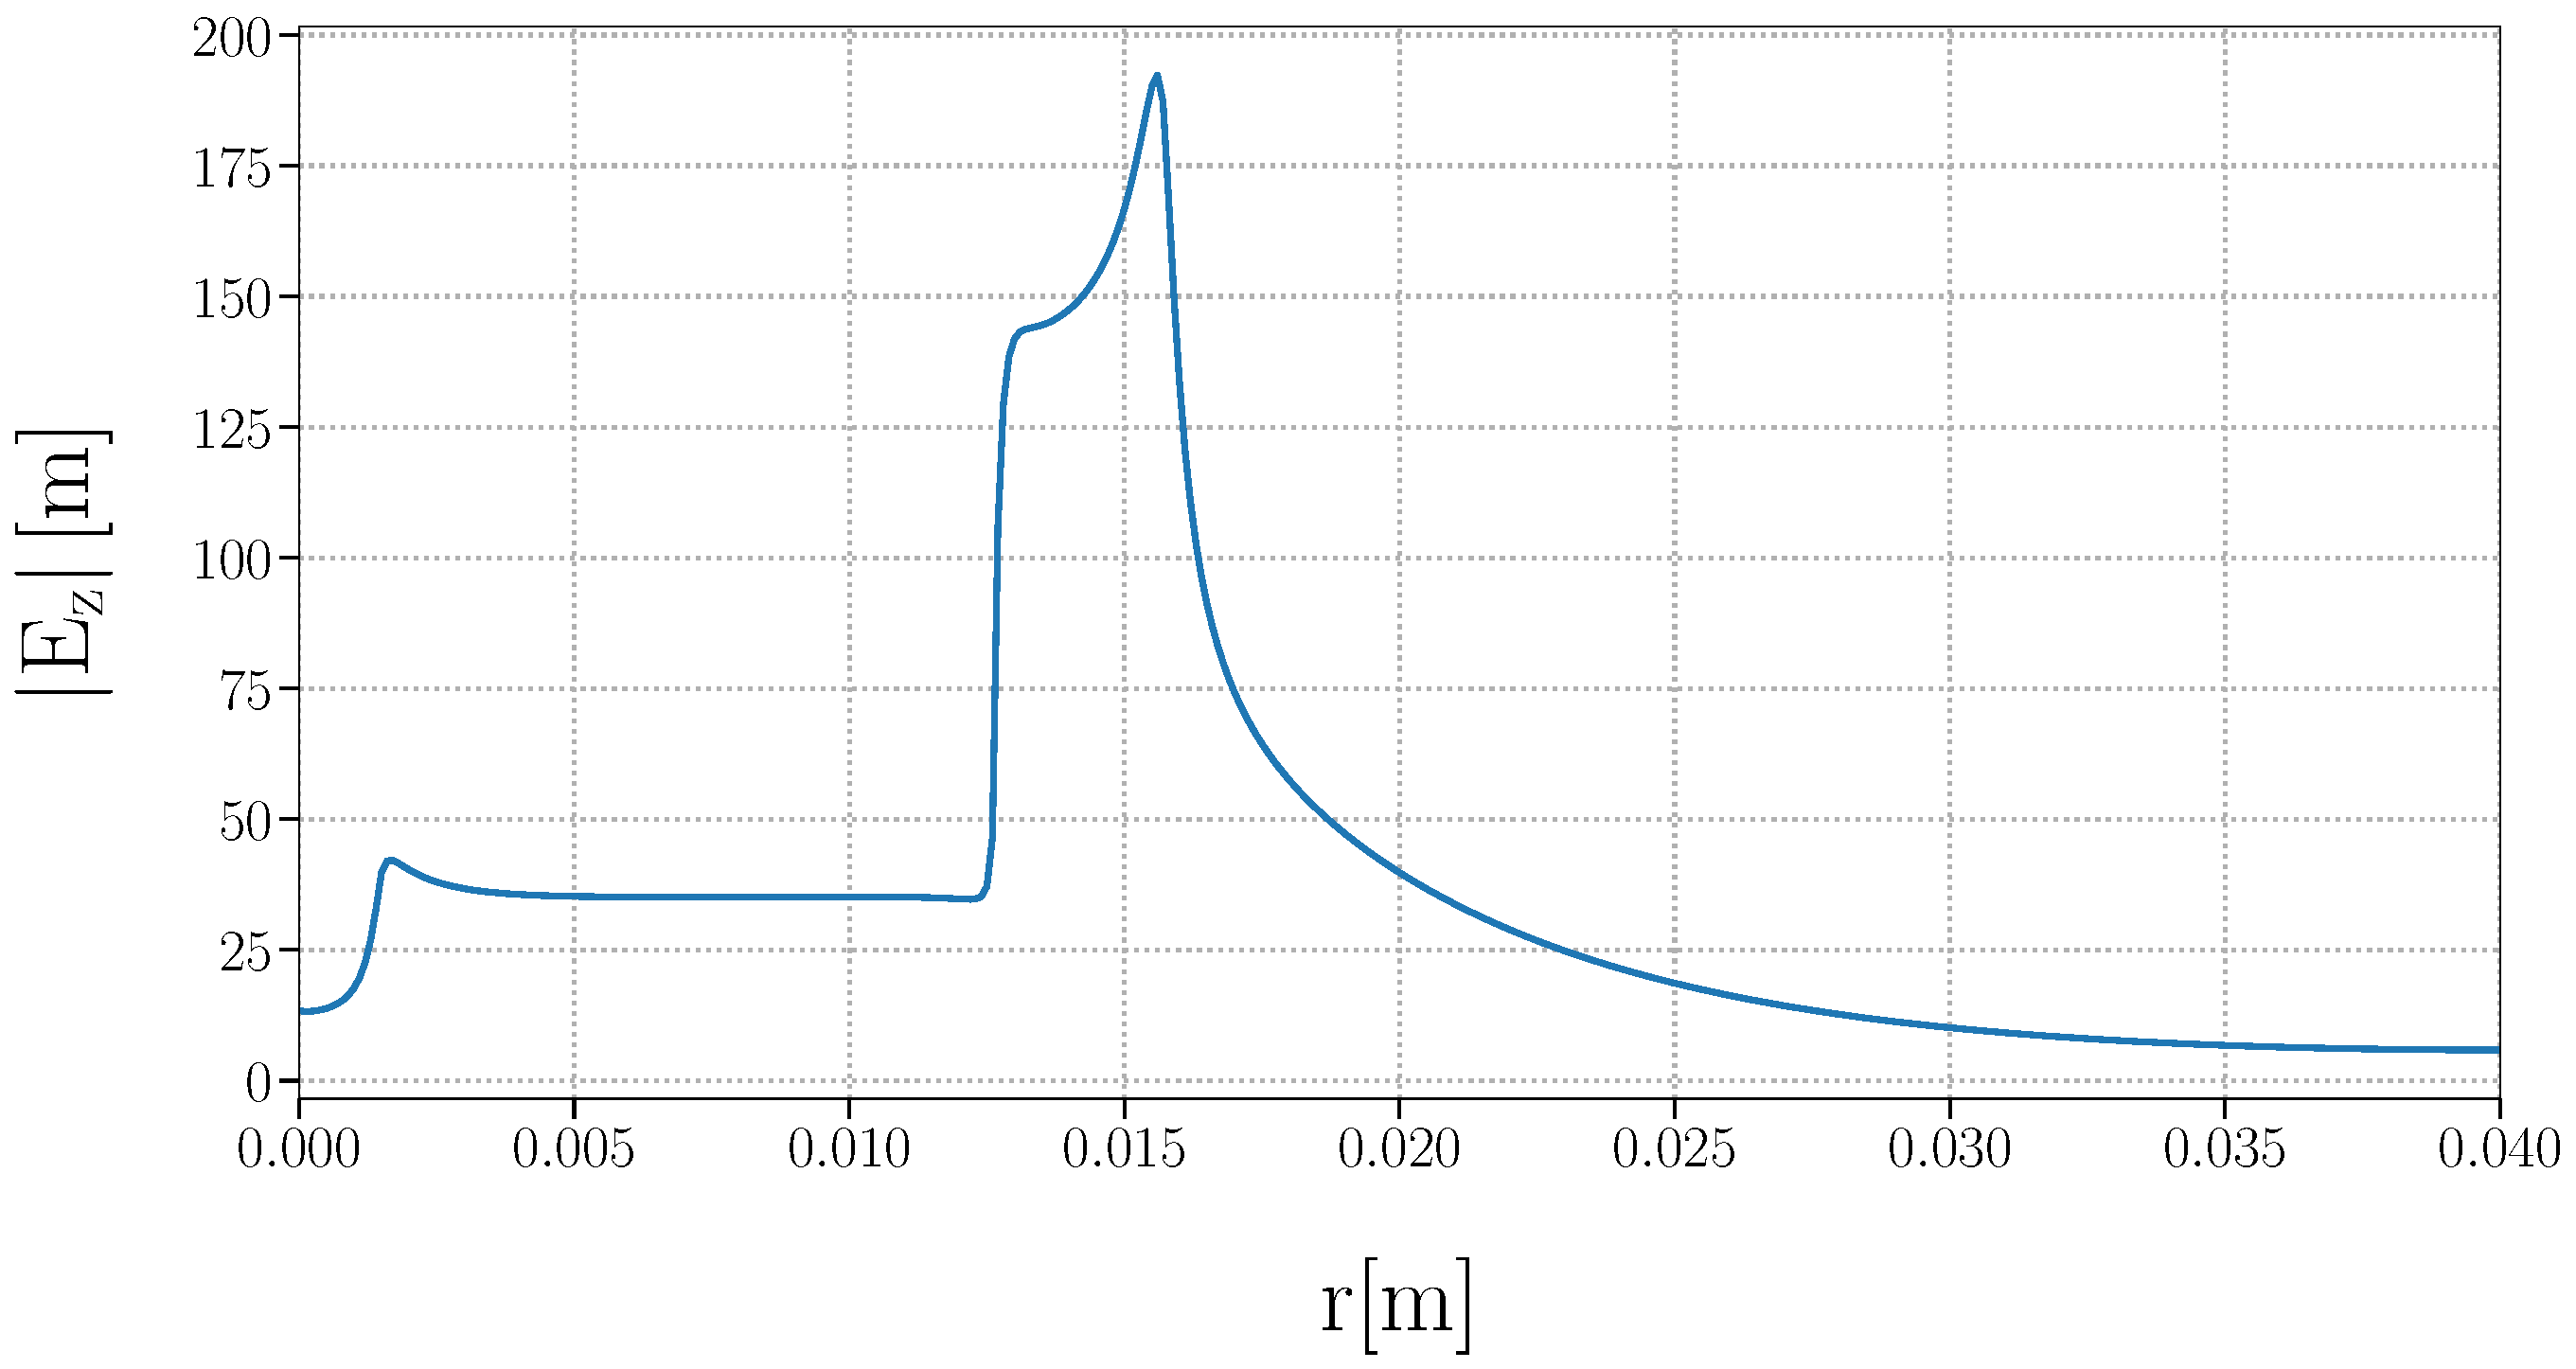
\includegraphics[width=\textwidth]{ALGAAS/fieldxsec_sim.pdf}
    \caption{Plot of the $| \mathrm{E}_\mathrm{z} |$ field cross section sampled about the optic HR coating surface.}
\label{fig:Ez}
\end{figure}

\subsection{Servo Overview}
\begin{figure}[!ht]
	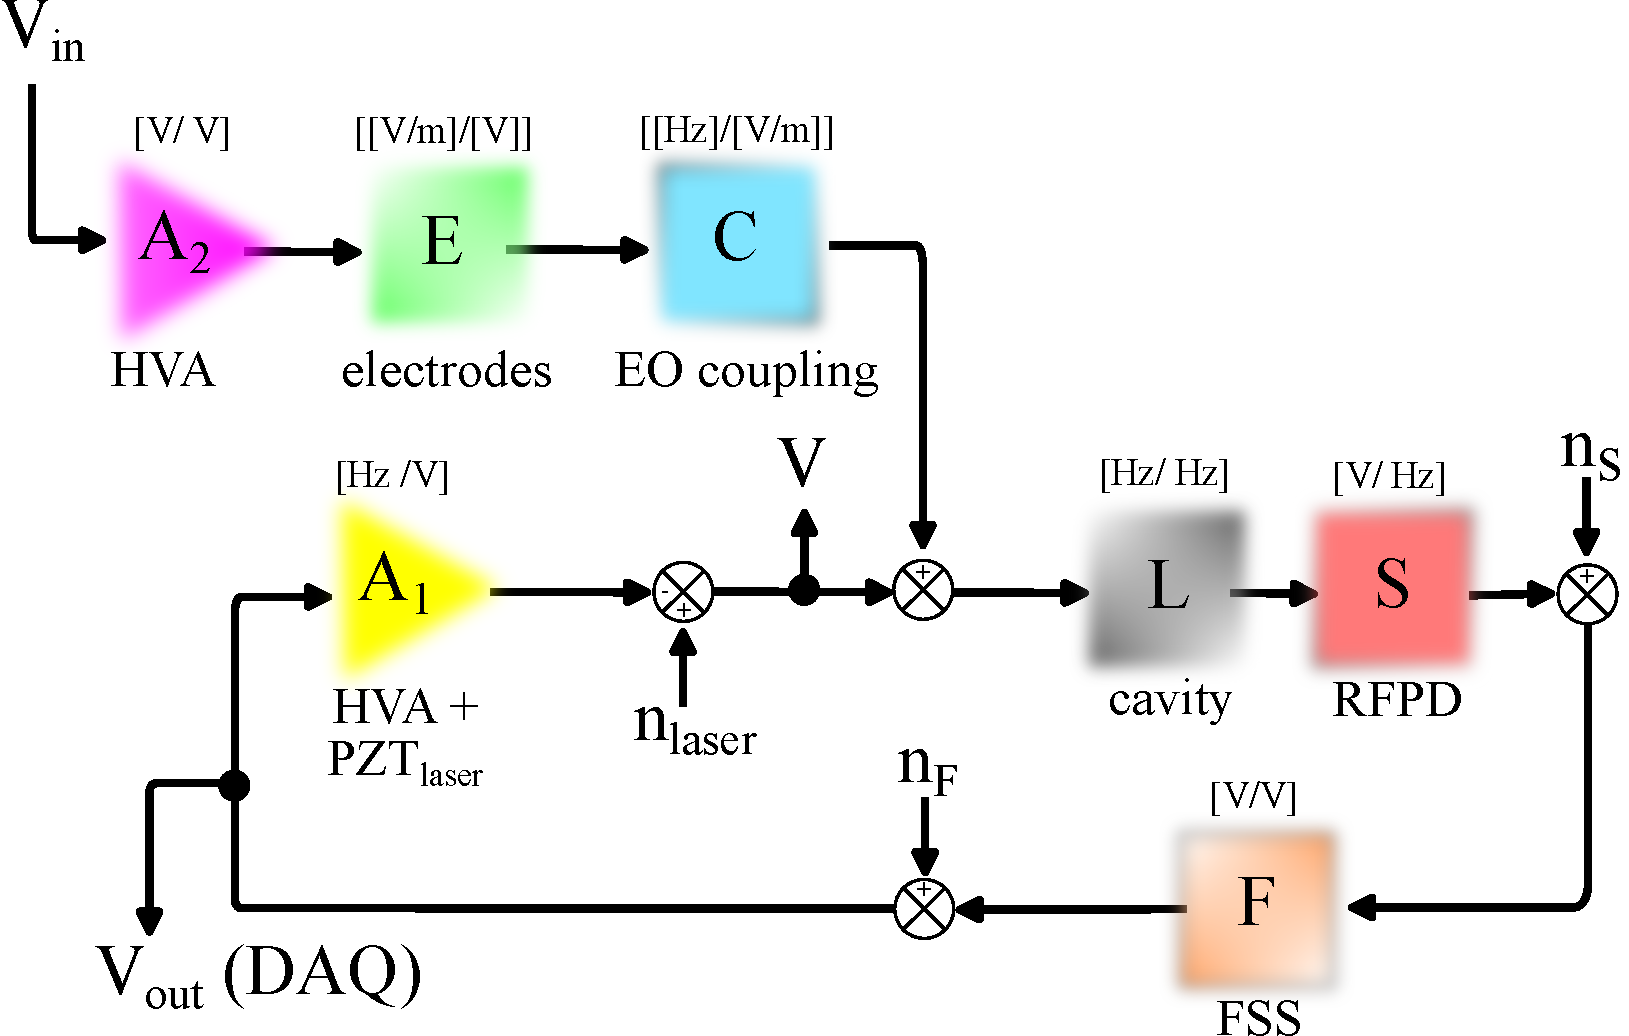
\includegraphics[width=\textwidth]{figs/ALGAAS/pock_control_diagram.pdf}
	\caption{A controls diagram of the designed servo.}
	\label{fig:pock_control_servo}
\end{figure}

\subsection{Calibration}

The Electric field coupling can be expressed as a measured voltage:
$$\mathrm{V} = \frac{1}{1 + \mathrm{G}} \cdot \mathrm{n}_\mathrm{laser} - \frac{\mathrm{G}}{1 + \mathrm{G}} \cdot \mathrm{C}  \cdot \mathrm{E} \cdot \mathrm{A}_{2} \cdot \mathrm{V}_\mathrm{in} - \frac{\mathrm{F} \cdot \mathrm{A}_1}{1 + \mathrm{G}} \cdot \mathrm{n}_\mathrm{S} - \frac{A_1}{1 + \mathrm{G}} \cdot \mathrm{n}_\mathrm{F}$$
With G representing the open loop gain ($\mathrm{G} = \mathrm{A}_1 \cdot \mathrm{F} \cdot \mathrm{S} \cdot \mathrm{L}$). The feedback signal can also be represented as:

	\begin{align*} \mathrm{V}_\mathrm{out} & = \mathrm{F} \cdot \mathrm{S} \cdot \mathrm{L} \cdot (\mathrm{V} + \mathrm{C} \cdot \mathrm{E} \cdot \mathrm{A}_{2} \cdot \mathrm{V}_\mathrm{in}) + \mathrm{F} \cdot \mathrm{n}_\mathrm{S} + \mathrm{n}_\mathrm{F} \\ & = \frac{\mathrm{F} \cdot \mathrm{S} \cdot \mathrm{L}}{ 1 + \mathrm{G}} \cdot \mathrm{C} \cdot \mathrm{E} \cdot \mathrm{A}_{2} \cdot \mathrm{V}_\mathrm{in} + \frac{\mathrm{F} \cdot \mathrm{S} \cdot \mathrm{L}}{ 1 + \mathrm{G}} \cdot \mathrm{n}_\mathrm{laser} + \frac{\mathrm{F} }{ 1 + \mathrm{G}}\cdot \mathrm{n}_\mathrm{S} +  \frac{1}{ 1 + \mathrm{G}} \cdot \mathrm{n}_\mathrm{F} \end{align*}
Therefore, the transfer function ($\frac{\mathrm{V}_\mathrm{out}}{\mathrm{V}_\mathrm{in}}$) : 
$$ \frac{\mathrm{V}_\mathrm{out}}{\mathrm{V}_\mathrm{in}} = \frac{\mathrm{F} \cdot \mathrm{S} \cdot \mathrm{L}}{1 + \mathrm{G}} \cdot \mathrm{C} \cdot \mathrm{E} \cdot \mathrm{A}_{2}  + \frac{\mathrm{F} \cdot \mathrm{S} \cdot \mathrm{L}}{ 1 + \mathrm{G}} \cdot \frac{\mathrm{n}_\mathrm{laser}}{\mathrm{V}_\mathrm{in}}+ \frac{\mathrm{F} }{ 1 + \mathrm{G}} \cdot \frac{\mathrm{n}_\mathrm{S}}{\mathrm{V}_\mathrm{in}} +  \frac{1}{ 1 + \mathrm{G}} \cdot \frac{\mathrm{n}_\mathrm{F}}{\mathrm{V}_\mathrm{in}}$$
If the induced excitation is larger than the noise  we approximate the last equation:

$$ \frac{\mathrm{V}_\mathrm{out}}{\mathrm{V_{in}}} \approx \frac{\mathrm{F} \cdot \mathrm{S} \cdot \mathrm{L}}{1 + \mathrm{G}} \cdot \mathrm{C} \cdot \mathrm{E} \cdot \mathrm{A}_{2} = \frac{\mathrm{G}}{1 + \mathrm{G}} \cdot \mathrm{C} \cdot \mathrm{E} \cdot \frac{\mathrm{A}_{2}}{\mathrm{A}_{1}} $$
 

\iffalse
The calibration math for this measurement explicitly starts with what I
call \(\alpha(f)\) which is a vector of complex numbers that represents
the transfer function \(\mathrm{CH2}(f)/\mathrm{CH1}(f)\) where:

\[\mathrm{CH1}(f) = \mathrm{Source}(f)\] and
\[\mathrm{CH2}(f) = \frac{\mathrm{S}(f)* signal(f)}{1-\mathrm{OLG}(f)}\]

Where \[\mathrm{OLG}(f) = \mathrm{A}(f)* \mathrm{S}(f)\]

and \(signal(f)\) is the demodulated output from
\(\mathrm{RFPD}_\mathrm{refl}\) and \(\mathrm{S}(f)\) is the transfer
function of the frequency stabilization servo.

From here we solve for signal(f):

\[signal(f) = \mathrm{CH2}(f) * \mathrm{A}_{1}(f) * \mathrm{A}_2* \frac{(1-\mathrm{OLG}(f))}{\mathrm{OLG}(f)}\]

Where \(\mathrm{A}_{1}(f)\) informs the frequency dependent drive sent
to the laser PZT to keep the cavity locked and \(\mathrm{A}_2\) is the
laser frequency detuning factor {[}Hz/V{]} (can be estimated from
measuring PDH).

Currently \(signal(f)\) provides a frequency noise spectra which then
can be converted into a displacement spectra with the following
relation:

\[\frac{\Delta f}{f_\mathrm{laser}} = \frac{\Delta L}{L_\mathrm{cav}}\]

This allows us to imagine the frequency noise spectra as a length noise
spectra due to the drive on the electrodes:

\[signal(f) = \alpha(f)* \mathrm{Source}(f) * \mathrm{A}_{1}(f) * \mathrm{A}_2* \frac{(1-\mathrm{OLG}(f))}{\mathrm{OLG}(f)} * \frac{L_\mathrm{cav}}{f_\mathrm{laser}}\hspace{35pt} [m_\mathrm{pk}]\]

And for the measurement normalized by the drive voltage on the
electrodes:

\[\frac{signal(f)}{\mathrm{Source}(f) * \mathrm{G}(f)} = \frac{\alpha(f)}{\mathrm{G}(f)} * \mathrm{A}_{1}(f) * \mathrm{A}_2* \frac{(1-\mathrm{OLG}(f))}{\mathrm{OLG}(f)} * \frac{L_\mathrm{cav}}{f_\mathrm{laser}}\hspace{35pt} \bigg[\frac{m_\mathrm{pk}}{V_\mathrm{pk}}\bigg]\]
\#\# Noise or single frequency drive measurement : \(n(f)\) The
calibration math for this measurement is essentially equivalent to the
transfer function measurement above. The only difference is:

\[\mathrm{CH1}(f) = \frac{\mathrm{S}(f)* signal(f)}{1-\mathrm{OLG}(f)}\]

and

\[signal(f) = \mathrm{CH1}(f) * \mathrm{A}_{1}(f) * \mathrm{A}_2* \frac{(1-\mathrm{OLG}(f))}{\mathrm{OLG}(f)} * \frac{L_\mathrm{cav}}{f_\mathrm{laser}}\]

Where \(signal(f)\) in this measurement represents the free running
cavity displacement noise with the exception of a single frequency if it
is not a noise measurement.

If \(\mathrm{CH1}(f)\) is in \(\frac{V_\mathrm{rms}}{\sqrt{Hz}}\) then
signal(f) will be in \(\frac{m_\mathrm{rms}}{\sqrt{Hz}}\)

or

If \(\mathrm{CH1}(f)\) is in \(V_\mathrm{pk}\) then signal(f) will be in
\(m_\mathrm{pk}\) 
\fi

%\#\# Calibration code
%The error signal spectra probed at the FSS:
%\begin{equation}
%\mathrm{VFSSOUT}_\mathrm{rms}/\sqrt{Hz} \rightarrow m_\mathrm{rms}/\sqrt{\mathrm{Hz}}
%\end{equation}
%With the known frequency response of the servo electronics, we \autoref{sec:calibration} the measurement into differential length:
%\begin{equation}
%	\Delta \mathrm{L} = \mathrm{source}*\alpha(f) \mathrm{A}(f)*\frac{1+\mathrm{OLG}(f)}{\mathrm{OLG}(f)}*\frac{\mathrm{L_{cav}}}{f_\mathrm{laser}} \quad \big[ m_\mathrm{pk} / \sqrt{Hz} \big]
%\end{equation}

\subsection{Assembly Mount Solution}
%The following section details measurements performed with various longitudinal pockel cell mounts. Further details (assembly parameters, blueprints, and visual aids) can be found in the appendix.
%\subsubsection{Assembly 3 (MACOR mount)}
To maintain the aforementioned boundary conditions in situ, an optical mount made of MACOR, a machinable ceramic, was constructed and installed. With the material's high Young's modulus (66.9 GPa), and a moderate Poisson ratio (.29) \cite{macor} making it by far the most durable / non-conductive mounting solution tried.

An optical mount for the sample made with MACOR, along with spherical glass bearnings with a .48 $\pm$ .01 cm $\diameter$, and a McMaster-Carr 8-32, 1/2" ceramic screw were used to clamp the optical sample within a bored 25.74 $\pm$ .5 mm $\diameter$ barrel. Two 1.24" $\diameter$ holes were also bored at a 9 mm depth about the front and back side of the optical mount to accomodate for a flush fit of copper electrodes. The construction suggests a 1 $\pm$ .5 mm clearance between the front and back surface of the sample to the electrode plates.

%%FIGURE: sample in-situ
\begin{figure}[!ht]
    \begin{subcaptiongroup}
	    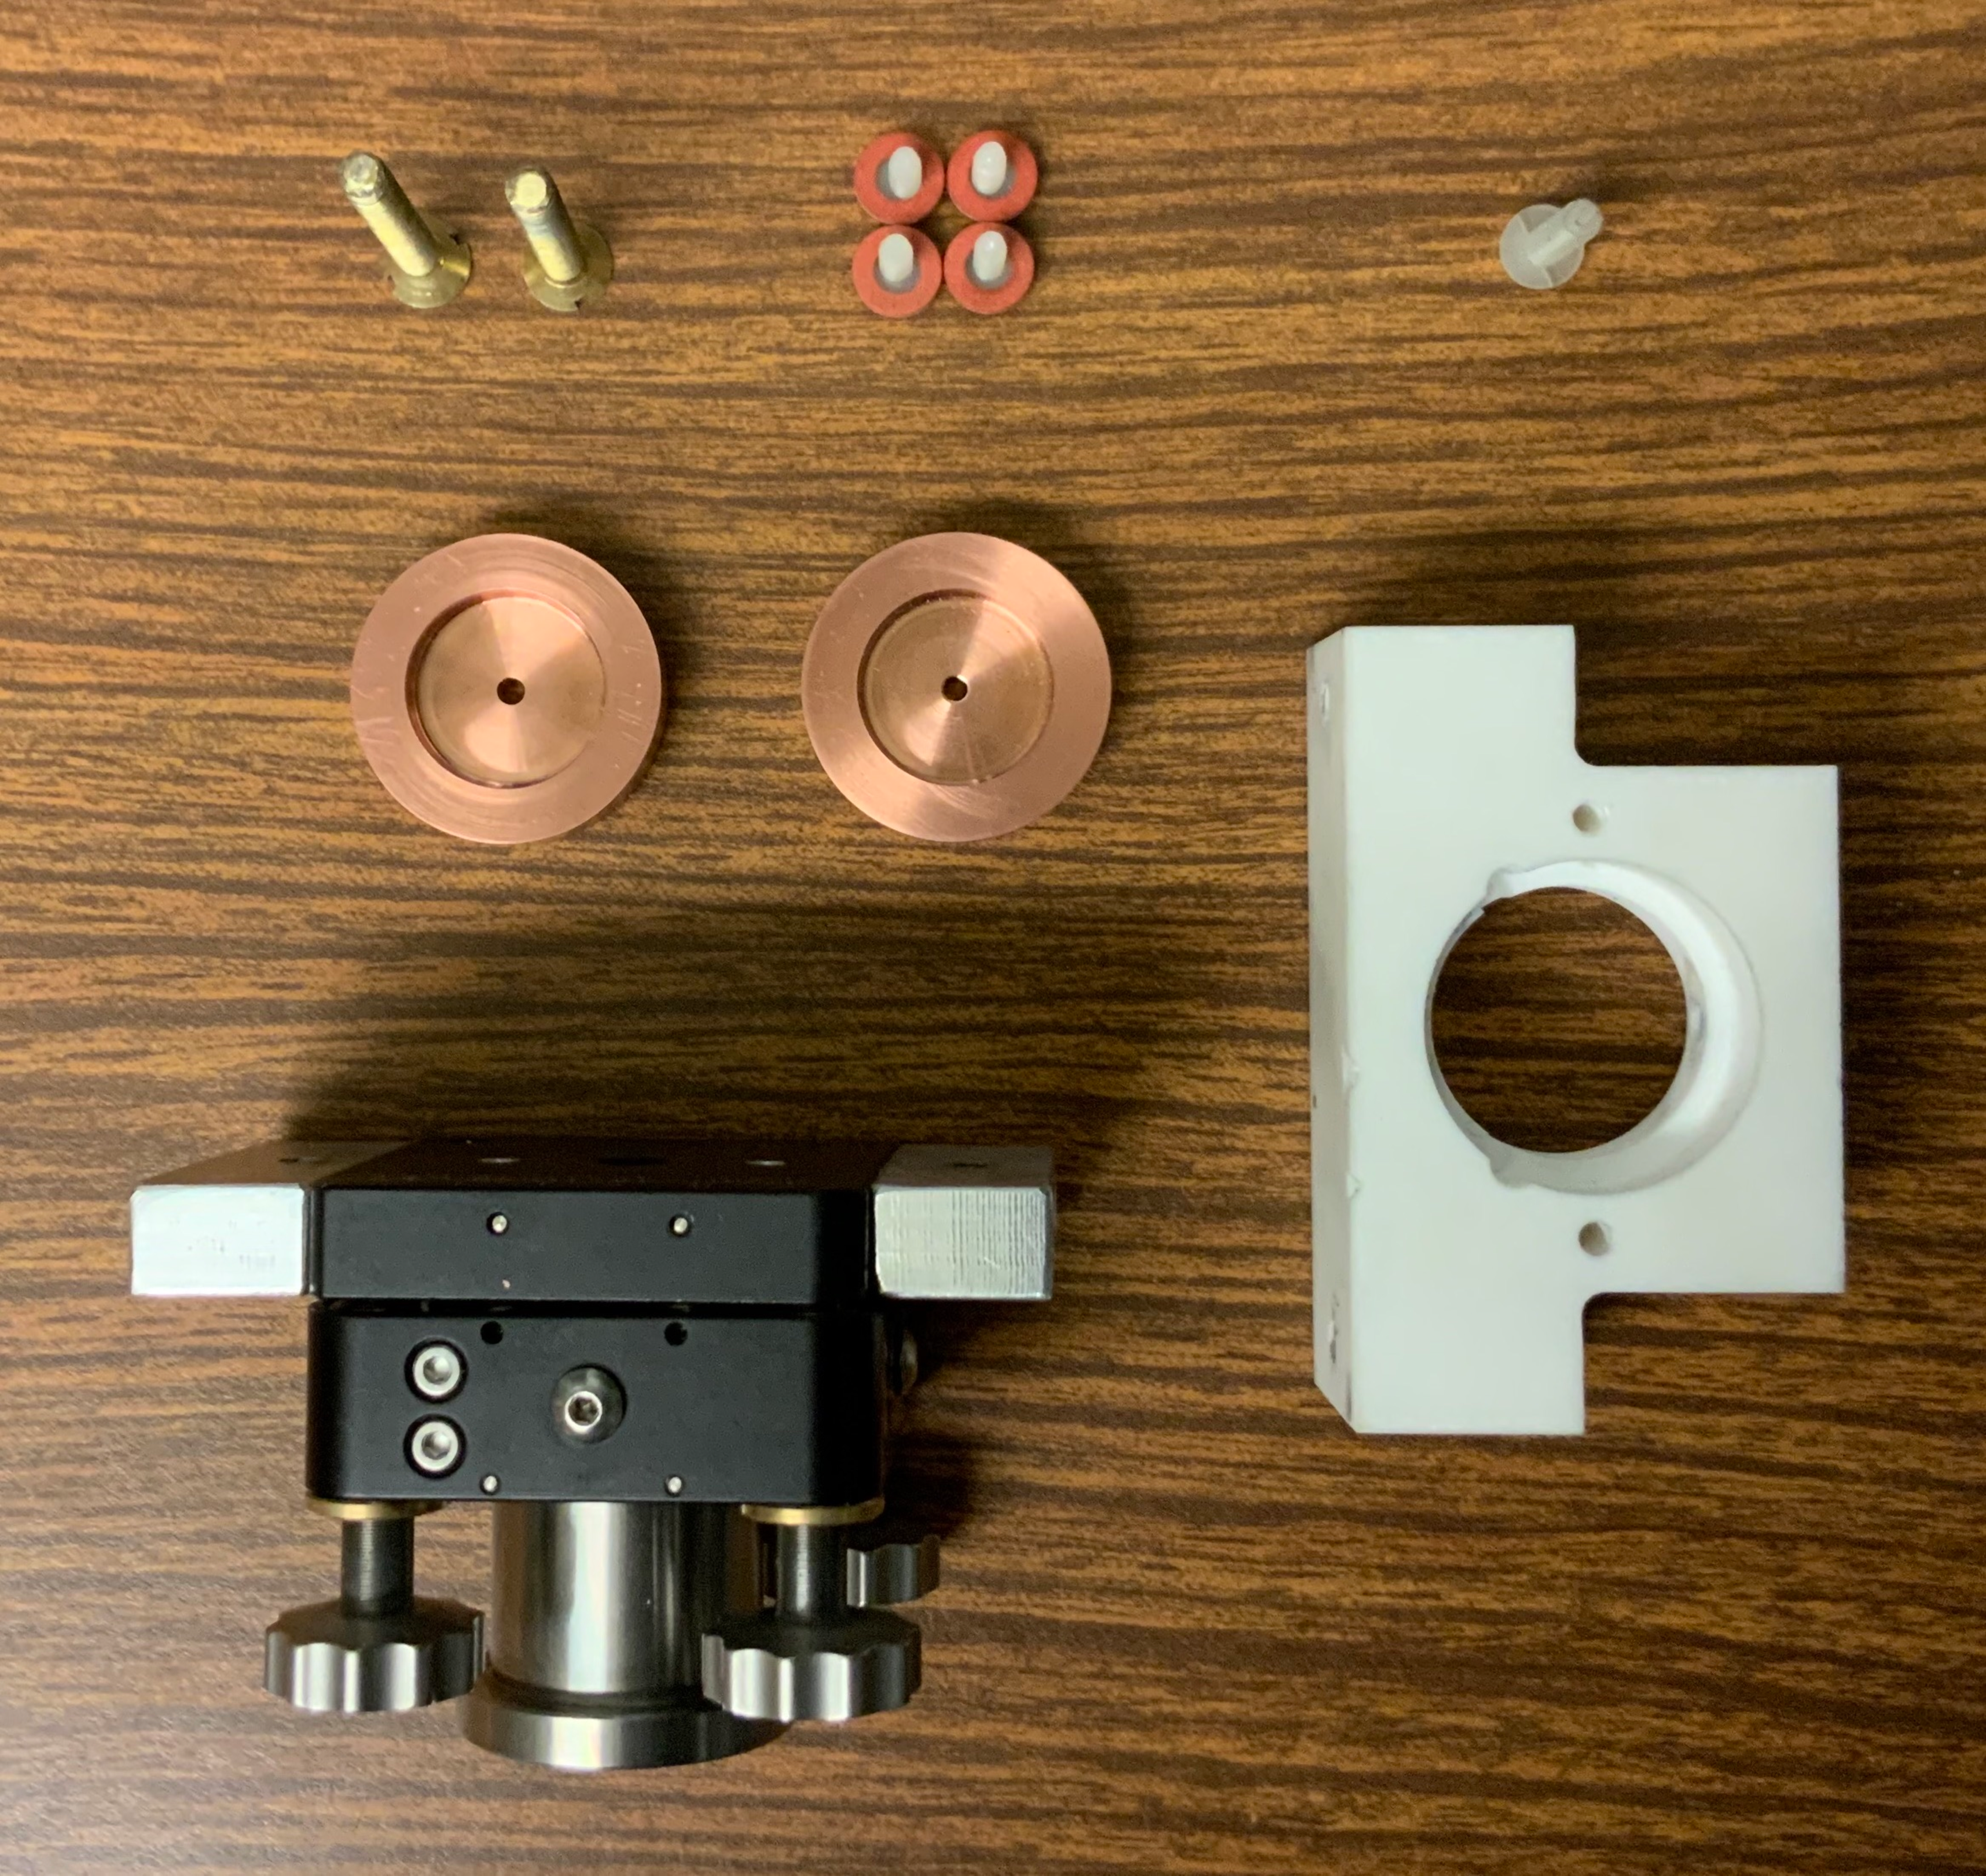
\includegraphics[width=.5\textwidth]{figs/ALGAAS/assemblies/assembly3/assembly3_disassembled.pdf}
	    \phantomcaption\label{subfig:A3disassembled}
	    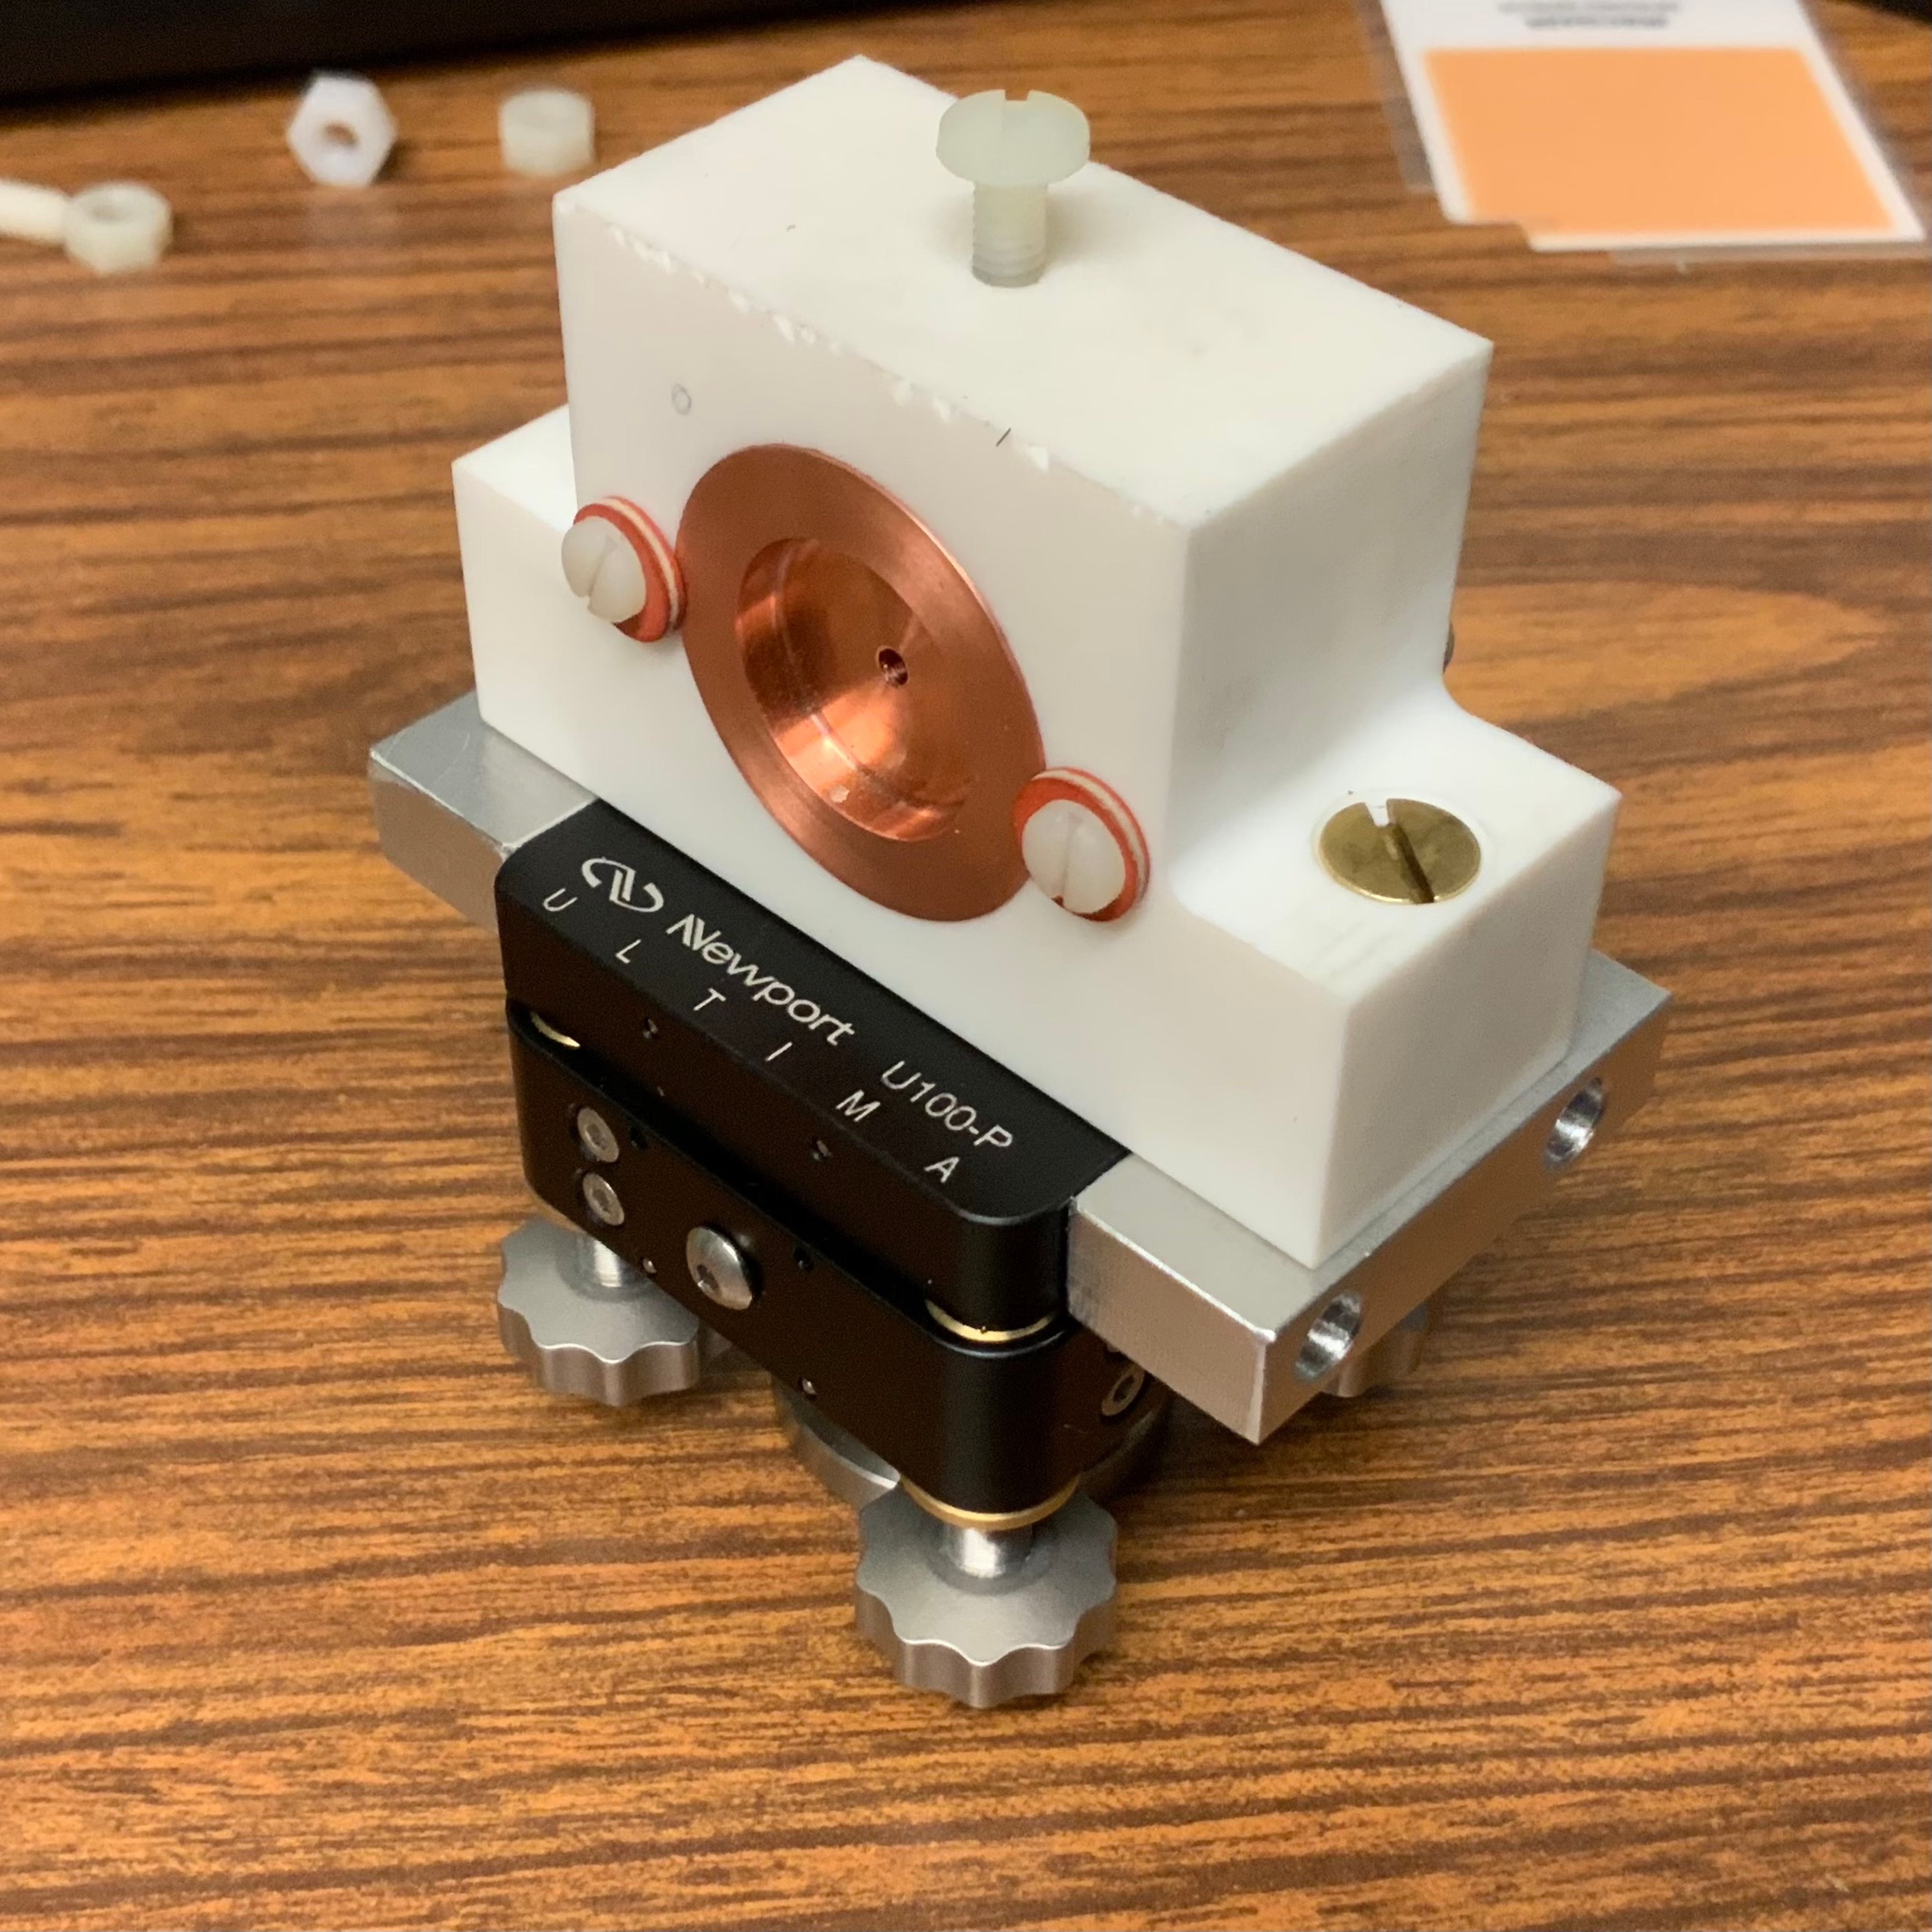
\includegraphics[width=.472\textwidth]{figs/ALGAAS/assemblies/assembly3/assembly3_isometric.pdf}
	    \phantomcaption\label{subfig:A3isometric}
    \end{subcaptiongroup}
    \caption{Assembly 3: \subref{subfig:A3disassembled} disassembled configuration and \subref{subfig:A3isometric} an isometric view of the assembled configuration.}
    \label{fig:assembly3}
\end{figure}


\begin{figure}[H]
    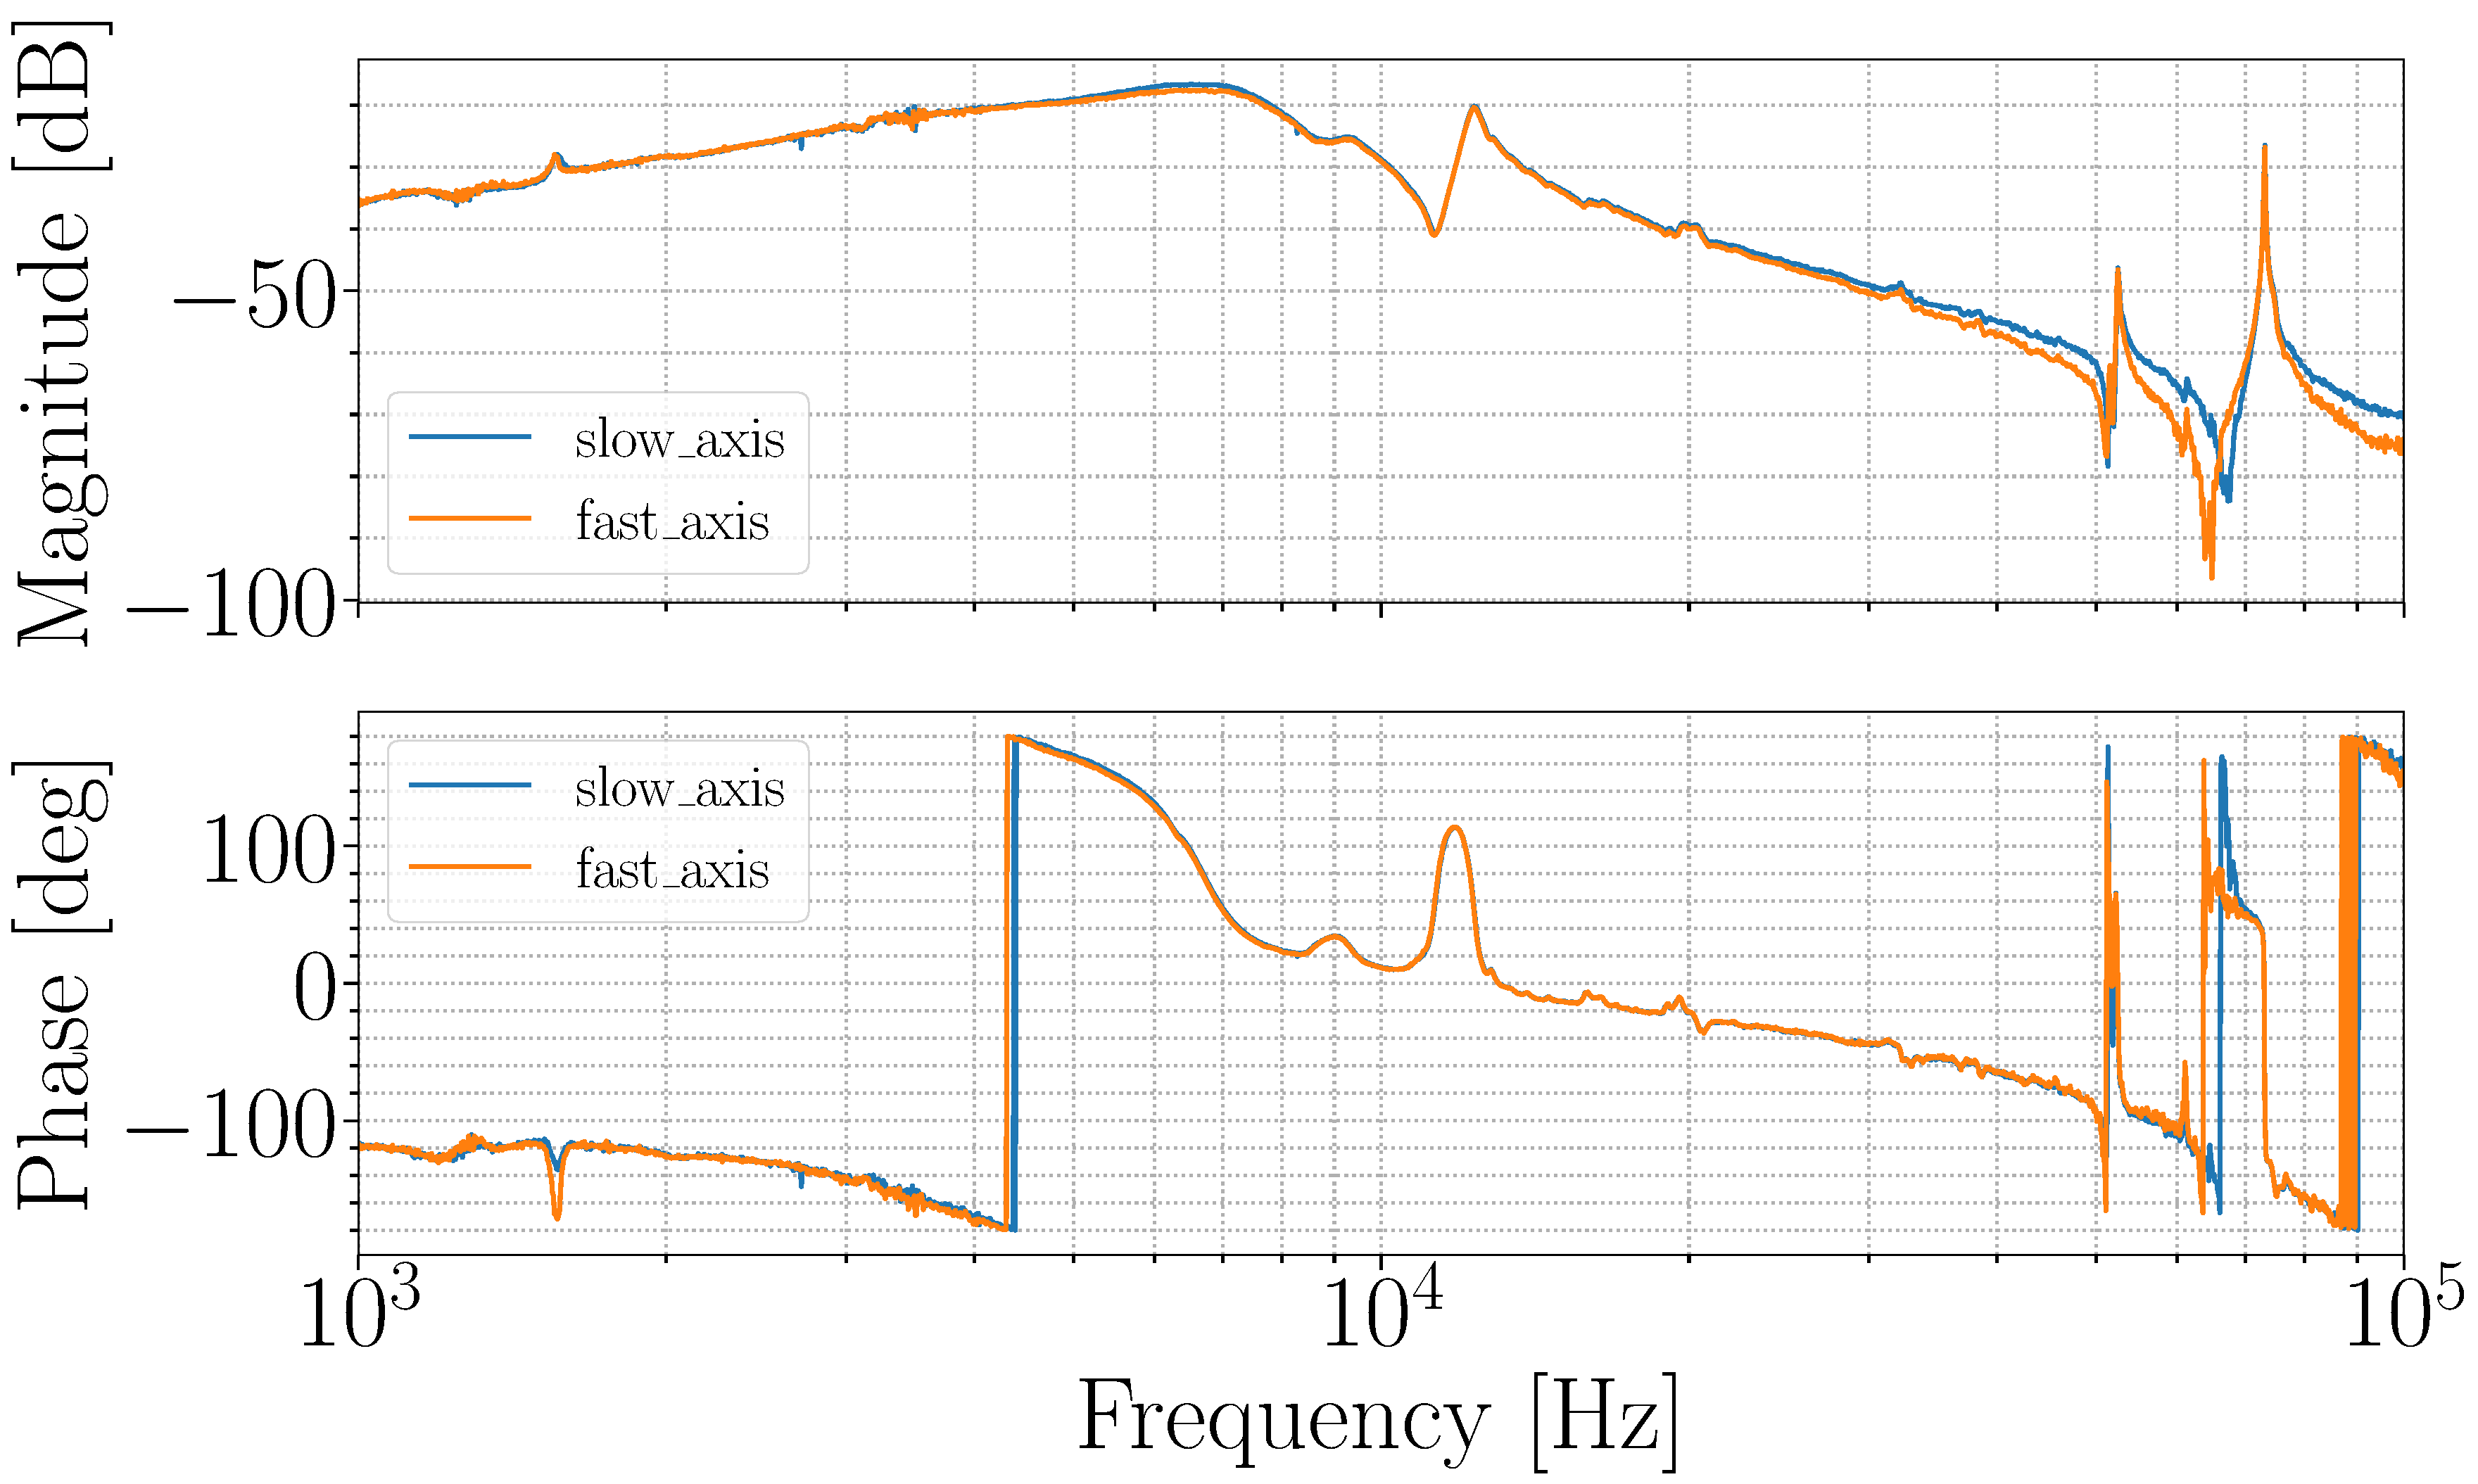
\includegraphics[width=\textwidth]{figs/ALGAAS/rawtf_fast_slow.pdf}
    \caption{Uncalibrated measurement with the polarization aligned along the slow and fast $\gaas$ / $\algaas$ coating axes using the MACOR mount}
    \label{fig:rawtf_fast_slow}
\end{figure}


\subsection{Measured birefringence from HR \texorpdfstring{$\gaas$}{gaas}/\texorpdfstring{$\algaas$}{algaas} mirror}

To identify the fast and slow axes, the crystalline HR mirror is temporarily paired with a highly reflective input mirror to form a high finesse cavity. The DC power in reflection of the cavity was probed while the laser frequency was linearly swept about resonance and various input laser polarizations sampled using a half waveplate ($\lambda$ / 2). The resulting measurements exhibit a split cavity resonance when the beam polarization is not co-aligned with one of the two eigenaxes set by the HR sample birefringence.

\begin{figure}
    \centering
    \begin{subfigure}{.48\linewidth}
	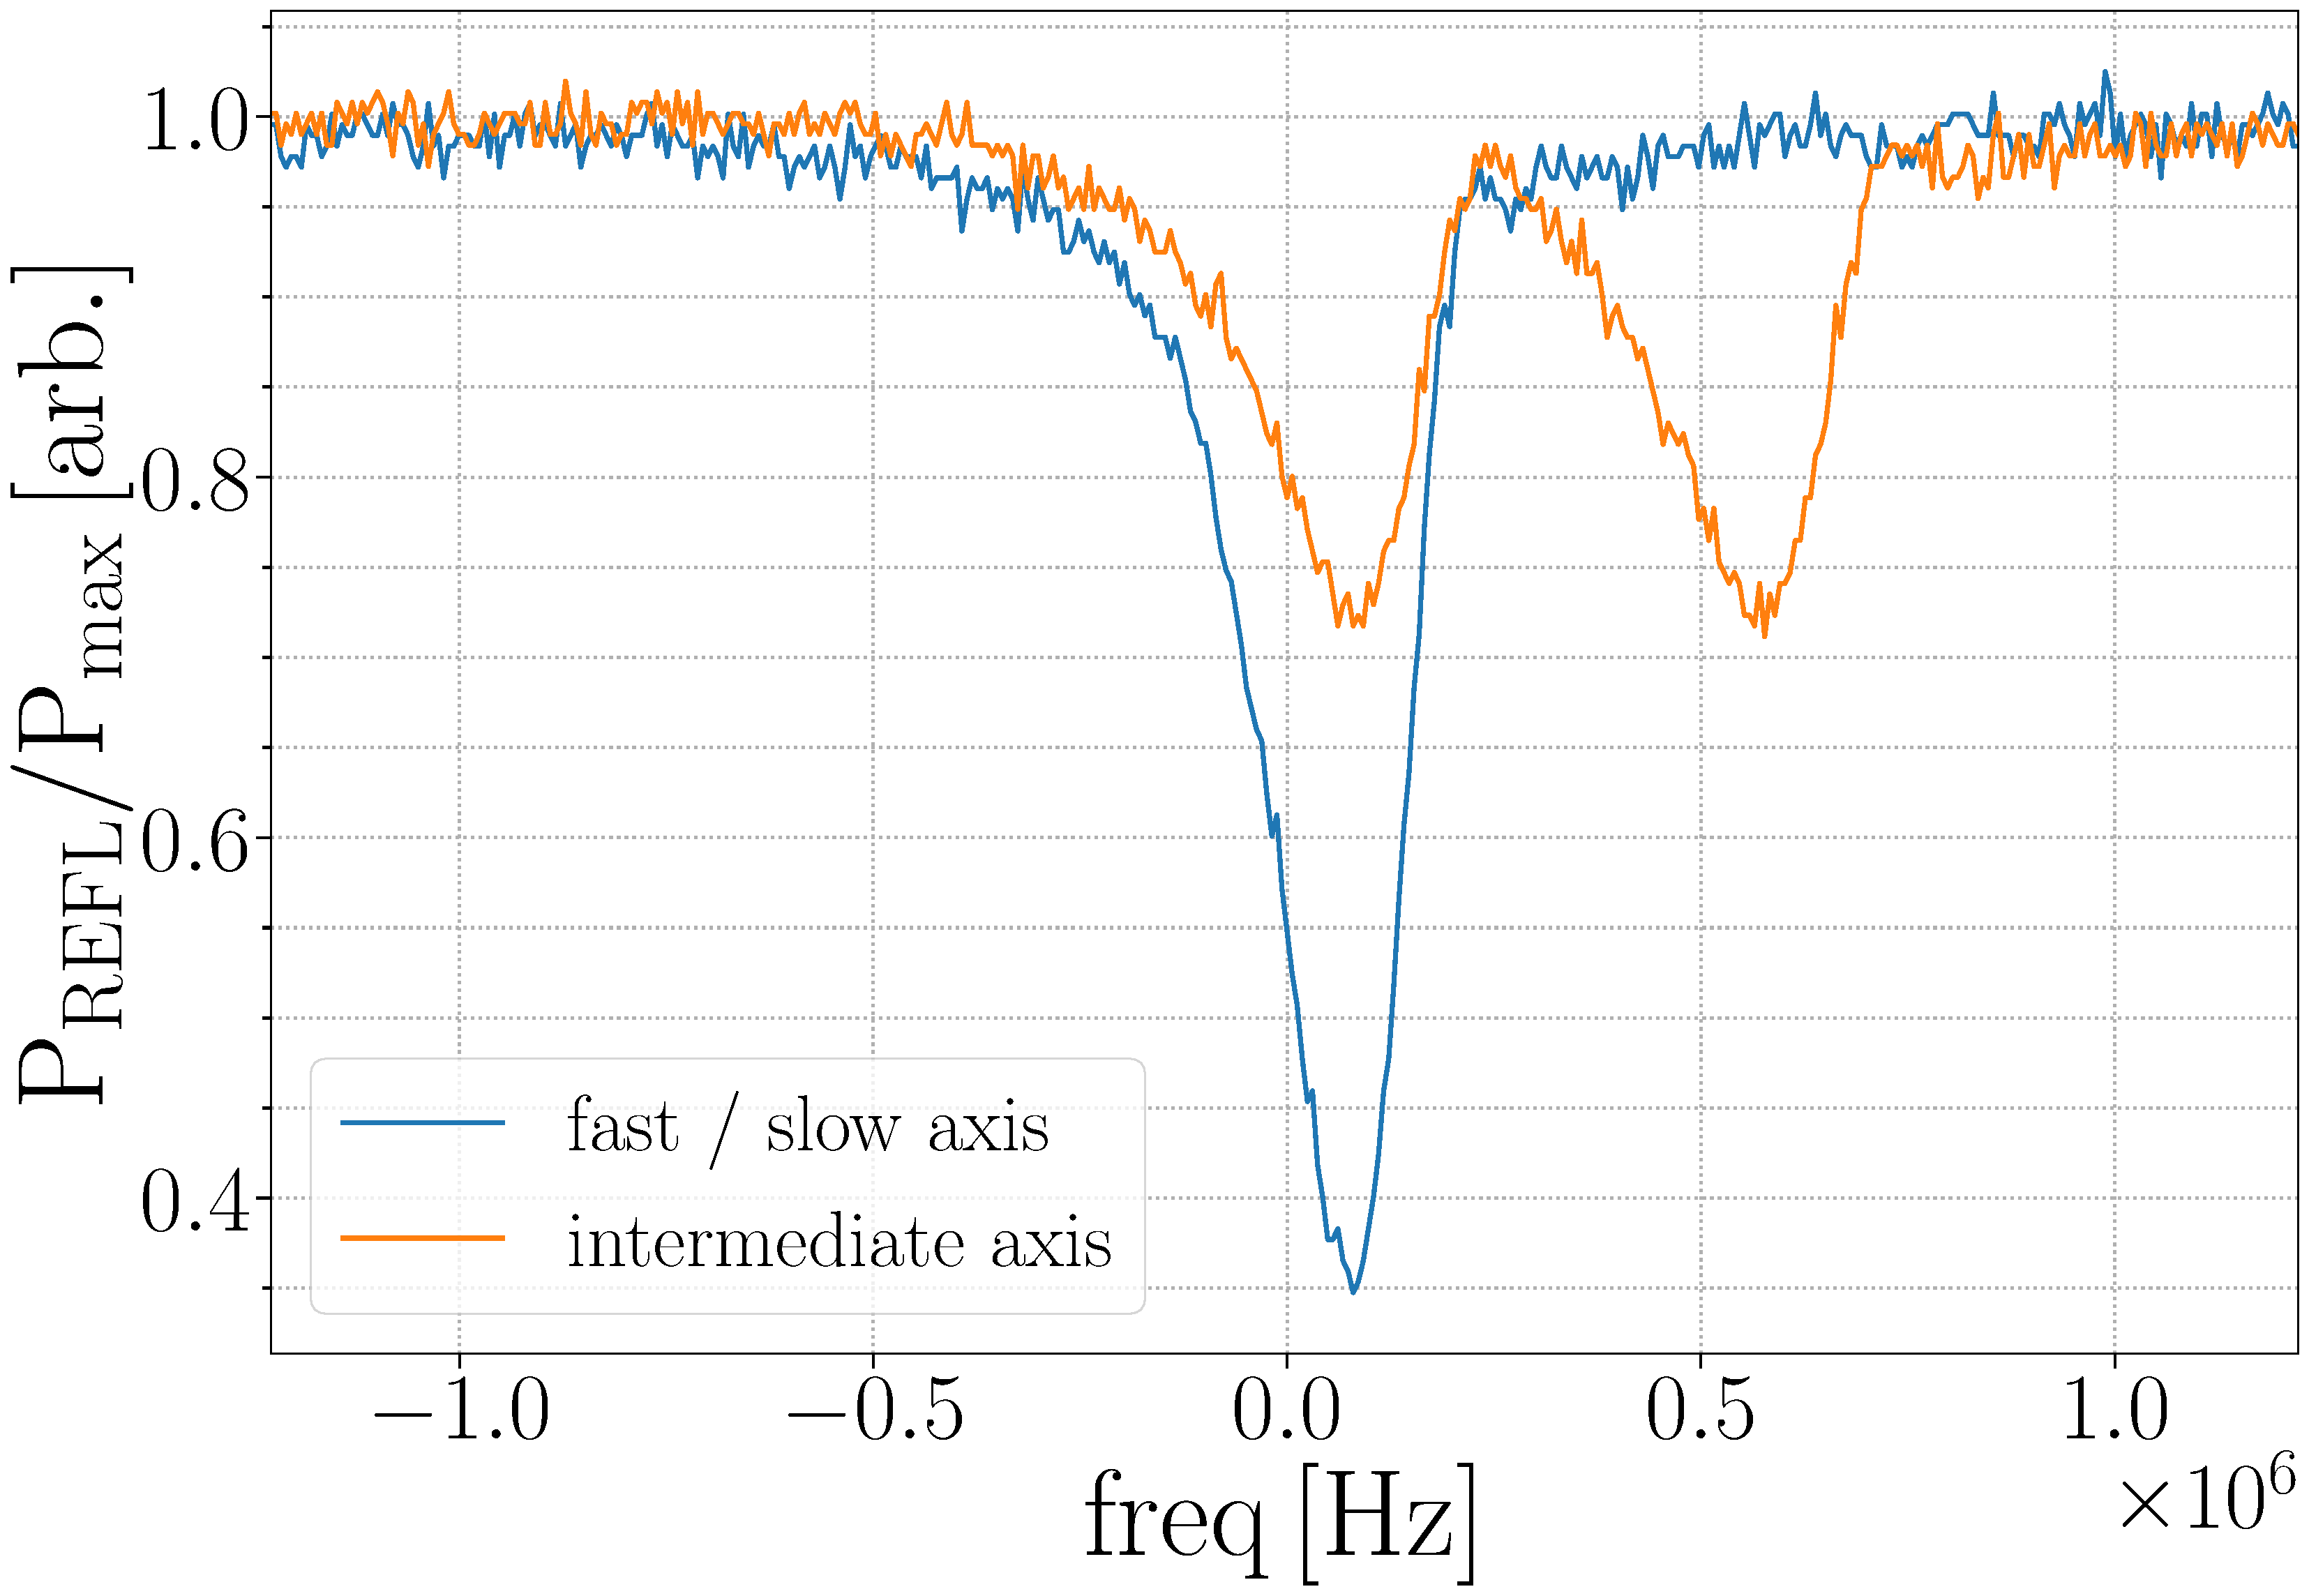
\includegraphics[width=\linewidth]{figs/ALGAAS/split_cav_scan.pdf}
	\label{splitresonance}
    \end{subfigure}
    \begin{subfigure}{.50\linewidth}
	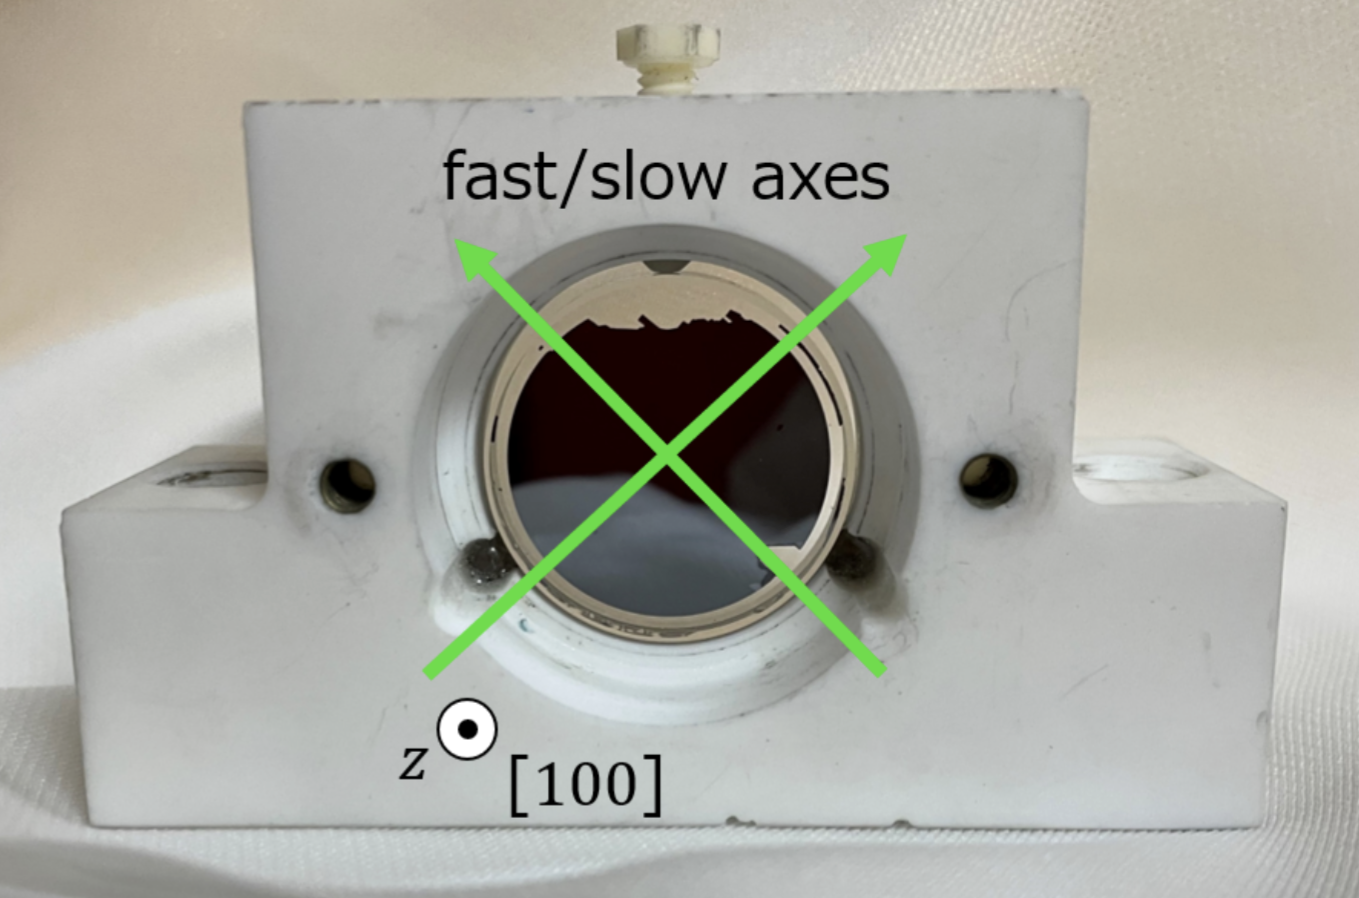
\includegraphics[width=\linewidth]{figs/ALGAAS/fas_axes.png}
	\label{fast_slow_axes}
    \end{subfigure}
    \caption{[Right] Lines running parallel to fast and slow axes. It was understood prior that a flat would be normal to one of the two eigenaxes. Measurement of the split resonance [Left] suggests no flat to be present and the damage seen is due to excessive handling. This split has the indicated frequency separation of 500 kHz.}
    \label{fig:split_cav_resonance}
\end{figure}

\begin{figure}[!h]
    \centering
    \begin{subcaptiongroup}
	    \includegraphics[page=2,width=.325\textwidth]{ALGAAS/laser_mirror_algaas_coat_defect.pdf}
	    \phantomcaption\label{conormaldefect}
	    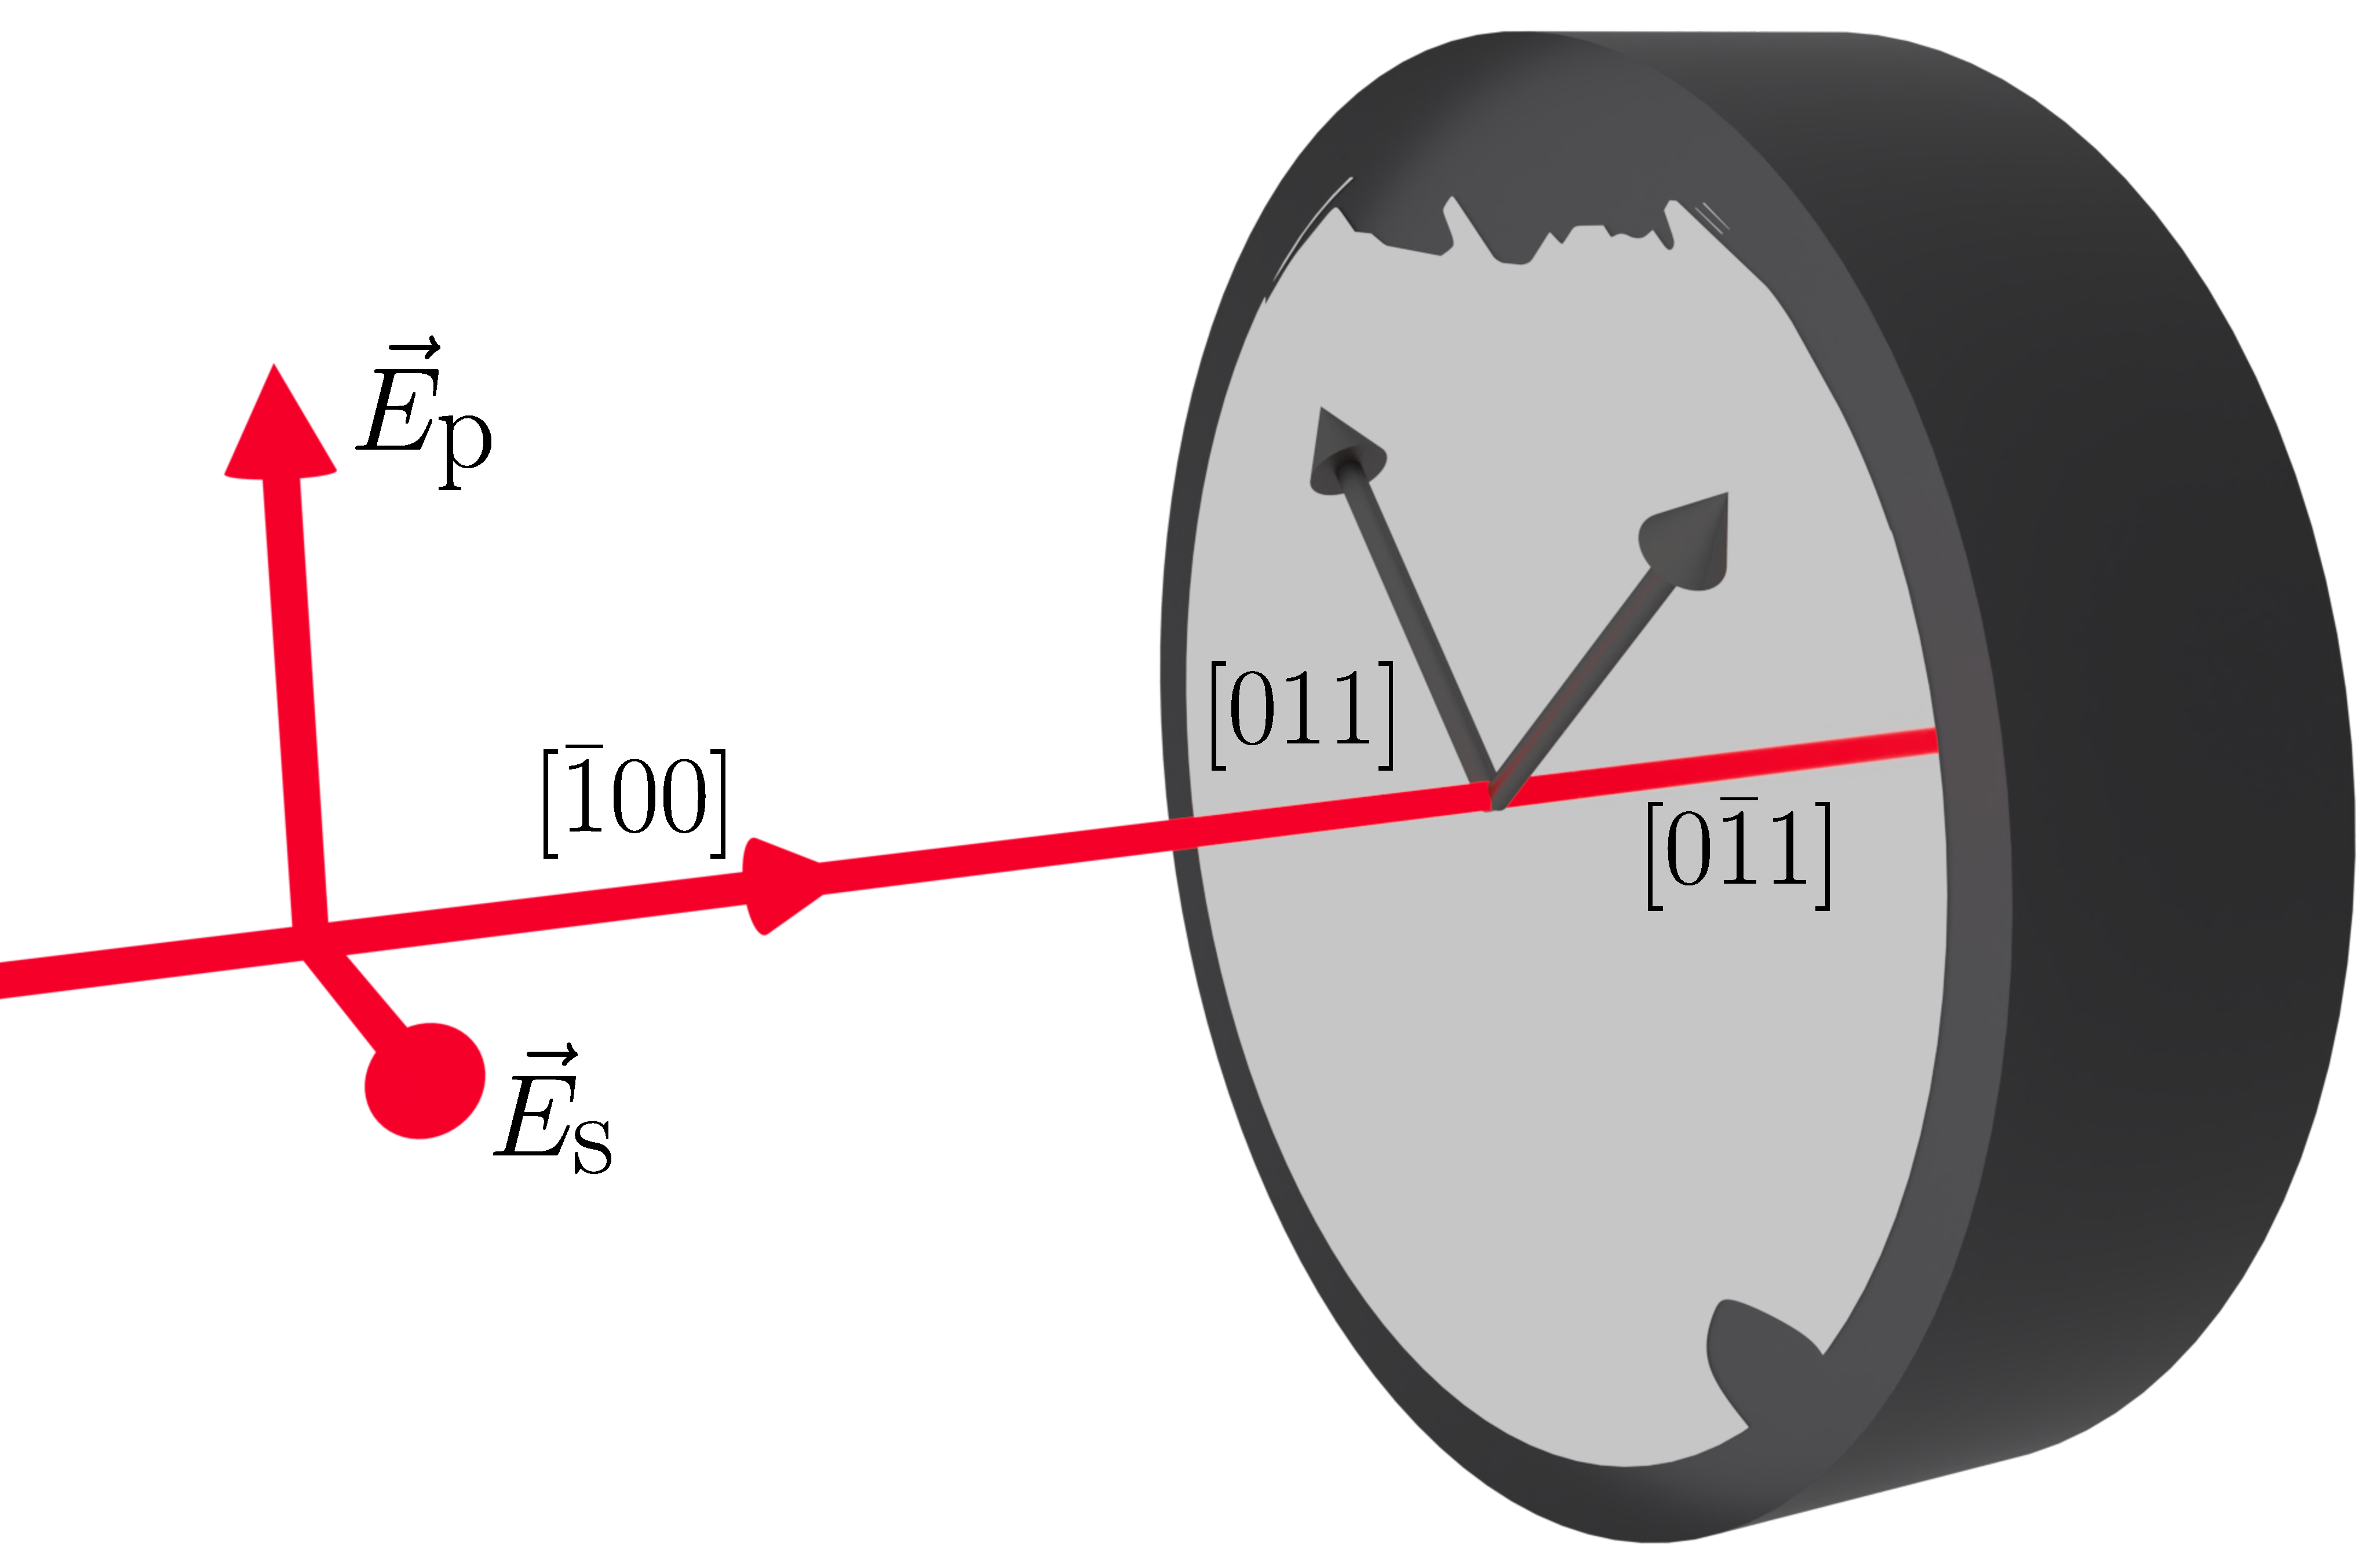
\includegraphics[page=1,width=.5\textwidth]{ALGAAS/laser_mirror_algaas_coat_defect.pdf}
	    \phantomcaption\label{coisodefect}
    \end{subcaptiongroup}
    \caption{Input beam orientation with respect to the coating miller indices / fast and slow axes, with a [Left] Normal view and [Right] isometric view.}
\end{figure}


%There are different accounts of a measured birefringence from HR $\gaas$ / $\algaas$ coatings (\href{https://dcc.ligo.org/DocDB/0181/G2200386/001/G2200386.pdf}{Satoshi}, \href{https://nodus.ligo.caltech.edu:8081/CTN/1474}{CTN}, \href{https://dcc.ligo.org/DocDB/0181/G2200559/001/G2200559-v1\%20-\%20polarization.pdf}{Aidan})
%%Is the measured birefringence static? (Layer bonding method might introduce something?)
%% Does it change from different mounting methods? (Photoelastic) (order of magnitude estimate)
%% Electro-optic ruled out based on field measurements and relative coupling factor.
%% Measurement precision of the coating birefringence? Cavity length, Polarization drifts, etc.
From coating manufacturers it's estimated that static birefringence can arise from the intrinsic strain between hetero-epitaxial layers of $\gaas$/$\algaas$. \cite{cole:2013, adachi:1985}

\section{Results}

\subsection*{Acousto-optical coupling}
A significant barrier to a low cavity differential length noise was encountered when mounting the optics in accessible non-conductive materials. Firstly, most commercial optical mounts are constructed with conductive materials which proves problematic when working to isolate the coating from non-normal field gradients within the coating volume of interest. For this reason, efforts were focused on developing a suitable mounting solution that would provide adequate isolation from any uncontrolled field magnitudes while driving a field normally incident on the surface with enough strength and uniformity across the beam area to extract a measurement of the differential length change from the Pockels effect. The mounts studied span different geometries and different material properties. The varying geometrical assemblies rendered various responses and for this reason some discussions are divided accordingly. A hard lesson learned (while the answer being readily available in collaboration literature) was to select a material that tend towards narrow acoustic resonances while achieving low noise off resonance and at a bandwidth of interest. The most stable solution revealed that ringing of the sample acoustic modes may be responsible For reassurance, we compare displacement spectra against that of a nearly identical cavity with a flat non-crystalline mirror coating to perform a null measurement reference; ruling out the Pockels effect and providing information for noise investigations.


Varying the mechanical configurations (i.e. differential electrode and / or optic set screw settings) to the slightest degree left us to discover a mechanical action via the excitations from the sample-mount acoustic modes from the construction are rung when driving the voltage on electrodes plates. Tracking consistent mechanical action for assemblies prior to Assembly 3 were difficult due to inconsistencies in mechanical settings between some measurements. When more consistency was realized (i.e. utilizing a MACOR mount and careful tracking of the sample set screw torque), it was more transparent that the sample-mount acoustic modes were responsible with similar features between the $\gaas$/$\algaas$ coating and the non-crystalline HR coating from ATFilms. The cleanest versions of these measurements with coorespondence of FEA suggest the acousto-optical modes with highest contributions of cavity length noise at regions below 10 kHz and 40 kHz - 80 kHz. Drive coupling seen in the transfer function measurements with the MACOR mounts appeared consistent. The transfer function differential between fast and slow axes provides an upper threshold estimate:

\[ 
    \begin{aligned}
	\mathrm{diff} & = C_\mathrm{slow} - C_\mathrm{fast} \\
		      & = (C_\mathrm{m, slow} + C_\mathrm{EO, slow}) - (C_\mathrm{m, fast} + C_\mathrm{EO, fast}) \\
		      & =  2 |C_\mathrm{EO}| e^{i \psi}
    \end{aligned}
\]

\begin{figure}[H]
    \centering
    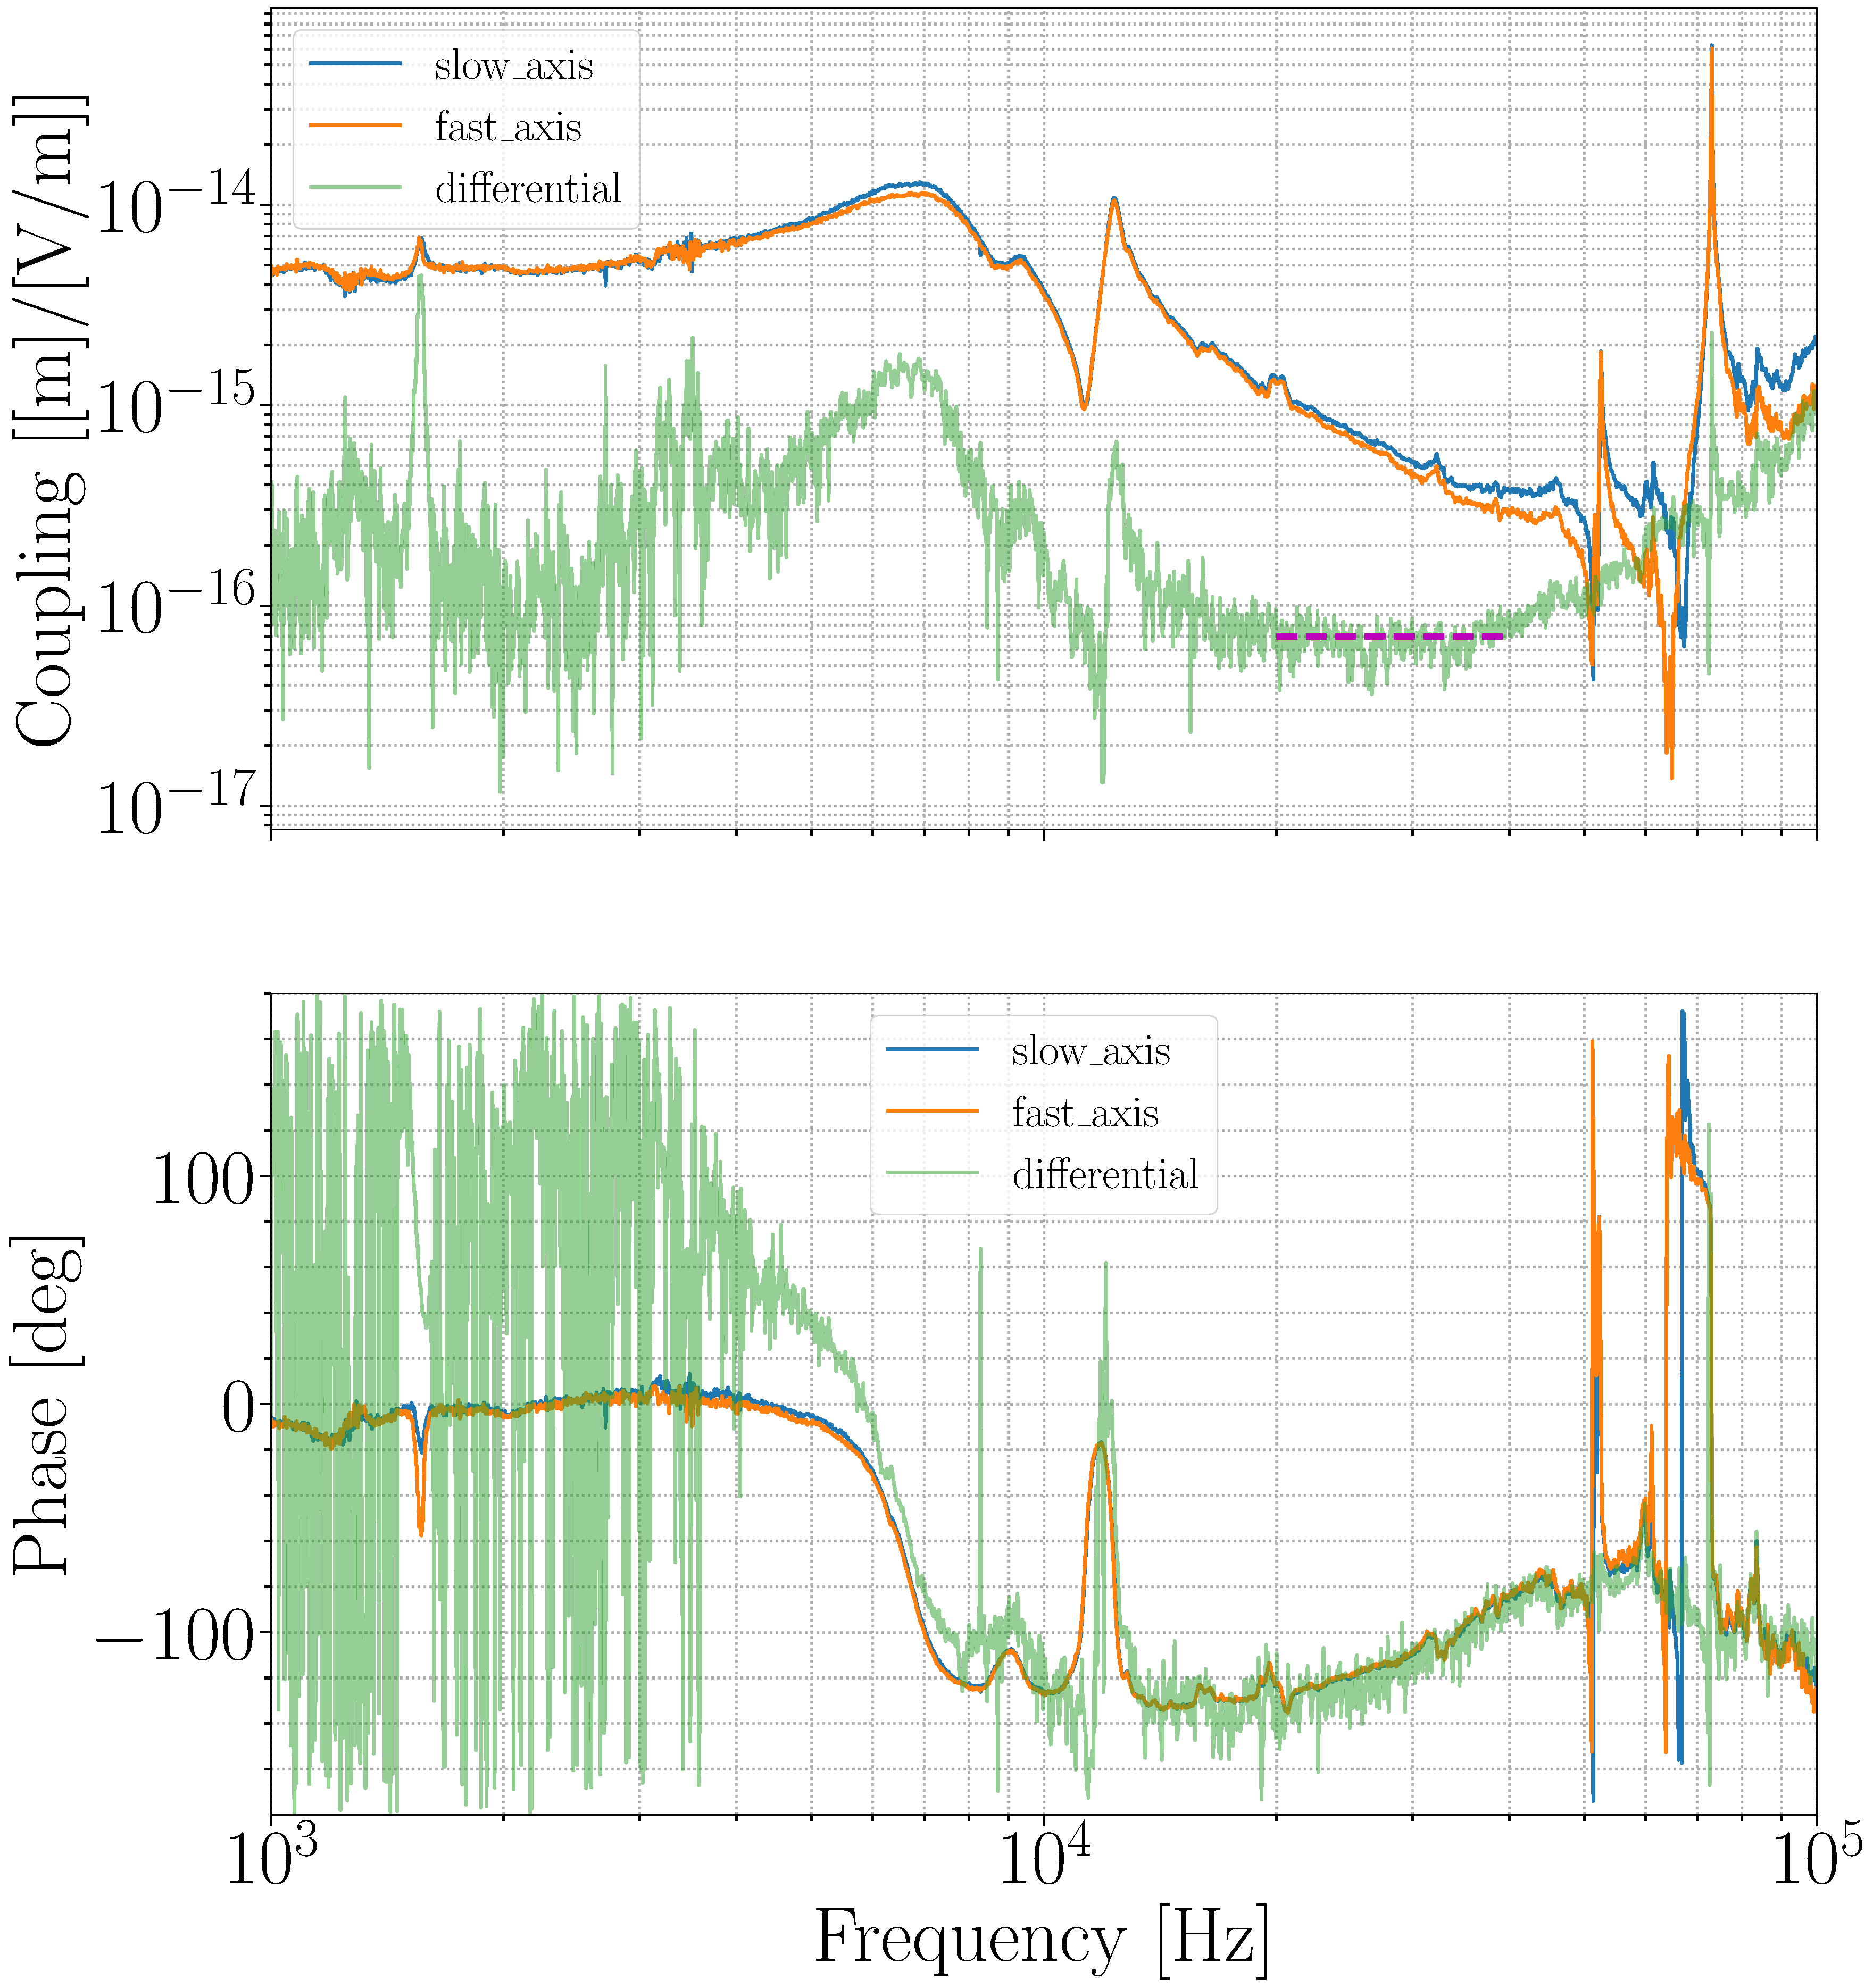
\includegraphics[width=.91\textwidth]{figs/ALGAAS/coupling_tf.pdf}
    \caption{Calibrated measurement of the conversion factor of field strength [V/m] to length [m] when the beam input polarization is aligned along the slow and fast $\gaas$ / $\algaas$ coating axes.}
    \label{fig:final_tf_conversion}
\end{figure}

From this experiment an upper threshold estimate between 20 kHz - 40 kHz is $\approx \; 1.1 \times 10^{-17} \; [\mathrm{m}]/[\mathrm{V}/\mathrm{m}]$ though at higher frequency, frequency dispersion of the electro-optic coefficients may explain the increase.  The uniform flat response is extended to frequencies at which LIGO operates 10 Hz - 1 kHz as prior work has demonstrated such a trend from 10 Hz to several 10s of kHz.

The significantly improved thermal noise performance of $\gaas$/$\algaas$ HR coatings make these crystalline coatings a prime candidate for the core optics in current and future gravitational wave detectors. The measured upper threshold of the electro-optic noise is demonstrated to be $\sim 10^{-26} \; [1/\sqrt{\mathrm{Hz}}]$ two orders of magnitude below the designed noise floor $\sim 10^{-24}\; [1/\sqrt{\mathrm{Hz}}]$ of current and future gravitational wave detectors.

%\begin{itemize}
%\item \textbf{Vibration of plates (Leissa)} \cite{leissa:1969} Computing frequencies and order of magnitude
%	\begin{itemize}
%	    \item Numerical computation (Order of magnitude result)
%	\end{itemize}
%\item \textbf{Steve's COMSOL model results}
%\end{itemize}


